% !TeX spellcheck = en_US
% Paperformat
% tex.stackexchange.com/questions/428553/add-bibliography-as-part-instead-of-chapter-in-toc
\documentclass[a4paper, 12pt, bibliography=totoc]{scrartcl}
\usepackage{setspace}
\renewcommand{\baselinestretch}{1.5} 
%\usepackage{cite}
%\usepackage{ragged2e}

\usepackage{url}
\usepackage{bm} % bold math
\usepackage{nccmath} % medium fraction with mfrac 
\usepackage{caption}
\usepackage{amssymb}
\usepackage{enumitem}
\usepackage{graphicx}
\usepackage{amsthm} % theorems
\usepackage{hyperref}
\usepackage{float}
\usepackage{listings} % code
\usepackage{xcolor}
\usepackage{longtable} % breaks pages
\usepackage{tabularx}
\usepackage{thmtools}
\usepackage{booktabs}
\usepackage[framemethod=TikZ]{mdframed}
\usepackage[export]{adjustbox}

\declaretheoremstyle[
headfont=\bfseries,
notefont=\bfseries,
%notebraces={(}{)},
qed=,
headpunct=.,
headformat={\mbox{\NAME{} \NUMBER}}
%headformat={\mbox{\NAME{} \NUMBER\NOTE}}
]{custom}

\declaretheoremstyle[
headfont=\bfseries, 
notebraces={[}{]},
bodyfont=\normalfont,
headpunct={},
postheadspace=\newline,
spacebelow=\parsep,
spaceabove=\parsep,
mdframed={
	backgroundcolor=blue!10, 
	innertopmargin=6pt,
	roundcorner=10pt, 
	innerbottommargin=6pt, 
	skipabove=\parsep, 
	skipbelow=\parsep } 
]{thmstyle}

\definecolor{eclipseStrings}{RGB}{42,0.0,255}
\definecolor{eclipseKeywords}{RGB}{127,0,85}
\definecolor{deepgreen}{rgb}{0,0.5,0}
\colorlet{numb}{magenta!60!black}
\DeclareFixedFont{\ttm}{T1}{txtt}{m}{n}{12}  % for normal

\lstdefinestyle{custompy}{
	language=Python,
	backgroundcolor=\color{white},
	basicstyle=\normalfont\ttfamily,
	belowcaptionskip=1\baselineskip,
	breaklines=true,
	numbersep=12pt,
	frame=LtRb,
	xleftmargin=\parindent,
	showstringspaces=false,
	keywordstyle=\bfseries\color{orange!80!black},
	commentstyle=\itshape\color{purple!40!black},
	identifierstyle=\color{blue},
	stringstyle=\color{deepgreen},
	emph={self},
}

\lstdefinelanguage{json}{
	basicstyle=\small\ttfamily,
	numbers=left,
	framexleftmargin=5pt,
	backgroundcolor=\color{white},
	commentstyle=\color{eclipseStrings}, % style of comment
	stringstyle=\color{eclipseKeywords}, % style of strings
%	numberstyle=\scriptsize,
	stepnumber=5, firstnumber=1,
	numbersep=15pt,
	showstringspaces=false,
	breaklines=true,
	frame=LtRb,
	string=[s]{"}{"},
	comment=[l]{:\ "},
	morecomment=[l]{:"},
	literate=
	*{0}{{{\color{numb}0}}}{1}
	{1}{{{\color{numb}1}}}{1}
	{2}{{{\color{numb}2}}}{1}
	{3}{{{\color{numb}3}}}{1}
	{4}{{{\color{numb}4}}}{1}
	{5}{{{\color{numb}5}}}{1}
	{6}{{{\color{numb}6}}}{1}
	{7}{{{\color{numb}7}}}{1}
	{8}{{{\color{numb}8}}}{1}
	{9}{{{\color{numb}9}}}{1}
}

\declaretheorem[style=thmstyle, name=Theorem]{thm}
\declaretheorem[style=custom, name=Example]{example}
\declaretheorem[name=Method call]{mycall}

\usepackage[style=alphabetic,backend=biber]{biblatex}
\addbibresource{bibtex.bib}

\definecolor{light-gray}{gray}{0.95}
\lstset{tabsize=2, linewidth=1.05\textwidth, framextopmargin=5pt, basicstyle=\small\ttfamily,numbers=left,backgroundcolor=\color{light-gray}, captionpos=b, breaklines=true, framexleftmargin=5pt, stepnumber=5, firstnumber=1}
\newtheorem{theorem}{Theorem}[section]
\setlength{\textheight}{1.05\textheight}
\newcolumntype{Y}{>{\centering\arraybackslash}X}
\captionsetup{justification=raggedright}

\pagenumbering{roman}
\begin{document}
\def\myauthor{Martin Röbke} 
\def\mycoauthor{Dr. Johannes Fichte} 
\def\mytitle{Visualizing Dynamic Programming on Tree Decompositions} 
\def\mydate{\today} 
\def\myabgabe{31. Juli 2020}
\def\mymatriculation{3949819}
\def\mybirthday{04.03.1995}
\def\myemail{Martin.Roebke@tu-dresden.de}

\begin{titlepage}
%	\vspace*{\stretch{1}}
	\begin{center}
		\textsc{\large 
		{Technische Universität Dresden \\
			Fakultät Informatik} \\
		[8ex]}             
		{\Large\bfseries Bachelor Thesis}           \\[12ex]
		
		{\huge\bfseries \mytitle}                  \\[6.5ex]
		
		\vspace{12ex}
			
		
		{\Large 
			\begin{tabular}{p{0.47\textwidth}l}
			
				\textit{Author:}&  \textit{Supervisor:}\\
				
				\myauthor &  Dr. Johannes Fichte\\
				
			{\normalsize Matrikel-Nr. 3949819}& \textit{Examiner:}\\
				&  Prof. Dr. Stefan Gumhold\\[20ex]
				
			\end{tabular}
		}
		
		\vfill
		\textsc{International Center For Computational Logic 		\\[4ex]}
		\mydate
	\end{center}
	\vspace{\stretch{2}}
\end{titlepage}
\newpage\newpage
%==============================================================================
%============== DECLARATION ===================================================
%==============================================================================
\section*{ }
\thispagestyle{empty}
{\huge\bfseries{Selbstständigkeitserklärung}\vspace{20pt}}

\noindent
 Hiermit erkl\"{a}re ich, dass ich die von mir am heutigen Tag dem Pr\"{u}fungsausschuss der Fakult\"{a}t Informatik~eingereichte Bachelor-Arbeit~zum Thema:
\begin{center}
	\textit{\mytitle}
\end{center}
\noindent
vollkommen selbstst\"{a}ndig verfasst und keine anderen als die angegebenen Quellen und Hilfsmittel benutzt sowie Zitate kenntlich gemacht habe. Ebenso versichere ich, dass diese Arbeit
oder Teile daraus weder von mir selbst noch von anderen als Leistungsnachweis oder als Leistung, die als Prüfungsvoraussetzung
zu erbringen war, andernorts bereits eingereicht wurden. Wörtliche oder sinngemäße Übernahmen aus anderen Schriften
oder Veröffentlichungen in gedruckter oder elektronischer Form sind gekennzeichnet.
Sämtliche Sekundärliteratur und sonstige Quellen sind nachgewiesen und in der Bibliographie aufgeführt.
Das Gleiche gilt für graphische Darstellungen und Bilder sowie für alle Internet-Quellen. \\[20pt]

\noindent
\myauthor, geb. \mybirthday \\\\
\noindent
01309 Dresden, Müller-Berset-Straße 29\\[80pt]


Dresden,  den \myabgabe \hfill .............................
\begin{flushright}
	(Unterschrift)\hspace{1em}
\end{flushright}


\newpage
%==============================================================================
%============== Acknowledgments ======================================================
%==============================================================================
\newpage
\section*{Acknowledgments}
\vspace{5ex}
I would like to thank my advisor Johannes Klaus Fichte for his professional help and introduction to the research topic. Together with Markus Hecher from the TU Wien they provided material, access to hardware and constructive comments during the project.
 I would like to thank my grandfather Walter Hess, who advised me in mathematical questions all my life, and my father, who introduced me to the field of computer science. Last but not least I would like to thank my mother, who also supported me during my studies and all my life. 
 \newpage
%==============================================================================
%============== ABSTRACT ======================================================
%==============================================================================
\newpage
\section*{Kurzfassung}

\vspace{4ex}

Die Beantwortung von Fragestellungen, die sich mit Hilfe von Graphentheorie ausdrücken lassen, ist in vielen Arbeits- und Forschungsgebieten zunehmend interessant und hilfreich.
Probleme wie die boolesche Erfüllbarkeit, oder im Zusammenhang mit Verkehrsströmen, können in Fragestellungen zu Verbindungen und Knoten übersetzt werden.
Wir denken, dass die Verwendung von Graph-Strukturen helfen kann, Algorithmen in diesen und anderen Bereichen weiterzuentwickeln.

In den letzten Jahren hat die dynamische Programmierung auf Baumzerlegungen dazu geführt, dass neue Algorithmen auf Grundlage von Graphstrukturen entwickelt wurden. Dieser Ansatz erwies sich als sehr erfolgreich, wie in \cite{fichtegpusat2} diskutiert wird. Die Problemstellungen werden hier mittels Techniken aus der "parametrisierten Komplexitätstheorie" \cite[S. 2]{dpdbpadl2020} effizient gelöst.
Da die Entwicklung maßgeschneiderter Algorithmen mittels dynamischer Programmierung recht fehleranfällig sein kann, ist eine schnelle und unkomplizierte Visualisierung hilfreich, um weitere Verbesserungen und umfassendere Anwendung der Methodik zu erreichen.\\

Zur Kommunikation der Daten aus den Implementationen
haben wir ein JSON-Schema als API zwischen Löse-Programmen und dem neu geschaffenen Visualisierungswerkzeug \textit{tdvisu}\footnote{tdvisu ist mit GPLv3 Lizenz veröffentlicht: \url{github.com/VaeterchenFrost/tdvisu}} erstellt.

Als zwei Löser und Referenzimplementierungen unserer Visualisierung haben wir \textit{gpusat}\footnote{gpusat ist mit GPLv3 Lizenz veröffentlicht: \url{github.com/Budddy/GPUSAT}} und \textit{dpdb}\footnote{dpdb ist mit GPLv3 Lizenz veröffentlicht: \url{github.com/hmarkus/dpondbs}} ausgewählt. Zwei moderne Programme auf sehr verschiedenen Plattformen - Grafikkarten und relationalen Datenbanken.\\


\newpage
\section*{Abstract}

\vspace{4ex}

Answering questions that can be expressed using graph theory is increasingly interesting in scientific work.
Problems such as Boolean satisfiability, or in connection with traffic flows, can be translated into questions about connections and nodes.
We think that the use of graph structures can help to further develop algorithms in those and other areas.

In recent years, dynamic programming on tree decompositions has resulted in the development of new algorithms than those developed in the decades before. This approach proved to be very successful as discussed in \cite{fichtegpusat2}, tackling the problems with techniques from parameterized complexity \cite[page 2]{dpdbpadl2020}.
Since the development of tailor-made algorithms using dynamic programming can be quite error-prone, a fast and uncomplicated visualization is helpful to achieve further improvements and wider application of the methodology.\\

For further refinement and visualization of the applied dynamic programming,
we specified a JSON template for data transfer between solvers and the newly created visualization tool \textit{tdvisu}\footnote{tdvisu is available under GPLv3 license at \url{github.com/VaeterchenFrost/tdvisu}}.\\

As two solvers and reference implementations of dynamic programming on tree decompositions we chose \textit{gpusat}\footnote{gpusat is available under GPLv3 license at \url{github.com/Budddy/GPUSAT}} and \textit{dpdb}\footnote{dpdb is available under GPLv3 license at \url{github.com/hmarkus/dp\_on\_dbs}} as modern solvers on two very different architectures - GPUs and relational databases.\\


\paragraph{Keywords:}
\textit{Dynamic Programming, Visualization, Graphs, \\
Tree Decomposition, JSON-Schema, Parameterized Algorithmics 
}\leftskip=1.6cm \rightskip=1cm

\leftskip=0pt\rightskip=0pt


%  table
{% \setlength{\textheight}{1.02\textheight}
	\newpage
	
\tableofcontents
}

% chapter on next page
\newpage

%==============================================================================
%============== INTRODUCTION ==================================================
%==============================================================================
\pagenumbering{arabic}
\section{Introduction}
\subsection{Motivation}

The goal of this thesis is to improve the progress in developing dynamic programming solutions on tree decomposition through visualization.

Graph-algorithms and problems regarding graph-related data are increasingly interesting in scientific work, as the applications of interconnected datasets grow. One interesting paper about graphs in (natural) language processing is \cite{jones-etal-2013-modeling}.
Some use cases include fields of interest like cited in \cite{graphUseCases}: % (see also \url{neo4j.com/use-cases})
\begin{itemize}
	\item Network and Database Infrastructure
	\item Recommendation Engines
	\item Artificial Intelligence and Analytics
\end{itemize}

As illustrations of the possibilities for an application, smaller examples from the problem types Boolean satisfiability \textbf{SAT}, model counting SAT \textbf{\#SAT} and \textbf{minimal vertex cover} are presented.
We also show an example of finding  and visualizing a faulty tree-decomposition that occurred during development.


The target audience for this work includes: 
\begin{itemize}
	\item Developers of dynamic programming on tree decompositions for debugging,
	\item Researchers of such algorithms for comparisons and visualizations,
	\item Teachers and students looking for automatic visualization of their problem instances and the solving process.
\end{itemize} 

%The idea for this project comes from my supervisor Dr. Johannes Fichte, who works with many projects such as \href{github.com/hmarkus/dp_on_dbs}{dpdb} on solving monadic second order logic (MSOL) problems using highly parallelized architectures like graphics processing units or state of the art databases.
%One early implementation is published in \cite{evaluationMSO} where for different real world examples the results looked promising
%These projects are very competitive ????REF????? for solving even large instances of those problems.
\vspace{2cm}
{\small{Side remark:}
	Of course, the information we visualize could be extracted as text from the respective solver and then analyzed. But as the saying goes, ``one picture is worth 100 spreadsheets". }
\newpage
%============== Concept ====================================================
\subsection{Research Question}
When developing techniques for dynamic programming for various problems or platforms there can be errors in actual implementations that will be hard to pin down. 

There is some evidence and experience in e.g. \cite{SoftwareVisualization, ELVIZ} that visualization of intermediate and final results can help to understand various issues - such as correctness and efficiency of the algorithms.

As there was no tailored tool for our use case yet, it should be created and integrated into existing tools with a minimum of additional effort.

So our main research questions we want to answer with this thesis are:
\begin{enumerate}
	\item How could a prototype visualization and debugging tool for solvers of MSO logic problems using dynamic programming on tree decompositions look like?
	\item How could an implementation of visualization in existing solvers look like?
\end{enumerate}
\noindent
To answer these questions we have implemented \textit{tdvisu}, a visualization software based on {Graphviz}. 
Our proposed solution is inspired by previous manual visualizations like the two examples in Figure \ref{fig:prevvisus} on page \pageref{fig:prevvisus}.
\begin{figure}[H]
	
	\centering
		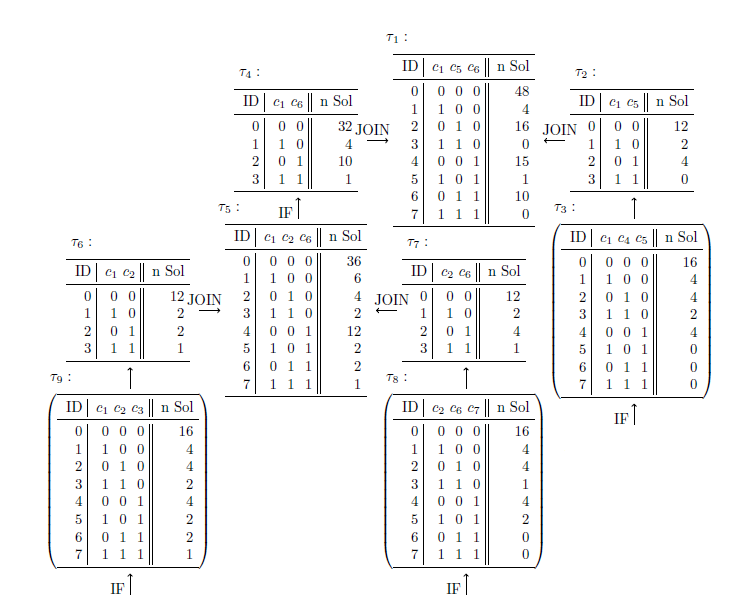
\includegraphics[width=0.9\linewidth,valign=c]{images/DualDA43.png} \\
		
		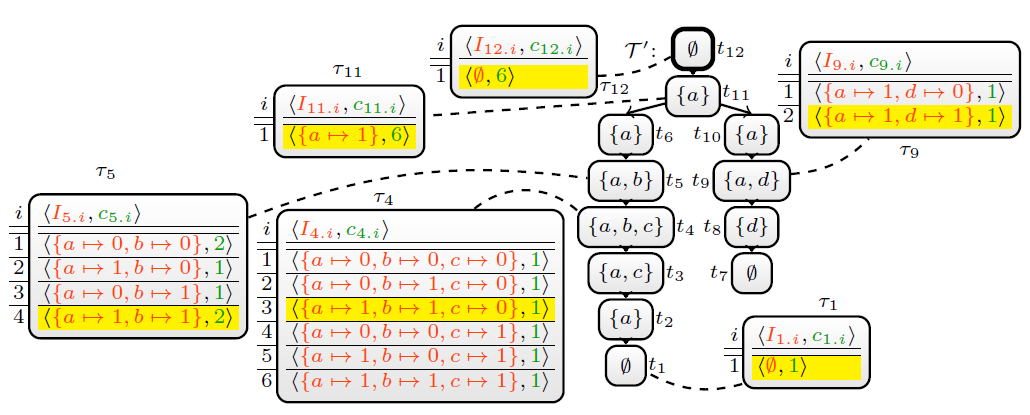
\includegraphics[width=1\linewidth,valign=c]{images/dpdbVisuSat.png}\\ 
	
	\caption[Examples from previous manual visualization]{Two templates from published project documentations which show similar manual visualizations as \textit{tdvisu}. The upper graphic from \cite[Figure 4.3, page 29]{DiplomarbeitZisser} and the lower graphic from \cite[Figure 2, page 4]{dpdbpadl2020}.}
	\label{fig:prevvisus}
\end{figure}

Figure \ref{fig:overviewprog} shows a draft of the process for creating the visualization with \textit{tdvisu}.

\begin{figure}
	\centering
		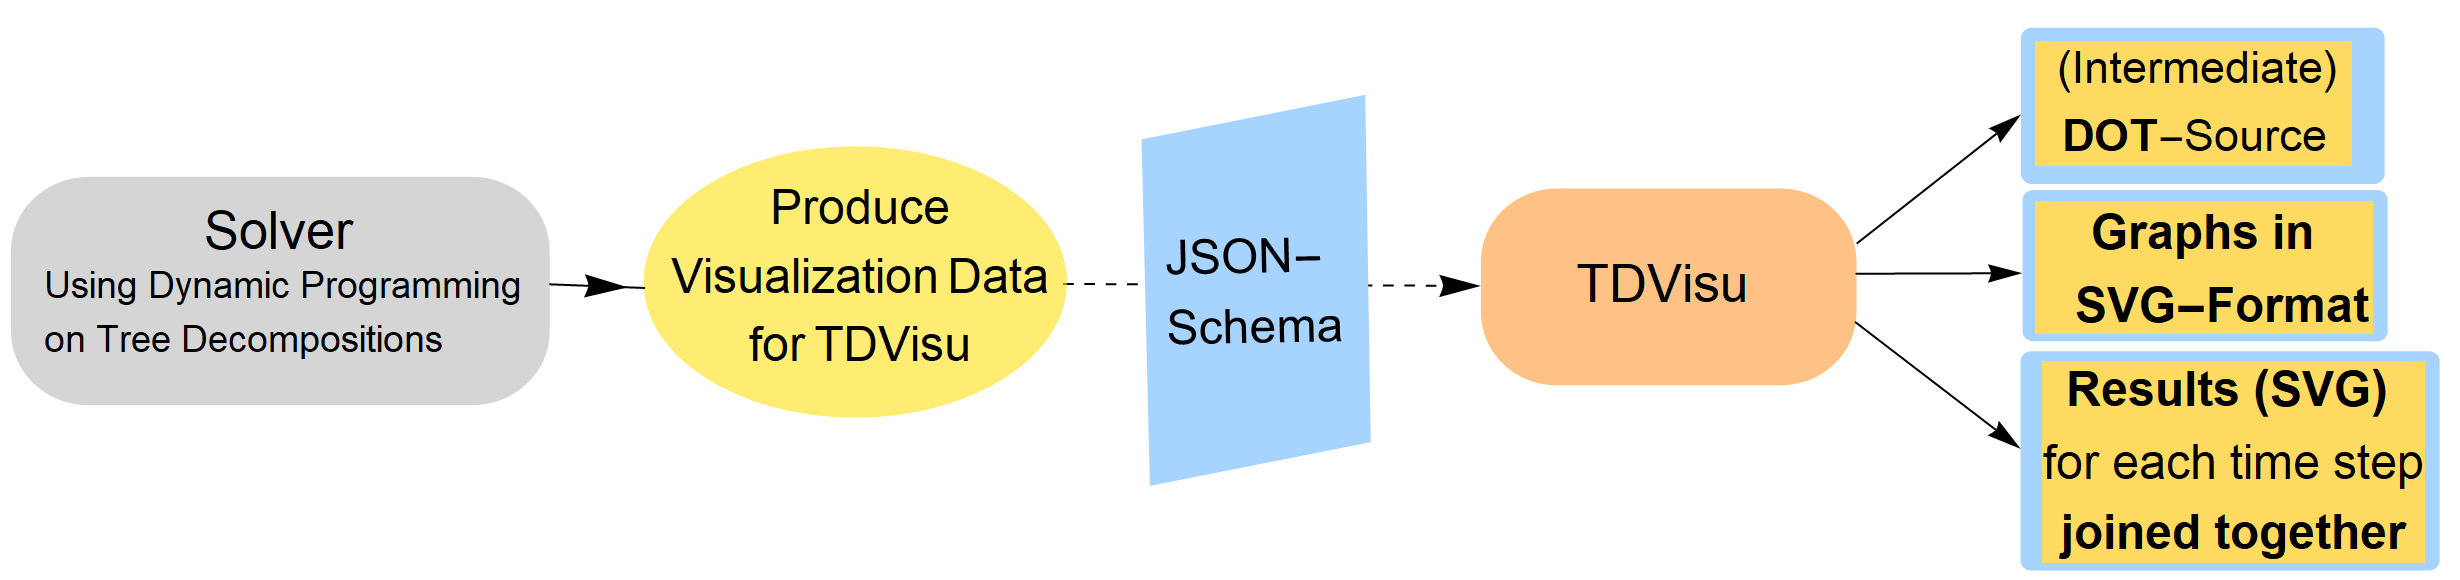
\includegraphics[width=1\linewidth]{images/OverviewProgram.png}
		
	\caption[Visualization Overview]{An overview of the intended use of the visualization. Starting with a solver for DP on TD, over the extraction of the desired data, labels and parameters to the result files.}
	\label{fig:overviewprog}
\end{figure}

\newpage
%============== Outline ====================================================
\subsection{Methodology}

The algorithms we visualize in this thesis use dynamic programming on tree decompositions of graphs.
They preprocess the input graph into a customized tree-decomposition of small tree-width.
This gives the solvers a description of the processing sequence, and allows 
with right hindsight for good parallelization.

The algorithms whose runs we visualize basically work so that the input graph is used to find the best possible processing sequence adapted to the hardware.
With this description it is known which parts of the problem can be solved separately, and which intermediate results have to be stored and for how long. To visualize these algorithms for different problem types, we need to be flexible enough with the data we process for visualization. To accomplish this task, we almost everywhere expect simple text to be included in various places. Only the internal identifiers for nodes or variables in Boolean formulas are not processed based on strings, but on integers.\\

For our visualizations we chose {Graphviz}\footnote{\url{graphviz.org/}} as an open source graph visualization software, which offers customizable visualization for directed and undirected graphs.
The graphs that were used in solving the problem are assembled using the object-oriented style of the Python interface\footnote{\url{pypi.org/project/graphviz/}} to Graphviz.
The tree decompositions in each tested application were provided by the utility {htd} (small but efficient C++ library for computing (customized) tree and hypertree decompositions) \cite{htd}.
The source code for \textit{tdvisu} is available under the GPLv3 license \\on
\mbox{ \url{github.com/VaeterchenFrost/tdvisu}}. Our tool is written in Python and published on PyPI.

We defined a {JSON}-format specification for portability and customization of the visualization in one file and two reference implementations in practical solvers.\\
It is explained in more detail in the implementation chapter, or directly in the \textit{tdvisu/TDVisu.schema.json} file, a JSON-schema\footnote{\url{json-schema.org/draft-07/schema}} with examples and an almost complete validation of the format.

The implementation currently does not support hyper-graphs and assumes that each node in the tree decomposition has either one or two children.
The visualization output consists by default of scalable-vector-graphics (SVG), a very flexible text-based standard for describing images that can be easily compressed (and modified) without loss of quality \cite{SVGMozilla}.


%My previous experiences with the topic of this work mainly come from these two courses:
%\begin{itemize}
%	\item ``Computational Physics" - visualizing with Python and matplotlib, by Prof. Dr. A. Bäcker,
%	chair of computational physics, TU Dresden 2016
%	\item ``Graph Data Management and Analytics" - algorithms and various manipulations on graphs, by Hannes Voigt in 2019. \cite{VLGDMA}
%\end{itemize}

%============== Rel Work ====================================================
\subsection{Related Work}

To the best of our knowledge no comparable tool exists that is capable of out-of-the-box visualization of dynamic programming on tree decompositions.
In this chapter, however, we would like to mention works that deal with the surroundings of our problem.

First two papers dealing with additional solvers exploiting small tree-width and Courcelle's Theorem:
	``Implementing Courcelle's Theorem in a declarative framework for dynamic programming" in \cite{ImplCourcelleDP16};
	and
	``Evaluation of an MSO-Solver" from \cite{evaluationMSO}, indicating that \textit{for some natural optimization problems MSO based approaches might be a suitable alternative to ILP solvers.
	}

%Many computationally hard problems become tractable if the graph structure underlying the problem instance exhibits small treewidth. A recent approach to put this idea into practice is based on a declarative interface to Answer Set Programming that allows us to specify dynamic programming over tree decompositions in this language, delegating the computation to dedicated solvers. In this article, we prove that this method can be applied to any problem whose fixed-parameter tractability follows from Courcelle's Theorem. \cite{ImplCourcelleDP16}
%% Journal of Logic and Computation, Volume 27, Issue 4, June 2017, Pages 1067–1094, doi.org/10.1093/logcom/exv089
%%Published:
%%07 January 2016
%
%A fundamental theorem of Courcelle states that every problem definable in Monadic Second-Order Logic (MSO) is solvable in linear time on graphs of bounded treewidth. In this paper, we report on our ongoing effort to develop a general purpose software tool designed to solve MSO-definable optimization and decision problems on graphs of small treewidth. We discuss the theoretical underpinnings of our tool and present experimental results, which indicate that for some natural optimization problems MSO based approaches might be a suitable alternative to ILP solvers
%\cite{evaluationMSO}. 

%--------- Other Visualization ----------

Additional some references on algorithm visualization and visual debugging can be found in

	 ``ELVIZ: A query-based approach to model visualization" about an approach to visualization, generic regarding both the source model, and the kind and content of the visualization \cite{ELVIZ},
	
	 ``Visualizing Tree Structures in Genetic Programming" about methods to visualize the structure of trees that occur in genetic programming \cite{VisuTDinGP},
	
	 The book ``Software Visualization: Visualizing the Structure, Behaviour, and Evolution of Software" - the first textbook on software visualization, Stephan Diehl, Springer 2007 \cite{SoftwareVisualization}.



Current advancements in dynamic programming on tree-decompositions itself can be found in \cite{dpdbpadl2020} and \cite{taminghightw}. One of the latest papers for \textit{gpusat2} discussed a series of experiments using several benchmark sets for model counting \#SAT and weighted model counting. It compared the then latest versions of publicly available \#SAT solvers, where \textit{gpusat2} could solve the vast majority of the instances and ranked second place \cite[Ch. 5]{fichtegpusat2}. 

The authors of \cite{MetatheoremsforRestrictionsofTreewidth} have investigated \textit{whether the results of Courcelle's Theorem can be improved by focusing on two proper subclasses of the class of bounded treewidth graphs: graphs of bounded vertex cover and graphs of bounded max-leaf number}. They were also able to prove stronger algorithmic meta-theorems for these more restricted classes of graphs. 

Courcelle and Durand recommended in their Article in \cite{FiniteAutomata10} two possibilities of circumventing implementation problems of Courcelle's Theorem. \textit{One possibility is to forget the idea of implementing the general theorem, and to work directly on particular problems $[$...$]$. Another one, explored here $[$...$]$ consists in finding fragments of MSO logic having an interesting expressive power, and for which automata constructions (or other constructions) are tractable.}
%\cite{ELVIZ}
%
%This paper presents methods to visualize the structure of trees that occur in genetic programming. These methods allow for the inspection of structure of entire trees even though several thousands of nodes may be involved. The methods also scale to allow for the inspection of structure for entire populations and for complete trials even though millions of nodes may be involved. Examples are given that demonstrate how this new way of “seeing” can afford a potentially rich way of understanding dynamics that underpin genetic programming. The examples indicate further studies that might be enabled by visualizing structure at these scales. \cite{VisuTDinGP}

%Software visualization encompasses the development and evaluation of methods for graphically representing different aspects of software, including its structure, its execution, and its evolution. Software visualization combines techniques from areas like software engineering, programming languages, data mining, computer graphics, information visualization and human-computer interaction. So far, there exist only anthologies and proceedings about software visualization. With this book, Stephan Diehl has written the first textbook on software visualization. As such it targets both students and teachers in computer science. Topics covered include static program visualization, algorithm animation, visual debugging, as well as the visualization of the evolution of software. The author's presentation emphasizes common principles and provides different examples mostly taken from seminal work. In addition, each chapter is followed by a list of exercises including both pen and paper exercises, as well as programming tasks. 
%Although written mostly for graduate students, the book will also be a source for researchers in both academia and industry, as it will provide a broad and systematic overview of the area including many pointers to tools available today. \cite{SoftwareVisualization}
%
%INCLUDE: NEO4J - Bloom ???????
\newpage
%============== Outline ====================================================
\subsection{Thesis Outline}
The rest of the thesis is structured as follows: \\
Chapters~\ref{sec:bg}~and~\ref{sec:practicalreq} give the reader the necessary background for this thesis. In Chapter \ref{sec:project} we describe our approach to the visualization and the main functionalities of the software. Next, Chapter \ref{sec:gpusat} describes the integration of \textit{tdvisu} into the solver \textit{gpusat}~\cite{DiplomarbeitZisser}. In Chapter \ref{sec:dpdb} we describe the integration with the database-based solver \textit{dpdb}~\cite{dpdbpadl2020}.
Chapter \ref{sec:appl} shows, limited by the page size, small examples for the tested use cases of visualization, starting with a \textit{SAT} example, then a \textit{\#SAT} problem visualized, followed by a \textit{minimal-vertex-cover} example. After these three use cases we show the possibilities of joining single result images together. Finally, the chapter closes with a subsection on how our tool can be used as a support for successful debugging. In Chapter \ref{sec:conclusion} we give a summary of our work and hints for future progress.


%==============================================================================
%============== BACKGROUND ====================================================
%==============================================================================
\newpage
\section{Background}\label{sec:bg}
In this chapter we provide a brief background for this work.

We will start with a short introduction to logic and MSO in \ref{sec:MSO}. Monadic second-order logic (MSO) is a logical language that is suitable for expressing numerous graph properties \cite[p.~41]{Courcelle2012}. In the following summary we would like to introduce MSO as an extension  of first order logic and propositional logic. The concepts and notations from propositional logic are needed for the example applications around Boolean Logic and conjunctive normal forms (CNF); MSO will later be used as the language that describes the use cases of the dynamic programming on tree decompositions.
Then we introduce Courcelle's theorem, which describes important properties of the problems and related bounds for the solvers.
Eventually, tree decompositions are described as a basis for dynamic programming in the next section.
%We begin with a description on SAT and \#SAT as examples for a very general problem that can be described with monadic second order logic (MSOL).
%Furthermore the general case of MSOL will be described, as well as the \textit{DIMACS}-file-format used in the projects.
%The following section describes Tree Decompositions (TDs) which are the basis for our visualization. 
%Finally we shortly discuss Courcelle's Theorem~\cite{Courcelle2012} as a related method of solving these problems.

%====================================================================
\subsection{Graphs}

In this thesis we use the word {graph} for a pair $G=(V_{G},~E_{G})$, where $V_{G}$ is a nonempty set of vertices also called {nodes} and $E_{G}=edg_{G} $ is the binary relation $E_{G} \subseteq V_{G} \times V_{G}$, such that $(x,y)\in E_{G}$ if and only if there exists an edge from $x$ to $y$ if $G$ is directed, and an edge between $x$ and $y$ if $G$ is undirected. For further information on graphs we refer to the common literature, for example \cite[p. {401--412}]{HandbookMathGraph} or more casually in \cite{britannicagraphs}. 

\begin{example}\label{ex:wheelgraph}
	$G$ is an undirected graph with
	\begin{align*}
	 G&=(V_{G},E_{G})\\
	 	 V_{G} &= \{1,2,3,4,5,6,7\}\\
	   E_{G} &= \{(1,2),(1,3), (1,4), (1,5),(1,6), (1,7), (2,3), (3,4), (4,5), (5,6), (6,7), (7,2)\}
	\end{align*}
\end{example}


\subsection{Propositional Logic}
 is a formal system $\mathcal{L} = \mathcal{L}(\mathrm {A},\Omega, \mathrm{Z}, \mathrm{I})$ with
\begin{itemize}
	\item the set $\mathrm {A}$ as a countably infinite set of elements called proposition symbols or propositional variables. These are also called terminal elements.
	\item The set $\Omega$ is a finite set of elements called operator symbols or logical connectives. It is partitioned into disjoint subsets as follows:
	
	$\Omega =\Omega _{0}\cup \Omega _{1}\cup \ldots \cup \Omega _{j}\cup \ldots \cup \Omega _{m}.$.
	
	In this partition, $\Omega _{j}$ is the set of operator symbols of arity j.
	
	$\Omega$ is typically partitioned as follows:
	
	${ \Omega _{0}=\{\bot ,\top \}.}$ 
	
	${\Omega _{1}=\{\lnot \},}$
	
	${ \Omega _{2}\subseteq \{\land ,\lor ,\to ,\leftrightarrow \}.}$

	\item The set $\mathrm {Z}$ is a finite set of transformation rules that are called inference rules when they receive logical applications.
	
	\item The set $\mathrm {I}$ is a countable set of initial points that are called axioms when they receive logical interpretations.
\end{itemize}
%============== SAT ====================================================
\subsection{Boolean Algebra}\label{sec:BSP}
% en.wikipedia.org/wiki/Boolean_satisfiability_problem

%SAT was the first known NP-complete problem, shown by Stephen Cook at the University of Toronto in 1971 \cite{SAT1971}

%\begin{align*}
%\text{literal}&\equiv \text{boolean variable v or its negation} \\
%\text{clause}&\equiv \text{finite set of literals, interpreted as the disjunction} \\
%\text{unit}&\equiv \text{clause with $|$c$|$=1} \\
%\text{CNF formula}&\equiv \text{set of clauses, interpreted as their conjunction} \\
%\text{var}&\equiv \text{set of variables contained in the clause or clause set C} \\
%\text{assignment}&\equiv \text{$\alpha $:var(C) $\to $ \{0,1\}} \\
%\text{satisfiedclause}&\equiv \text{if $\exists $v $\in $ var(c), v$\in $c and $\alpha $(v)=1 or $\neg $v$\in $c and $\alpha $(v)= 0. Otherwise falsified}\\ 
%\text{satisfiedform}&\equiv \text{each clause in the formula is satisfied by assignment} \\
%\end{align*}

In this thesis we use the following symbols for expressions of Boolean algebra:\\

${ \Omega _{0}=\{0 ,1 \}.}$ 

${\Omega _{1}=\{\lnot \},}$

${ \Omega _{2}= \{\land ,\lor \}.}$\\

A propositional logic formula, or Boolean expression, is then built from variables, the logical values $\Omega _{0}$, the operators $\Omega _{1}$ and $\Omega _{2}$ as well as parentheses.

\begin{example}\label{ex:booleanform}
	$B$ is a Boolean expression with\\	
	$B = (\text{v1}\lor \text{v4}\lor \text{v6})\land (\neg \text{v5}\lor \text{v1})\land (\neg \text{v1}\lor \text{v7})\land (\text{v2}\lor \text{v3})\land (\text{v2}\lor \neg \text{v5})
	\land (\neg \text{v6}\lor \text{v2})\land \\
	(\text{v3}\lor \neg \text{v8})\land (\text{v4}\lor \neg \text{v8})\land (\neg \text{v4}\lor \text{v6})\land (\neg \text{v4}\lor \text{v7})$
\end{example}

To describe the usual notation used in solvers for Boolean satisfiability, we also use the following definitions to describe the problem instances denoted in conjunctive normal form (CNF).

A literal is a Boolean variable $v$ or its negation $\neg v$. A $clause$ is a finite set of literals interpreted as their disjunction. A clause $c$ is called $unit$ if $|c|=1$. A CNF $formula$ is a set of clauses and is interpreted as the conjunction of its clauses. We define $var(C)$ as the set of variables contained in the clause or clause set C. As $assignment \alpha$ maps variables in a formula to 0 or 1, $\alpha : var(C)\rightarrow 0,1$. A clause is satisfied by an assignment if for some variable $v \in var(c)$ we have $v \in c \land \alpha (v)=1$ {or} $\neg v \in c \land \alpha(v)=0$. Otherwise the assignment falsifies the clause. An assignment satisfies a formula if each clause in the formula is satisfied by the assignment. \\
%A set C of clauses is 
%\begin{itemize}
%	\renewcommand{\labelitemi}{-}
%	\item \textit{unfalsifiable if there is an assignment that falsifies all clauses in it}. This can only exist when there exists a variable $v \in var(C)$ such that $v \in C$ and $\neg a \in C$. 
%	\item \textit{falsifiable} if there is an assignment that falsifies all clauses in C.
%	\item \textit{satisfiable} if there is an assignment that safisfies all clauses in C.
%	\item \textit{unsatisfiable} if there does not exist an assignment that safisfies all clauses in C.consists in
%\end{itemize}\\
\begin{example}\label{ex:example41}
	For visualization samples we will use the formula from Ex. \ref{ex:booleanform} with the following clause set: $C=\{c_{1}=\{v_{1},v_{4},v_{6}\},
	c_{2}=\{v_{1},\neg v_{5}\},
	c_{3}=\{\neg v_{1},v_{7}\},
	c_{4}=\{v_{2},v_{3}\},
	c_{5}=\{v_{2},v_{5}\},
	c_{6}=\{v_{2},\neg v_{6}\},
	c_{7}=\{v_{3},\neg v_{8}\},
	c_{8}=\{v_{4},\neg v_{8}\},
	c_{9}=\{\neg v_{4},v_{6}\},
	c_{10}=\{\neg v_{4},v_{7}\}\}$
\end{example}
\vskip 12pt
The formula $C$ is for example satisfied by the assignment that maps all variables $var(C)\rightarrow 1$ to $1$. 
All 22 satisfying assignments can be seen in Table~\ref{tab:ex41tabx} on page~\pageref{tab:ex41tabx}.

\paragraph{SAT}The Boolean satisfiability problem {SAT} then consists of the question: 
\begin{mdframed}[leftmargin=3em,rightmargin=3em]
 \textit{Given a propositional formula $\phi$, is there an assignment of the variables in $\phi$ for which $\phi$ is satisfied?} 
\end{mdframed}
\textbf{Example}~\ref{ex:example41} has a satisfying assignment, see Chapter \ref{sec:applsat} for a discussion.\pagebreak

\paragraph{\#SAT}The ``counting problem" of SAT asks the question:
\begin{mdframed}[leftmargin=3em,rightmargin=3em]
\textit{Given a propositional formula $\phi$, for how many assignments of the variables in $\phi$ is $\phi$ satisfied?}
\end{mdframed}
\textbf{Example}~\ref{ex:example41} has 22 satisfying assignments, see Chapter \ref{sec:applssat} for its discussion.\\
\noindent

%SAT Handbook:
%Even finding a single solution can be a challenge
%for such problems; counting the number of solutions is much harder.Not
%surprisingly, the largest formulas we can solve for the model counting problem
%with state - of - the - art model counters are orders of magnitude smaller than the
%formulas we can solve with the best SAT solvers. Generally speaking, current
%exact counting methods can tackle problems with a couple of hundred variables, while approximate counting methods push this to around 1, 000 variables.

% EXAMPLE 4.1?
To later create a tree decomposition for Boolean formulas, solvers use the structure of the clause set to compute at least one of the three following graphs.
For more details see for example \cite[Chapter~2.1]{DiplomarbeitZisser}.

The \textit{primal graph} of a SAT formula contains a vertex for each variable of the SAT formula, and only has an edge between two vertices if they both occur in one clause together.

The \textit{incidence graph} of a SAT formula if bipartite and contains a node for each variable and clause in the SAT formula. It only has edges between a variable node and a clause node if the variable occurs in the clause.

The \textit{dual graph} of a SAT formula contains a node for each clause in the SAT formula. This graph only has an edge between two vertices if the two clauses have at least one common variable.

Those three graphs for our Example \ref{ex:example41} are shown in Fig.~\ref{fig:primalgraph41} .

\begin{figure}[H]
	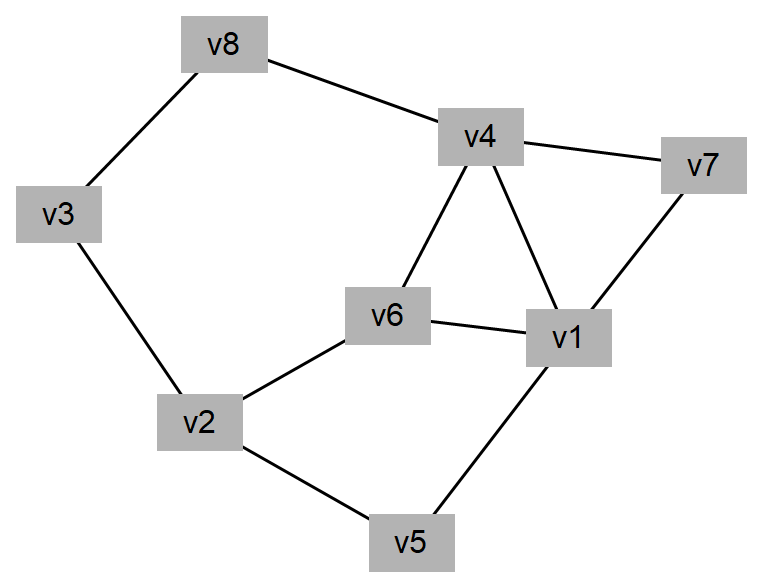
\includegraphics[width=0.33\linewidth]{images/primalgraph41.png}
	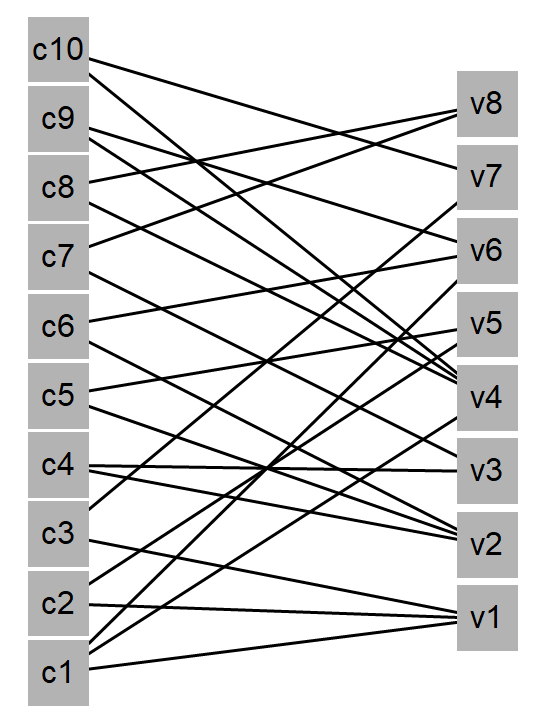
\includegraphics[width=0.32\linewidth]{images/incgraph41.png}
	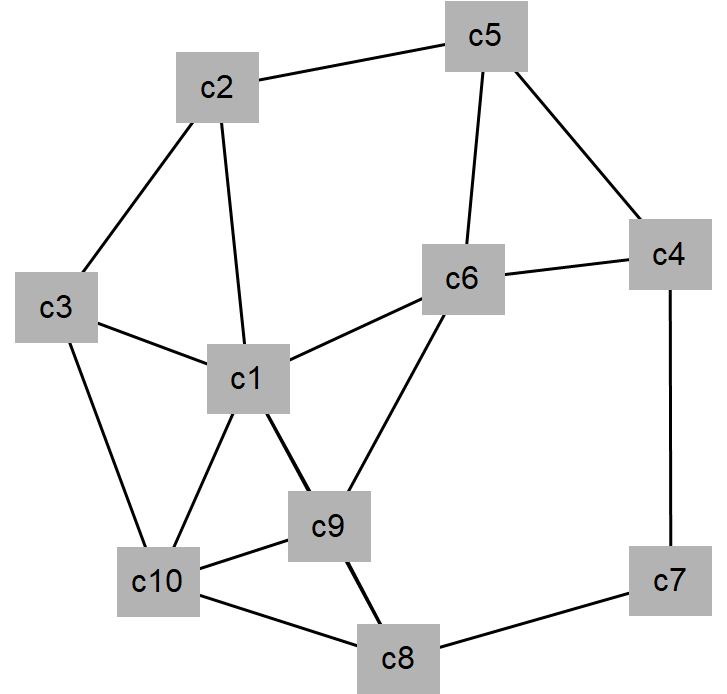
\includegraphics[width=0.33\linewidth]{images/dualgraph41.png}
	\caption[Primal Incidence and Dual Graph]{From left to right: primal, incidence and dual graph of Example~\ref{ex:example41}.}
	\label{fig:primalgraph41}
\end{figure}

\subsection{From Propositional Logic to MSO Logic}

\paragraph{First-order logic} adds relations and quantifiers to propositional logic.
For further information on logic see for example \cite[Chapter~5]{HandbookMathGraph}. \\
The quantifier symbols are
\begin{itemize}
	\item $\exists$ for the existential quantification and
	\item $\forall$ which expresses that a propositional function can be fulfilled by any member of a domain.
\end{itemize}

While \textbf{first-order logic} only quantifies variables that range over individuals (elements of the domain of discourse), \paragraph{Second-order logic}in addition also quantifies over relations.

\paragraph{Monadic second-order logic (MSO)} is a restriction of second-order logic in which only quantification over unary relations (i.e. sets) is allowed. 
%A quantification over functions is therefore also not allowed due to the equivalence to relations.

%Interested in MSO logic over graphs.

%Two types of MSO formulas \textit{or logical graph representations}.
%The expressions have the form: ``There exists a \textbf{set of edges} that is..." can not be transferred into ``set of vertices".
%
%\begin{itemize}
%	\item MSO formulas
%	\item MSO$_{2}$ formulas with edge quantification $\equiv$ MSO formulas over incidence graphs
%\end{itemize}
%\begin{itemize}
%	\item G=(vertices, edges as binary relation)
%	\item INC(G) = (vertices and edges, Inc)
%	for G undirected: Inc(e,v) <-> v is a vertex of edge e
%\end{itemize}
%\begin{itemize}
%	\item FPT for clique width
%	\item FPT for tree-width
%\end{itemize}
%This can also be done for directed graphs!

%============== MSOL ====================================================
\subsection{MSO (Graph) Properties}
MSO logic can express \textbf{graph properties} and \textbf{mappings} from (labeled) graphs to (labeled) graphs \cite{CourcelleGROW}.
Typical MSO properties include:

\begin{itemize}
		\item \textbf{Vertex Cover} \cite[Ch. 4.2]{dpdbpadl2020}\\
	Given a graph $G=(V,E)$ a vertex cover is a set\\
	$C \subseteq V:edg(u,v)\implies \{u,v\}\cap C \neq \emptyset)$\\
	Then minimal vertex cover (MinVC) asks to find the minimum cardinality $|C|$ among all vertex covers of $G$. 
	
	\item \textbf{K-colorability}\\
	Example graph is 3-colorable:\\	
	$\exists X,Y~(X \cap Y = \emptyset \land \forall u,v~(edg(u,v) \implies [(u\in X \implies v\notin X)\land (u\in Y \implies v\notin Y)\land (u\notin X \cup Y \implies c \in X \cup Y)]))$
	
	\item \textbf{Connectivity}\\
	Example graph is \textbf{not} connected:\\	
	$\exists Z~(\exists x \in Z \land \exists y \notin Z \land (\forall u,v~[u\in Z \land edg(u,v) \implies v \in Z]))$

\end{itemize}
More examples of MSO properties can be found for example in \cite[Theorem 3.5]{ARNBORG1991308}.
%\url{youtu.be/Wyn3djrYg7c?t=1385} Bruno Courcelle: Recognizable sets of graphs: algebraic and logical aspects 
%\url{library.cirm-math.fr/Record.htm?idlist=2&record=19276851124910940339}
%Recording during the thematic meeting: ``Frontiers of reconnaissability" the April 29, 2014 at the Centre International de Rencontres Mathématiques (Marseille, France)


%============== TD ====================================================
\subsection{Tree Decomposition}
%Used in RNA Folding: Novel prediction techniques are developed based on graph tree decomposition. \cite{BioInfoTD1970}
%See also chapter 2.2 of \cite{DiplomarbeitZisser}.
%Tree decompositions were originally introduced by Robertson and Seymour \cite{ROBERTSON198449} in 1984.
A \textit{tree decomposition} (TD) of a graph $G$ is a pair $(T, \chi)$. $T$ is a tree and $\chi$ is a mapping which assigns each node $n~\in~V(T)$ 
a set $\chi(n) \subseteq V(G)$ called a \textit{bag}. Then $(T, \chi)$. $T$ is a TD if the following three conditions hold:

\begin{itemize}
	\item[1)] for each vertex $v(n) \in V(G)$ there is a node $n \in V(T)$ such that $v \in \chi(n)$
	\item[2)] for each edge $(x,y) \in E(G)$ there is a node $n\in V(T)$ such that $x,y \in\chi(n)$
	\item[3)] if $x,y,z \in V(T)$ and $y$ lies on the path from x to z then $\chi(x) \cap \chi(z) \subseteq \chi(y)$. The set of bags that contain the variable v induce a connected sub-graph of T.
\end{itemize}
The width $width(T)$ of a tree decomposition $T$ is $max_{n\in V(T)}(|\chi(n)|)-1$.
The tree width of a graph is the \textit{minimal width} over all tree decompositions of the graph. 

%Wiki: In this definition, the size of the largest set is diminished by one in order to make the treewidth of a tree equal to one. 

% Examples
We use tree decompositions throughout our visualizations in this thesis. One detailed explanation is also introduced in \cite{pcgp2019} at page 169.
The tree decomposition for our ``wheel graph" example \ref{fig:wheelgraph} can be viewed in Listing~\ref{lst:wheelgraphtd} on page \pageref{lst:wheelgraphtd}. The conditions for tree decompositions outlined above are easy to verify for this small example, and we get  $width(T)=3$ for this decomposition.
\begin{figure}[h]
	\centering
	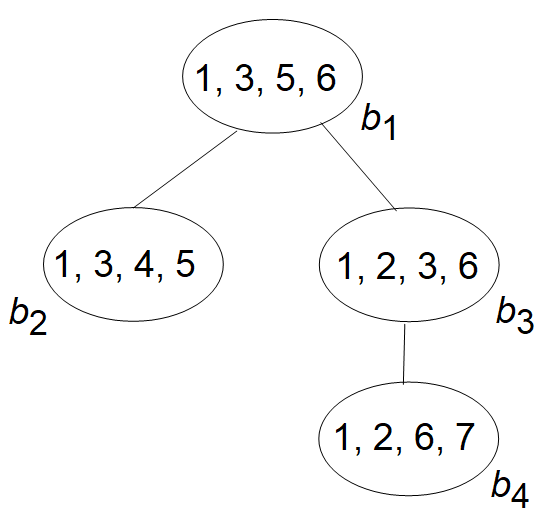
\includegraphics[height=6cm]{images/TDWheelgraph7.png}
		\caption[Tree decomposition of the wheel graph]{Tree decomposition of a wheel graph (Fig. \ref{fig:wheelgraph})	with seven vertices.}
	\label{fig:tdweelgraph7}
\end{figure}

\medskip\noindent
Some projects might use so called \textit{nice} tree decompositions in order to simplify the cases in the used algorithm \cite[Ch.~2.2]{DiplomarbeitZisser}.
For every tree decomposition a nice tree decomposition can be computed within linear time without increasing the width \cite{klokstw}.
Non-nice tree decomposition, however, have advantages in terms of solving time. In the application \textit{gpusat} for example they combined three single operations into one introduce forget (IF) operation. This reduces the overhead for memory operations on the device and the overhead for copying and retrieving tables between devices. Another advantage is that this reduces the size of the tables they need to store by forgetting the variables which do not occur in the next bag after each introduce operation \cite[Ch.~4.2.1]{DiplomarbeitZisser}. 
We see the results of this combined IF operation throughout our visualizations, where for the most part only the results needed for the next bag are included.\\
Similar techniques regarding non-nice TD are also used in the solver dpdb, see \cite[Ch.~4.1]{dpdbpadl2020}.\\

As stated in \cite[Ch.~2.2]{DiplomarbeitZisser}, Arnborg et. al. \cite{arnborgtd} have shown that finding a tree decompositions of minimal width is only feasible for ``small graphs".  There are exact methods for obtaining minimal width tree decompositions,  e.g. \cite{gogatetw, bachoore06}. The solvers for which we implemented the visualization use heuristics  for  generating tree decompositions, therefore  the width of larger examples than shown in this thesis might not be minimal. 


%============== Reference on Algo and Param Complexity ====================================================
\subsection{Dynamic Programming on Tree Decompositions}
In this chapter we want to give a short overview over the basics of dynamic programming. For specific information on the visualized algorithms we refer to \cite{DiplomarbeitZisser, samermodelcounting, dpdbpadl2020}. \\

With dynamic programming, a problem is broken down into parts and the parts are then solved individually. The solving algorithm evaluates the formula along the path of the tree decomposition in a bottom up order starting in one of the leafs. The solution for each assignment in the bag is then stored in a table. The size of the table is exponential to the size of the bag. The tables of the child nodes can be deleted as soon as the table of the current node is generated. \cite[Ch. 3.1]{DiplomarbeitZisser}.\\

The dynamic programming approach for a given graph works as follows:
\begin{enumerate}
	\filbreak
	\item Create a tree decomposition ${T}$ of the graph.
	\item Apply dynamic programming for each bag in bottom up order of ${T}$
	\begin{itemize}
		\item[a)] visit the next node \textit{n} of ${T}$,
		\item[b)] apply the solving algorithm to the bag and
		\item[c)] store the results in a table.
	\end{itemize}
	\item Output the result based on the table of the root node of the tree decomposition.
\end{enumerate}

The basic algorithmic procedure is presented in Fig.~\ref{fig:dpalgo}. It does include a step one to build a graph in case the type of problem (like SAT) requires it.
\begin{figure}[h]
	\centering
	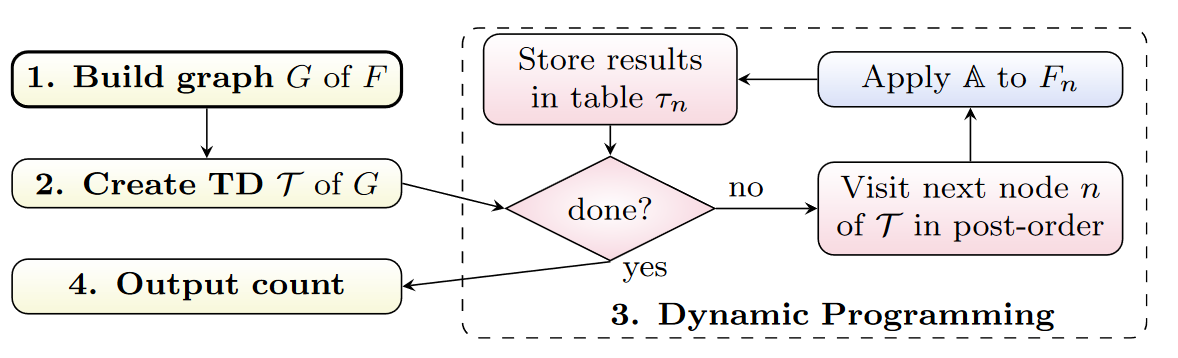
\includegraphics{images/DPAlgo31.png}
	\caption[Basic procedure for dynamic programming on TD]{ Basic procedure for dynamic programming on TD. Source: \cite[Figure~3.1]{DiplomarbeitZisser} }
	\label{fig:dpalgo}
\end{figure}

\pagebreak
\subsection{Parametrized Complexity}
In the following two section we want to introduce the reader with some computational bounds for the underlying concept and problems of solving MSO-problems with the current approaches.

%\subsubsection{Fixed-Parameter Tractable (FTP-)Algorithm}

% en.wikipedia.org/wiki/Parameterized_complexity
\paragraph{FPT for model checking}
Some problems can be solved by algorithms that are exponential only in the size of a fixed parameter while polynomial in the size of the input. Such an algorithm is called a fixed-parameter tractable (FTP-)algorithm, and the problem can be solved efficiently for small values of the fixed parameter \cite{ParamCompGrohe}.
%\begin{thm}
%	An algorithm is FPT if it takes time $f(k)\cdot n^{c}$ for some constant $c$ and a fixed function f depending only on $k \in \mathbb{N}$. The size of the input is n. 
%	The value k is a parameter of the input, in our case usually tree-width. 
%	This algorithm is then usable for small values of k.
%\end{thm}

% Implications
There are efficient algorithms for enumerating and for counting the number of solutions of a MSO formula, if it is ensured that the input data is preprocessed in linear time, and that each solution is then produced in a delay linear in the size of each solution \cite{MSOQueriesGuillaume, ARNBORG1991308}.
MSO graph properties are ``fixed-parameter-tractable" with respect to tree-width. So are MSO counting and optimizing functions \cite{CourcelleGROW}.

%DETAILS MinVC: 
%en.wikipedia.org/wiki/Vertex_cover#Fixed-parameter_tractability

%============== Courcelle ====================================================
\paragraph{Courcelle's Theorem}
 Courcelle's theorem is a constructive meta-theorem that provides algorithms for evaluating MSO formulas over graphs of bounded treewidth.
Courcelle's theorem:

\smallskip\noindent
\textit{
	Every graph property definable in monadic second-order logic (MSO) is decidable in linear time on graphs of bounded tree-width. }\leftskip=1.5cm\rightskip=2cm

\leftskip=0cm\rightskip=0cm\smallskip

\noindent
To be more specific: It holds that for all $k \in \mathbb{N}$ and MSO-formulas F is the decision problem for a given graph G, whether $G \models F$ is true, in time $2^{p(tw(G))} \cdot |G|$ with a polynomial p decidable \cite[p. 54--56]{Courcelle2012}.\smallskip 

\noindent
%A generic workflow implementing Courcelle's theorem looks like we see in Figure~\ref{fig:UsageCourcelle}.
%\begin{figure}[H]
%	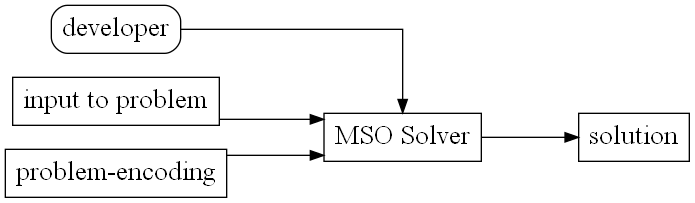
\includegraphics[height=0.2\textheight]{images/UsageCourcelle.gv.png}
%	\caption{Implementation sketch of Courcelle's Theorem}
%	\label{fig:UsageCourcelle}
%\end{figure}

The challenge now is that naive implementations, even if they are linear in the size of the input, are still expensive and the constant factor can be very significant \cite{Courcelle2012,KNEIS200965,MetatheoremsforRestrictionsofTreewidth}. 
A recommendation in~\cite{FiniteAutomata10} is to \textit{forget the idea of implementing the general theorem, and to work directly on particular problems}. An efficient implementation will require several tricks to make this approach practical~\cite{DiplomarbeitZisser,fichtegpusat2}. Developing and debugging these ``tricks" is not always that easy, so a visualization can help at this point.\smallskip 


%==============================================================================
%============== Practical Requirements ========================================
%==============================================================================

\section{Practical Requirements}\label{sec:practicalreq}
The exchange of intermediate results from solvers and parts of the visualization utilizes two defined file formats. In the following two chapters we want to introduce the reader with the concepts of the DIMACS and DOT format. These formats are either produced or required as input at various stages of the application.
  
%============== DIMACS ====================================================
\subsection{DIMACS format}

Inputs for solvers and in some cases for preparing the visualization of dpdb are usually in a DIMACS format. There exist several standardized formats for different cases, for example CNF clauses, graph edges and graph decompositions.
Several file formats for these purposes were developed at ``DIMACS" (the Center for Discrete Mathematics and Theoretical Computer Science) \cite{dimacsimplcha} beginning in 1993 at Rutgers University.
They are also partly supported in several math-related software like \textit{MATLAB}~\cite{matlabcnf}, \textit{Maple}\footnote{\url{www.maplesoft.com/support/help/maple/view.aspx?path=Formats/CNF}} or \textit{Mathematica}\footnote{\url{reference.wolfram.com/language/ref/format/DIMACS.html}}.

The underlying concept is a line-based ASCII file. For all different formats we read comments as lines starting with the character ``c", a problem line starting with ``p" (rarely with ``s"). Following then the problem line and usually multiple lines specifying the data in a format depending on the problem type.
The formats used for this work are:

\paragraph{DIMACS CNF}: This format is used to define a Boolean expression, written in conjunctive normal form. The problem line specifies the type, \textbf{number of variables} and \textbf{number of clauses}. The following lines specify the clauses a positive literal is denoted by the corresponding number, and a negative literal is denoted by the corresponding negative number. Each clause is followed by the character zero, so 0 should not occur as a variable. Instead variables are expected to start at one.

\paragraph{DIMACS tw}: This format is used to describe a single undirected graph. The problem line specifies the type, \textbf{number of nodes} and \textbf{number of edges}. The following lines specify the edges with two nodes separated by a space.

\paragraph{DIMACS td}: This format is used to describe a tree decomposition. The problem line specifies the type, \textbf{number of bags}, \textbf{maximum size of the bags} and \textbf{number of nodes}. The following lines describe the bags starting for each with ``b", the \textbf{bag number} and \textbf{nodes in this bag}. Following these bags are lines not prefixed with a ``b". Now each line describes one \textbf{edge between the bags} as two bag numbers separated by a space.

%Supported also in Maple \url{www.maplesoft.com/support/help/maple/view.aspx?path=Formats/CNF}
\noindent
Examples of this format can be seen in the appendix on page~\pageref{app:input}.

%============== DOT ====================================================
\subsection{DOT format}
The graph description language DOT can be used to describe directed or undirected graphs and specify layout details and various attributes for graphs, edges and nodes. It is similar to the Graph Modeling Language\footnote{gephi.org/users/supported-graph-formats/gml-format} that is used in Chapter \ref{sec:chagraphoutput} as a text based file format for describing graphs. Keeping this in mind, in this chapter we restrict ourselves to a short introduction of the DOT properties that were used the most.

%=========================== DOT Language ====================================

%Dot Language: www.graphviz.org/doc/info/lang.html

The complete abstract grammar for DOT can be viewed at the website of the DOT language \url{graphviz.gitlab.io/_pages/doc/info/lang.html}.\\


The nodes in the DOT-language are \emph{labeled}, so creating a node takes one string identifier and might additionally be provided with a text label. Valid examples for IDs include all combinations of letters and digits.

The optional text labels an have various formats. One example with the setting ``shape=box''

%It supports directed (\textit{digraph} with edges indicated by '->') an undirected (\textit{graph} with edges indicated by '-{}-') graphs.
The visualizations presented in the thesis are constructed as undirected graphs, but would be easily extendable to directed representations, since the order of the edge endpoints remains intact in almost all operations.

Another concept utilized were the sub-graphs and clusters available in DOT.
To get a well structured (bipartite) incidence graph, each partition is placed in an individual cluster, making adjustments to various distances simple.\\


%Attributes (new site): www.graphviz.org/doc/info/attrs.html
DOT has different components which can be modified with attributes: edges, nodes, the root graph, subgraphs and cluster subgraphs, respectively.\\
We want to introduce the reader with the attributes that are modifiable in several places of the visualization - for a more comprehensive breakdown of all possible attributes see \url{www.graphviz.org/doc/info/attrs.html}.

\begin{itemize}
	\item \textbf{rankdir -} one of (``TB", ``LR", ``BT", ``RL"), corresponding to directed graphs drawn from top to bottom, from left to right, from bottom to top, and from right to left, respectively.
	
	\item \textbf{fillcolor -} The color used as a node-background in different situations, for different values see footer\footnote{\url{graphviz.org/doc/info/attrs.html\#k:color}}.  
	In our default values this is always a linear fill; If the value is a ``colorList", a gradient fill is used. 
	
	\item \textbf{fontcolor -} Color for text in nodes or graphs. 
	
	\item \textbf{style -} Drawing style of the nodes.
	At present, the recognized style names are ``dashed", ``dotted", ``solid", ``invis" and ``bold" \textbf{for nodes and edges},  and ``filled", ``striped", ``wedged", ``diagonals" and ``rounded" \textbf{for nodes} only.
	
	\item 
	\textbf{margin -} Used for horizontal and vertical margins around graphs.
	
	\item \textbf{fontsize -} Font size, in points. 
	
	\item \textbf{penwidth -} Specifies the width of the pen in points. This is used to draw lines and curves, including the boundaries of edges and clusters. 
	
	\item \textbf{nodesep -} In dot, this specifies the minimum space between two adjacent nodes in the same rank in inches. 
	
	\item \textbf{shape -} Controls how nodes are drawn. For a full list of shapes see footer\footnote{\url{graphviz.org/doc/info/shapes.html}}. 
\end{itemize} 
\pagebreak
There are three main ways of specifying shapes, and all are applied in our visualization: 
\begin{enumerate}[label=(\arabic*)]
	\item \textbf{polygon-based}; for example as a box, ellipse or diamond.\vspace{10pt}\\		
	\textbf{Example}: shape~=~\textit{diamond};\quad label~=~v\_1
	
	\item \textbf{record-based} nodes that are basically boxes stacked vertically and horizontally and each filled with text.\vspace{10pt}\\
	\textbf{Example}: shape~=~\textit{record};\quad label~=~$\{\text{sol bag 2}|\{\{v1|1|1|1|1|0\}|\{v3|1|0|0|1|1\}$ \\
	\hspace*{0pt}\hfill $|\{v5|0|1|0|1|1\}|
	\{\text{size}|3|3|2|3|3\}\}|\text{min-size: 2}\}$
	
	\item \textbf{HTML-like} labels are specified in a own grammar and can contain tables, text-styles like italic, sub- and superscript, vertical and horizontal rules.\vspace{10pt}\\		
	\textbf{Example}: shape~=~\textit{box};\quad label~=
	\begin{lstlisting}[xleftmargin=0.5cm, xrightmargin=1.5cm, framexleftmargin=5pt]
		<<TABLE BORDER="0" CELLBORDER="0" CELLSPACING="0">
		<TR><TD BGCOLOR="white">bag 1</TD></TR><TR>
		<TD PORT="anchor"></TD></TR><TR><TD>[1, 3, 5, 6]</TD> </TR><TR><TD>dtime=0.0009s</TD></TR></TABLE>>
	\end{lstlisting}
	
\end{enumerate}



%==============================================================================
%============== PROJECT =======================================================
%==============================================================================
\newpage
\section{Implementation}\label{sec:project}

In this section we want to give a thorough insight into the functionalities of \textit{tdvisu}.\\

\noindent As a brief overview our software \textit{tdvisu} works as follows:

\begin{enumerate}
	\item We generate data using a special solver extension or extra programs and extract arguments for the visualization into one file following our JSON schema\footnote{\url{github.com/VaeterchenFrost/tdvisu/blob/master/TDVisu.schema.json}}.
	\item We read the data and parameters into the visualization.
	\item The program creates a graph-layout for the bags of the tree decomposition and calculates which parts are to be shown at each step of the provided solving process.
	\item It creates a graph-layout for each additional graph to visualize alongside the steps in the tree decomposition.
	\item Each graph for individual time steps is saved as a SVG file.
	\item If desired, the individual parts of a time step can be merged into a single SVG file.
\end{enumerate}

As a programming language we chose Python because of its rich dependency environment, fast prototyping, simple tooling for debugging with pdb, optional static analysis with mypy, easy to follow code-style using pylint and autopep8, and modern packaging with pip and PyPI.
Python 3.8 was the latest Python release at the beginning of the project and was used to support ``f-strings". 
%The innovation most frequently applied in this project was the f-string support for shorter and easier to read string-building. %\href{docs.python.org/3/whatsnew/3.8.html}{summary of release highlights}.

The development process for most parts of the final software was driven by evolutionary prototyping using small and well understood examples such as Example~\ref{ex:example41}. It helped to understand the possibilities of visualization in this domain and gather user input and requirements early \cite{rapidPrototypingOvermyer}. Some artifacts of the early prototypes with different graph-description languages can still be seen in the class \textit{Graphoutput} in Section~\ref{sec:chagraphoutput}.

%============== CMD Config ====================================================
\subsection{Commandline and Configuration}

The \textit{tdvisu.visualization} main method expects the command line parameters in a format described by Table~\ref{tab:optionstdvisu}.\\*
\begin{longtable}{|r|p{10cm}|}
	\hline
	Option & Description\\
	\hline\hline
	\endhead

	infile=stdin &  \looseness=-1 Input for the visualization must conform with the TDVisu.schema.json\\
	outfolder &  Folder name to output the visualization results to\\
	-{}-loglevel  & set the minimal loglevel for the root logger\\
	-{}-version & show program's version number and exit\\
	-h, -{}-help & show the help message and exit\\
	\hline\hline
	\caption{Usage of \textit{visualization.py}
		\label{tab:optionstdvisu}}
\end{longtable}\nopagebreak

We see that this command line input is very simple, while the heavy lifting is done with the input given in \textit{infile}.

One extra possibility for configuration is the fine tuning of the logger.
The \textbf{loggers} we use in our project 
%are located in 
%\begin{itemize}
%	\item root, level: WARNING
%	\item visualization.py, NOTSET
%	\item svgjoin.py, NOTSET
%    \item reader.py, NOTSET
%	\item construct\_dpdb\_visu.py, NOTSET
%	\item utilities.py, NOTSET
%\end{itemize} and
can be individually customized using a configuration file.
%comes with the method \textbf{logging\_cfg} from {tdvisu.utilities}. 
There are two example configurations provided with our project, one in the .yml, one in the .ini format. 
%The implementation is very flexible in detecting which parser has to be applied - either via a dictionary-like or a configuration-like function. Both possibilities are documented in Python's {logging configuration}\footnote{\url{docs.python.org/3/library/logging.config.html\#logging-config-api}}.

%Our default configuration in \textit{tdvisu/logging.yml} and \textit{tdvisu/logging.ini} provides one handler, two formatters and six loggers.
%
%The \textbf{handler} is a stream handler to sys.stdout with level \textit{WARNING} and the the 'full'-formatter to format messages.

%The \textbf{full-formatter} includes the full date and time up to milliseconds. After that we can expect the logging-level, filename and line where it was generated, and the message itself.


%With the command line parameter \textit{-{}-loglevel} we can modify the level of \textit{root} and its associated handlers.

%============== Init ====================================================
\subsection{Initialization and Tree Decomposition}

The main purpose of the initialization is parsing the input file containing visualization information.

To get a small overview of the type and structure of the data processed in the software, let us take a quick look at the initialization with the API. We instantiate a \textit{Visualization} object as shown in Listing~\ref{lst:visuinitsmall} , which parses the \textit{VisualizationData} with the help from our \textit{inspect\_json} method. \pagebreak

\begin{lstlisting}[style=custompy, caption={Overview of data initialization}, label={lst:visuinitsmall}]
def __init__(self, infile, outfolder) -> None:
self.data: VisualizationData = self.inspect_json(infile)
self.outfolder = outfolder
self.tree_dec_digraph = None

def inspect_json(self, infile) -> VisualizationData:
visudata = read_json(infile)

# [...] some details skipped
_incid = visudata['incidenceGraph']
_general_graph = visudata['generalGraph']
_svg_join = visudata.get('svg_join', None)

# [...] some details skipped		
return VisualizationData(incidence_graph=incid_data,
general_graph=general_graph_data,
svg_join=svg_join_data, 
**visudata)
\end{lstlisting}

%This is encapsulated in \textit{read\_json}.

Next, we want to extract information into the following places: 
\begin{itemize}
	\item the instance variables 
	\begin{itemize}
		\item \textit{timeline}, describing the time steps on the tree decomposition
		\item \textit{tree\_dec}, describing the TD itself
		\item \textit{bagpre}, \textit{joinpre}, \textit{solpre} and \textit{soljoinpre} as names for different nodes in the produced visualization
	\end{itemize}
	\item The \textit{VisualizationData} object containing the data for 
	\begin{itemize}
		\item IncidenceGraphData in Listing~\ref{lst:incidencedata} page~\pageref{lst:incidencedata}
		\item GeneralGraphData in Listing~\ref{lst:gengraphdata} p.~\pageref{lst:gengraphdata}
		\item SvgJoinData in Listing~\ref{lst:svgjoindataclass} p.~\pageref{lst:svgjoindataclass}
		\item further parameters, which influence additional aspects of the visualization
	\end{itemize}
\end{itemize}

Our next step is to begin visualizing the time steps on the tree decomposition. Specific results of this task can be seen in Chapter~\ref{sec:applsat}, Fig. \ref{fig:DA4SAT_TDStep1}, Tab. \ref{tab:DA4SAT_TDStep2345} and Figure \ref{fig:DA4SAT_TDStep6}.\\

First, a quick setup is performed for the tree decomposition as a directed graph that 
\begin{itemize}
	\item is \textit{strict}, meaning a simple graph where equal edges are merged into one
	\item has an orientation where it grows with each ``rank" of the nodes
	\item has a shape and a fill-color for its nodes.
\end{itemize}

Second, it creates the basic bag structure by adding nodes and edges for all bags of the provided tree decomposition.

Next comes the iteration over the requested time steps, adding the provided solutions and the edges connecting them to the existing bags. We do this in two passes.  A first one in which we move all nodes to their final position. Here a special case occurs when two bags are joined together.
In this case we remove all previous edges between the children and the parent node, add the result to the graph, and add edges from the children to the result and from the result to the parent node. Details of this step can be seen in Listing~\ref{lst:forward-iterate} on page~\pageref{lst:forward-iterate}. \\
And a second pass in which we create the actual images of time steps backwards by masking solutions that were calculated later. The goal is to have all parts of the graphic in optimal position at first appearance and that they do not need to be moved when additional features are added. For details of these steps, see the Listing \ref{lst:backward-iterate} on page~\pageref{lst:backward-iterate}.\\

An automatically inserted join node is shown in Figure~\ref{fig:g41Digraph} on page~\pageref{fig:g41Digraph}.
The provided data for this example to layout the bags can be seen in Listing\ref{lst:edgearray41}. There we see that bags 2 and 3 have an edge to bag 1 and therefore a join-operation will occur between the results of bags 2 and 3:

\begin{lstlisting}[language=json,caption={Structure provided for bags of example \ref{fig:g41Digraph} },xleftmargin=5.5cm,xrightmargin=5.8cm,label={lst:edgearray41}]
"edgearray" : [
	[ 1, 0 ],
	[ 2, 1 ],
	[ 3, 1 ],
	[ 4, 3 ]
]
\end{lstlisting}
\noindent
For rendering the tree decomposition we have added a convenience option to \textit{view} the result files automatically, which is disabled by default.

%============== Timesteps ====================================================
\subsection{Visualizing Additional Graphs}
To gain a more comprehensive insight into the solution process, we want to see the graphs that best describe the problem instance that the solver has been working on.

Because the data in the API does not directly include details about highlights corresponding to time steps in additional graphs, we will construct this information on the fly by referencing with the tree decomposition.


With additional data from the \textit{IncidenceGraphData} class we are further able to reconstruct the
\begin{itemize}
	\item incidence graph,
	\item primal graph,
	\item dual graph
\end{itemize}
for Boolean formulas.

For general problems and with the data from the \textit{GeneralGraphData} class we can construct a simple graph that logically should include the nodes which are in the bags of the TD.\\
% ----- Example for isolated nodes -------
Because graph representations of Boolean formulas are not necessarily connected, we make sure to include potentially isolated nodes into our graphs as well and not only draw some components of it.
For example the formula 
\begin{gather*}
(\neg a\lor \neg b\lor \neg c\lor \neg d)\land (b\lor c\lor d)\land g
\end{gather*}

with its set of clauses 
\begin{gather*}\{c_{1}=\{-a,-b,-c,-d\},c_{2}=\{b,c,d\},c_{3}=\{g\}\}\end{gather*}
will create the dual graph in Fig. \ref{fig:disconnected123}. This happens with no pre-processing and if the variable g is only included in the unit $c_{3}$.

\begin{figure}[H]
	\centering
	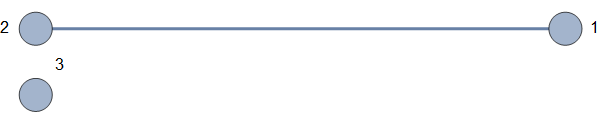
\includegraphics[width=0.3\linewidth]{images/disconnected123.png}
	\caption{Disconnected (dual) graph}
	\label{fig:disconnected123}
\end{figure}

%============== Incid ====================================================
\subsection{Incidence Graph}\label{sec:incid}

The idea is to visualize the incidence graph as a bipartite graph for clauses and variables that can represent the formula the solver did work on in those problem instances.

\begin{figure}[H]
	\centering
	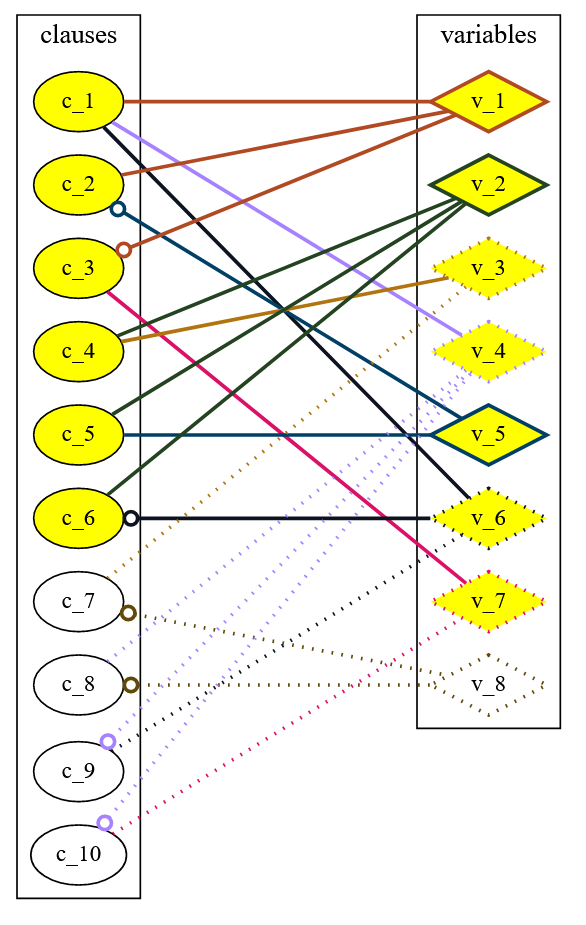
\includegraphics[width=0.4\linewidth]{images/IncidenceStep6.png}
	\caption[Example for the incidence graph]{Example for the incidence graph constructed from Ex. \ref{ex:example41}.}
	\label{fig:incidencestep6}
\end{figure}

 We can see the incidence graph visualization for our example Boolean formula in Figure~\ref{fig:incidencestep6}. On the left side we see the clauses ordered by their label, each in an ellipse-shaped node. The other partition does contain the sorted variables in diamond-shaped nodes. As an addition to its visualization we did include the negations as the little circles on the left end of each edge where a negated variable is included in the respective clause. The right-hand partition does get the different \textit{colors} applied to its nodes and their adjacent edges.
 
 We emphasize the clauses their nodes used in each timestep with a changing background and the not used dotted edges. This allows the correlation of the  parts of the formula with the bags.  

The representation of the bipartite graphs can be adjusted in many parameters; including colors, fontsize, fillcolor and more, Listing \ref{lst:incidencedata} on page~\pageref{lst:incidencedata}.

%We create the graph, add the necessary arguments and two sub-graphs. 
%The first subgraph is called \textit{cluster\_clause} with its label \textit{clauses}.
%We add the clauses with their clause-ids starting at one sorted in ascending order from top to bottom.

%The second sub-graph we call \textit{cluster\_ivar} labeled \textit{variables} gets all variables added to it, 
%starting from variable-id one. 
%This sub-graph does get the different provided \textit{colors} applied to its nodes and their adjacent edges.

%The last step in this method is the highlighting of ``active" parts in each time step beeing processed during its dynamic programming. To accomplish this with as small overhead as possible, we apply and remove additional lines to the body of its graph source code. 
%For highlighting there are two main cases:
%\begin{itemize}
%	\item There is no active clause in this step: we only reset highlighting
%	\item Else: we also create new highlighting for clauses, variables and edges
%\end{itemize}
%In each case we create one image after the step to provide the inside generated.

%============== General Graph ====================================================
\subsection{General Graph}
This type of graph can represent the underlying graph for different problems, as well as primal and dual graph for Boolean formulas.
Because of its wider scope, the layout for the general graph was not as simple to create as for the incidence graph.
We did prepare two different layouts that should cover most cases and are toggled by the parameter \textit{do\_sort\_nodes}.
For smaller and dense graphs of up to 20 vertices it might be helpful to sort the nodes on a circle, while for larger or sparse graphs an organic layout may be more appropriate.

To layout these two variants, we selected the engine depending on
\begin{itemize}
	\item \textit{do\_sort\_nodes} true: circo (see \cite{ST99})
	\item \textit{do\_sort\_nodes} false: sfdp (see \cite{Hu05}) with the spring constant 'K' set to 2.
\end{itemize}

Additional parameters used in both layouts are used to not overlap nodes, as well as drawing the edges first. This should provide a minimally cluttered layout compared to the defaults, but could make edges ambiguous in some cases - thus far this was not a problem.
%
%Of course these layouts could process even more configuration, a complete overview can be found in the \href{graphviz.org/doc/info/attrs.html}{graphviz-doc}. 

%Only if the option to sort the nodes was chosen with \textit{do\_sort\_nodes} the method
%\begin{enumerate}
%	\item saves the current graph source 
%	\item sets the layout engine to \textit{circo}
%	\item adds edges between successive node-ids to form a closed circle
%	\item runs the layout and reads back the output in plain dot-format
%	\item reads the calculated positions for each node in the graph
%	\item resets the source to step one, removing all temporary additions
%	\item writes the calculated positions into each node
%	\item sets the layout engine to an engine that uses those calculated positions later.
%\end{enumerate}

%We add the edges and eventually the isolated nodes to the graph.
The highlighting for each time step is basically the same as in the incidence graph before.
We allow an additional option, which depends on the concrete algorithm to be visualized, namely the flag \textit{do\_adj\_nodes}.
In case the algorithm uses adjacent nodes they can be visualized with this flag using a third color for emphasis.\\


% --- EXAMPLE
A more detailed presentation of the results with these visualizations is presented in Section \ref{sec:minvc}.
Figure \ref{fig:minvc16graph9} shows a graph visualization for a graph with 16 nodes and the subgraph $\{11,12,14\}$ emphasized.\\
Figure \ref{fig:minvc16graph9sorted} shows the same graph and emphasis visualized with the nodes sorted and placed on a circular layout. In this layout we find it easier to identify individual nodes by their position and to cross-reference them with further representations.

\begin{figure}[H]
	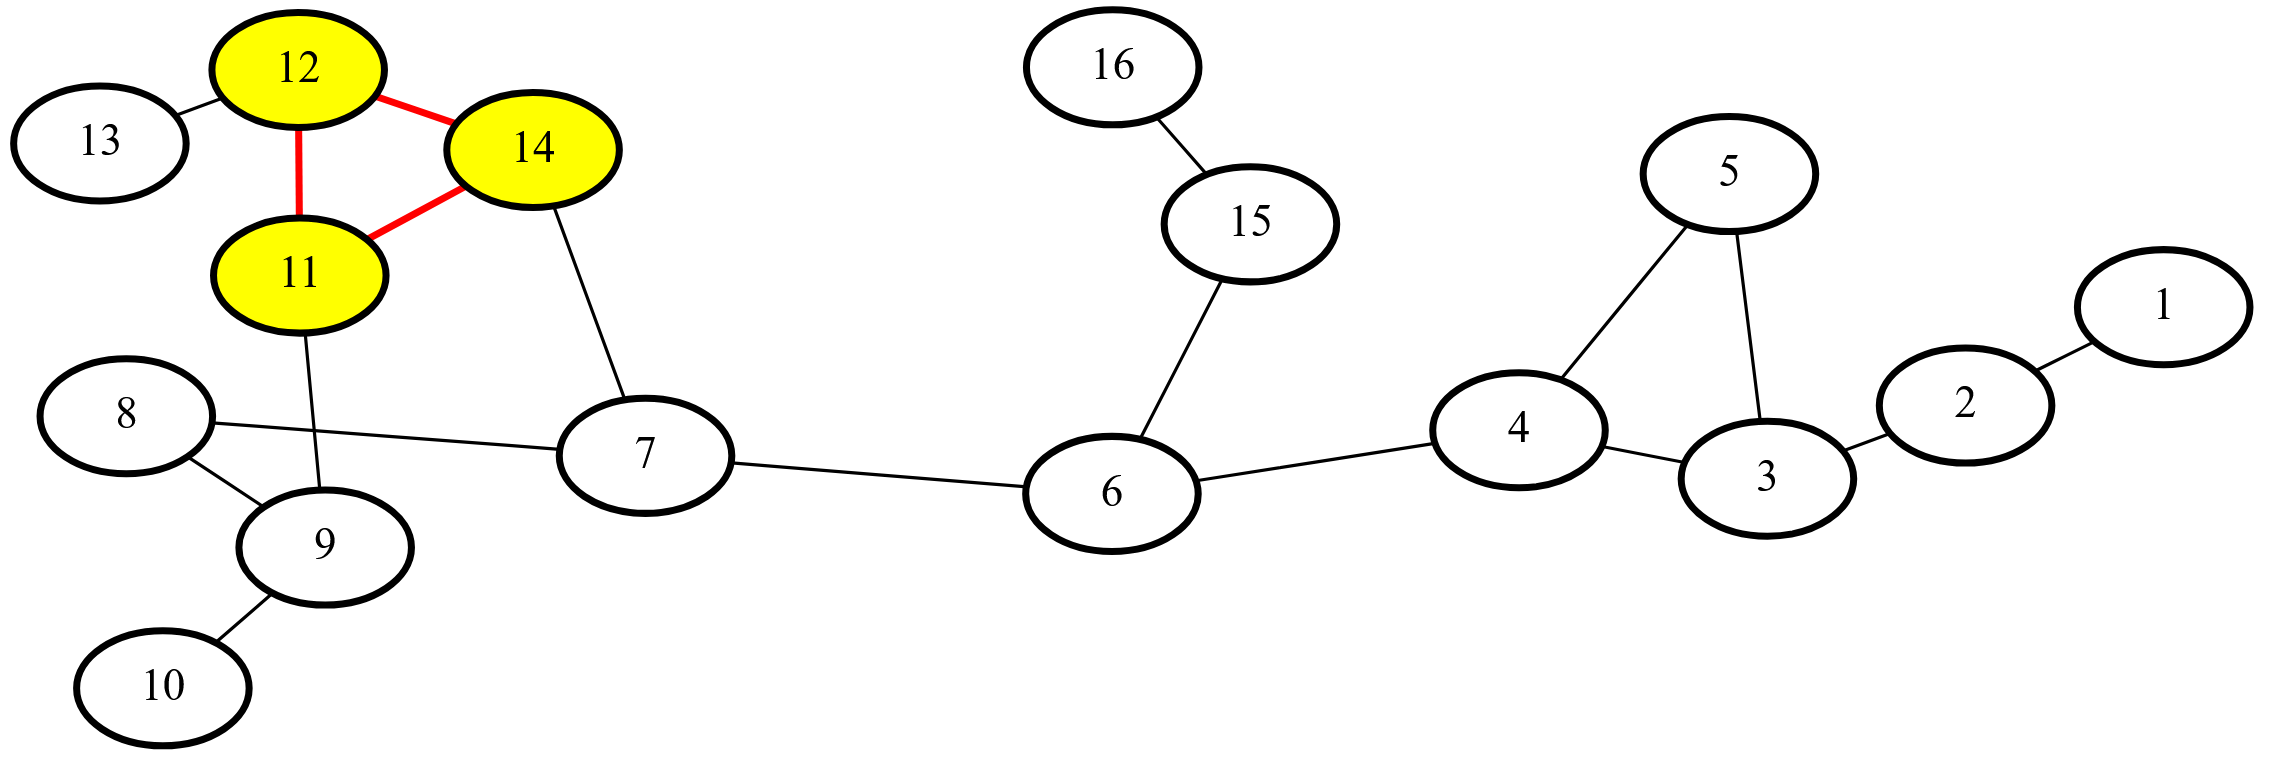
\includegraphics[width=\linewidth]{images/minvc16graph9.png}
	\caption[Graph with 16 nodes]{A graph with 16 nodes and highlights for the subgraph $\{11,12,14\}$ in yellow and red edges.}
	\label{fig:minvc16graph9}
\end{figure}

\begin{figure}[H]
	\centering
	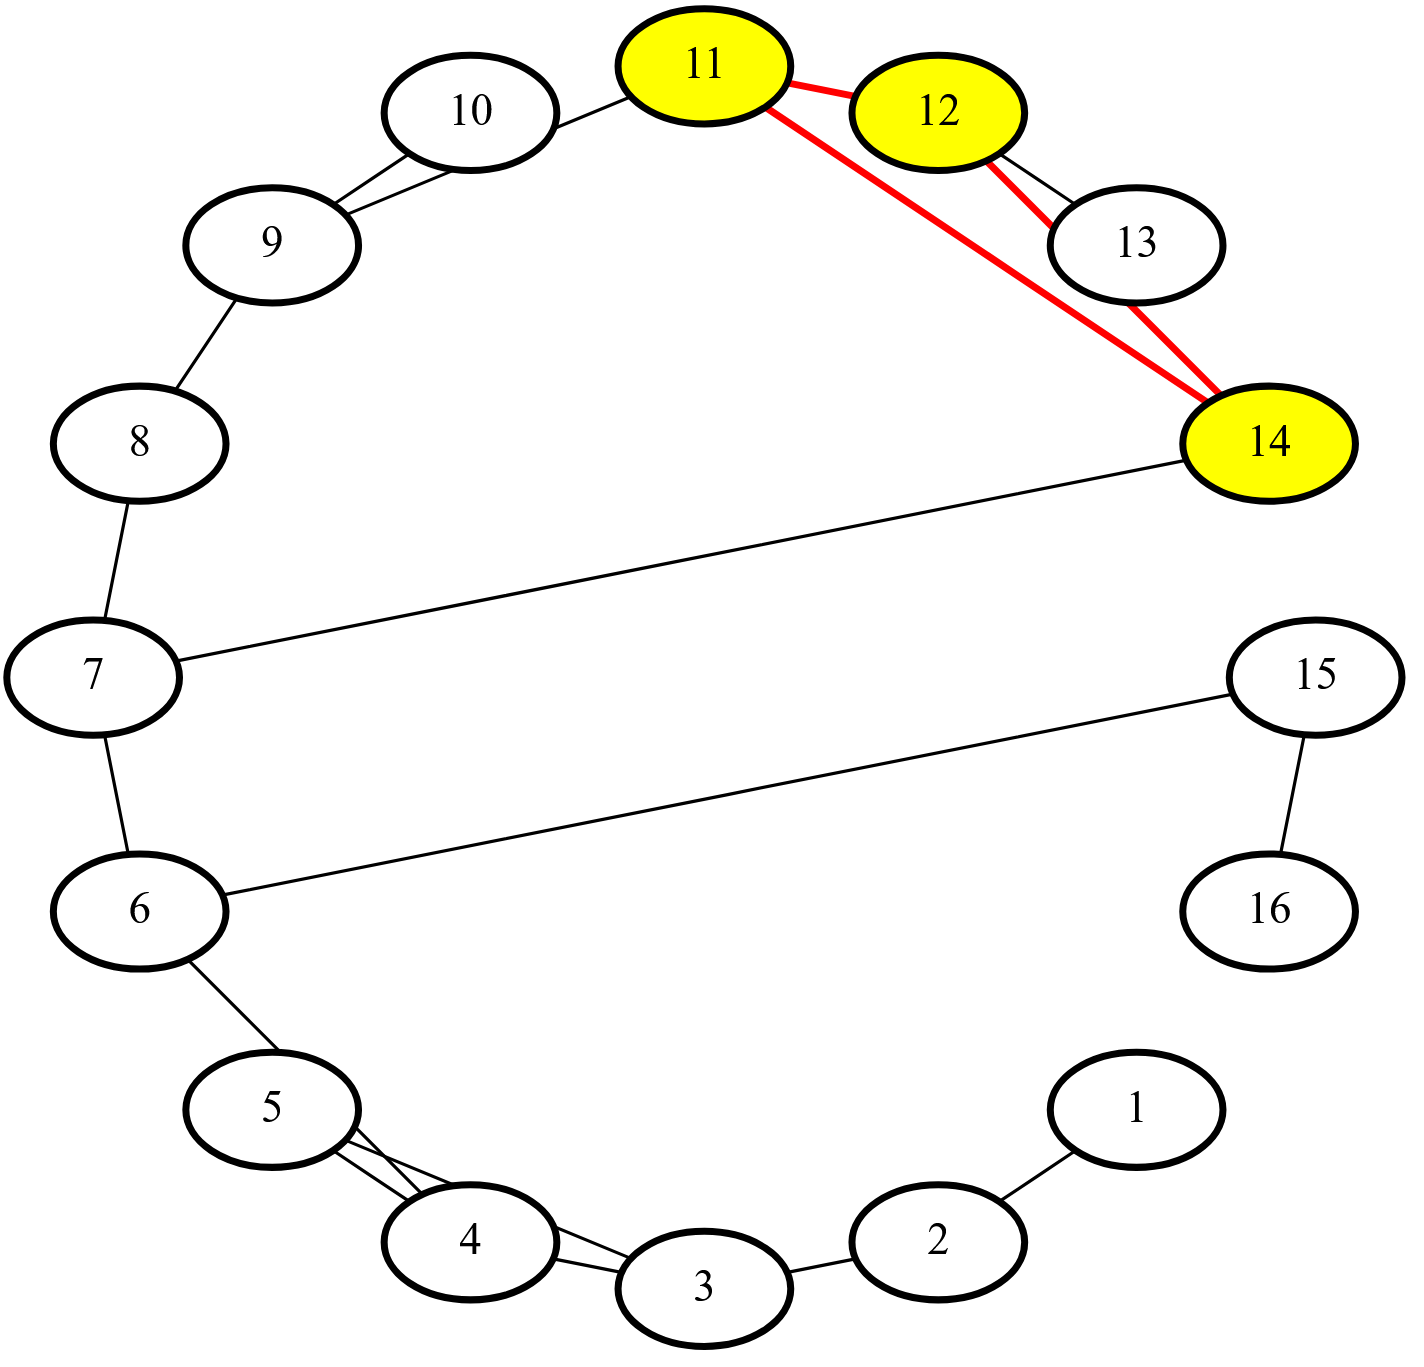
\includegraphics[width=0.6\linewidth]{images/minvc16graph9sorted.png}
	\caption[Graph with 16 nodes on a circle]{A graph with 16 nodes and highlights for the subgraph $\{11,12,14\}$ in yellow and red edges. The nodes are arranged in a circular layout and sorted by their labels from 1 to 16.}
	\label{fig:minvc16graph9sorted}
\end{figure}

%============== Joining SVG ====================================================
\subsection{Joining SVG}\label{sec:svgjoin}
Once all user defined images for one timeline are created, it would be nice to have all graphs combined in one file for each step. All created graphs for each time step together create a overall impression of the work done during solving this step. It showed to be inconvenient to manually open and view the tree decomposition along the primal, dual, incidence or fundamental graph for each time step and problem instance, so we automated this task.
 To provide some basic scaling and adjusting, we prepared a section in the API for joining the resulting SVG graphics.
Its parameters can be viewed in \textit{SvgJoinData} in Listing \ref{lst:svgjoindata} on page~\pageref{lst:svgjoindata}. \\
We have prepared some examples at the end of this section.
The currently implemented functionality could be further extended upon using SVG animations\footnote{\url{www.w3.org/TR/SVG11/animate.html}}.\\

%The functionality is placed in the file \textit{svgjoin.py} and will be called with the specifications given in the optional dictionary \textbf{svgjoin} within the JsonAPI.


% Show example with description of parameters 
%The internally used method \textit{svgjoin.append\_svg} joins two images horizontally in each step.
With the default settings, it aligns the top edge of both images and applies no scaling to either image.
The four parameters, each with its expected type and default value in Table~\ref{tab:svgjoin} allow flexible \textbf{vertical}, \textbf{horizontal} and \textbf{scaling} transformations.
\begin{table}[h]
	\centering
	\begin{tabular}{|lllc|}
		
		\hline
	   parameter& type & default & unit\\
		\hline\hline
		 padding& int & 0&  image coordinates\\
		 
		  v\_bottom& float & None & size of the \textit{first} image\\
		  
		  v\_top& float & None & size of the \textit{first} image\\
		  
		 scale2& float & 1 & size of the \textit{second} image\\
		 
		 \hline\hline
	\end{tabular}
	\caption{The four parameter allowing free transformations when joining images.}\label{tab:svgjoin}
\end{table}

Note that the images are placed in a Cartesian coordinate system and their origin is the upper left corner of their bounding box. All images fill a rectangle in this coordinate system with height and width respectively.
Since the order of the parameters \textit{v\_bottom} and \textit{v\_top} could be confused due to the inverted y-axis, we make sure that \textit{v\_top} is correctly set to the smaller and \textit{v\_bottom} to the larger value whenever possible.

A special case is obtained by setting both parameters \textit{v\_bottom} and \textit{v\_top} to the same number. Then they are interpreted as the position of the vertical centerline for the second image in units of the first. So setting both parameters to $\frac{1}{2}$ would result in both images being vertically centered.\\

If we want to position more than two images, it is possible to specify the parameters in a list.
The list can be of different length for each parameter - if it is exhausted, the last parameter in the list will be repeatedly used until all images are joined together.

%==============================================================================
%============== GPUSAT ========================================================
%==============================================================================

\section{Integration in gpusat}\label{sec:gpusat}
%To study and improve the handling of the C++ program was chronologically the first task we experimented with.
%Getting the program up and running proved to be more difficult than we envisioned due to a probable bug in the driver when running OpenCL Drivers from CUDA on the Windows OS.

The integration of visualization into the C++ based \url{github.com/daajoe/GPUSAT} did happen in two parts. \\
The first part is mostly included in the class \textit{Graphoutput}, and includes several experimental steps into visualization. This class has 186 lines of code (LOC) in its source file, and 44 lines of code in its header file.

The second part was done in the class \textit{Visualization}, and fulfills the API to \textit{tdvisu}. This class consists of 203 LOC in its source file, and 86 LOC in its header file.

The integration into the existing classes from \textit{gpusat} is listed in Tab.~\ref{tab:loc}. 
\begin{table}[h]
	\centering
	\begin{tabularx}{0.4\textwidth}{|Y|c|c|}
		\hline
		{\centering gpusat} & main & Solver \\
		\hline\hline
		Graphoutput & 6 & 10 \\
		\hline
		Visualization & 5 & 7 \\
		\hline\hline
		
	\end{tabularx}
		\caption[LOC needed for implementation of visualization in \textit{gpusat}]{Lines of code referencing the classes Graphoutput and Visualization \\
			from the main-method or the Solver class.}\label{tab:loc}
\end{table}


%=================Performance=======================
%Impact on performance:
With utilizing {streams}\footnote{\url{www.cplusplus.com/reference/sstream/stringstream}} for all string operations we tried to keep the impact on performance during the solving process small. When running on the same thread, especially for larger problem instances, the creation of the visualization files could impact the performance of the run. With the relatively small examples we used to visualize during our development process this was not noticeable.

%Some non-functional changes made to the source were 
%\begin{itemize}
%	\item[a)] some adjustments to satisfy the local compiler (shortening kernel string, replacing '\emph{and}' with '\&\&')
%	\item[b)] some explicit casts
%	\item[c)] fixed documentation of command line arguments
%\end{itemize}
%
%The functional changes were:
%\begin{enumerate}
%	\item allow tabs instead of spaces in input files
%	\item output more information about the hardware used (device\_query)
%	\item add verbose output globally toggled by a flag 
%	\item decide on \url{en.wikipedia.org/wiki/DOT_\%28graph_description_language\%29} 
%		as the intermediate format for storing graphs.
%	\item start collecting information that might be needed for a visualization
%		\emph{graphfile} for saving the decomposition graph
%	\item add \emph{graphout }to solver flow to get automated insight into the structure of a run.
%	
%	\item add function \emph{solutiontable} to extract tables of variable assignments as a string
%	\item add labels to each node (bags and solutions at this point)
%	\item encapsulating the previous functions into gpusat::Graphoutput class and instantiate it in main.
%	\item using the class functionality in the Solver
%	\item changing enum to the \href{coders-corner.net/2017/08/13/scoped-vs-unscoped-enum/}{scoped enum class} for better encapsulation and strongly typed.
%	\item with \href{github.com/daajoe/GPUSAT/commit/cfb310}{inlining gpusatutils} the current functionality of creating raw dot was completed.
%	
%	\item Experimented with Neo4j, but found the visualization in particular not that presentable. The functionality to create \href{neo4j.com/developer/cypher-resources/}{cypher-queries} for the SAT formula with primal, incidence and dual graph is still present in the class.
%	\item The functionality to create the cypher-query for the graph of the tree-decomposition was added.
%	\item Rename \textit{visualisierung} into \textit{visualization}
%	\item Using \href{github.com/open-source-parsers/jsoncpp}{JsonCPP} for processing and formatting json objects in C++
%	\item Setting format to {BasedOnStyle: LLVM, UseTab: Never, IndentWidth: 4, TabWidth: 4, ColumnLimit: 0}
%	\item Creating a \emph{Grid} class for efficiently storing unsigned integer values in a two-dimensional structure
%	based on ideas from \href{stackoverflow.com/questions/936687}{this thread}
%	\item create \href{github.com/VaeterchenFrost/GPUSAT/blob/master/VisualCodeUsage.md}{guide} for remote development with \emph{Visual Code}
%	\item Converted intermediate string operations to string-streams instead of files
%	\item Updated README.md
%	\item Added Doxygen for docbook, html, latex	
%\end{enumerate}
The forked repository, with visualization and some minor fixes included, can be seen on \url{github.com/VaeterchenFrost/GPUSAT}. \\
The changes made when developing this integration can be seen here\footnote{\url{github.com/daajoe/GPUSAT/compare/master...VaeterchenFrost:master}}.

%Working with cmake remotly. ssh @(sg1.)dbai.tuwien.ac.at
%CPU branch wasn't working.
%Only AMD/Nvidia graphics  with respective flags.

%Manual configuration with the include options from \href{cmake.org/}{cmake} in \href{github.com/VaeterchenFrost/GPUSAT/blob/master/CMakeLists.txt}{CMakeLists.txt}
%or with help from \url{marketplace.visualstudio.com/items?itemName=ms-vscode.cmake-tools}
%to set up for the (potentially remote) environment.
%\begin{longtable}{|r|p{10cm}|}
%	\hline
%	Option & Description\\
%	\hline\hline
%
%	\endhead
%	
%-s, -{}-seed INT&  number used to initialize the pseudorandom number generator\\\hline
%	-f, -{}-formula TEXT &  path to the file containing the sat formula\\\hline
%	-d, -{}-decomposition TEXT  &   path to the file containing the tree decomposition\\\hline
%	-{}-CPU                   &    run the solver on a cpu\\\hline
%	-{}-NVIDIA                &    run the solver on an NVIDIA device\\\hline
%	-{}-AMD                   &    run the solver on an AMD device\\\hline
%	-{}-weighted              &   use weighted model count\\\hline
%	-{}-noExp                 &    don't use extended exponents\\\hline
%	-v, -{}-verbose            &    print additional program information\\\hline
%	-p, -{}-nopreprocess       &    skips the pre-processing step for debugging and visualization purposes\\\hline
%	-w, -{}-combineWidth (20) &    maximum width to combine bags of the decomposition\\\hline
%	-g, -{}-graph TEXT        &    filename for saving the decomposition graph\\\hline
%	-{}-visufile TEXT         &    filename for saving the visualization file\\\hline
%	\hline
%	\caption{Usage: ./gpusat [OPTIONS]
%		\label{tab:optionsgpusat}}
%\end{longtable}      
        
An example call with \textit{./gpusat -f ../examples/test\_da4\_1.cnf -v -p -d ../examples/td4p1.txt  -g ../examples/graphfileda41.txt -{}-visufile ../examples/visufileda41.json} enabled verbose output, disabled pre-processing to prevent the creation of bags with too many variables at once to be visualized, and creates full visualization output. 
The example console output produced by this call is included in Listing \ref{lst:outputgpusat} on page \pageref{lst:outputgpusat}.

%============== Graphoutput ====================================================
\subsection{Class Graphoutput}\label{sec:chagraphoutput}
This class does include the first steps to automatically visualize the tree decomposition of the solving process with its solutions.
Its main funcionality can output visualizations specified in gml (Graph Modeling Language)~\cite{Himsolt2010GMLAP}. We see one small example output in Listing \ref{lst:g41digraphgml} on page~\pageref{lst:g41digraphgml} with labeled nodes and two edges. The output can be seen in Figure~\ref{fig:gmlexamplepic}.
%For our example for \#SAT~\ref{lst:g41digraphdot} with the bags and respective solutions as nodes connected to the bag they solve.

\begin{figure}[h]
	\centering
	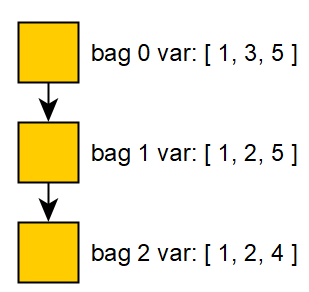
\includegraphics[]{images/gmlexamplepic.png}
	\caption[GML example plotted with yEd]{GML source from Listing \ref{lst:g41digraphgml} when plotted (\textit{layout modified}) with yEd {\url{yworks.com/products/yed} Version 3.20 powered by the yFiles Graph Visualization Library \url{www.yWorks.com}} }
	\label{fig:gmlexamplepic}
\end{figure}
Additional methods exist so we could evaluate the possibilities of using graph-databases like Neo4j~\cite{graphdatabases}.
It is possible to create visualizations of the initial situation for CNF Clauses and the computed tree decomposition of the primal graph as two \textit{Neo4j Cypher}\footnote{\url{neo4j.com/docs/cypher-refcard/current/}} queries constructing:
\begin{itemize}[label=-]
	\item one graph representing the SAT formula and queries to construct incidence, dual and primal representations in method \textit{Graphoutput::neo4jSat}
%	output as satFile = ``cypherSatFormula.txt"
	\item one graph representing the tree decomposition of the primal graph. This happens in method \textit{Graphoutput::neo4jTD}.
%	output as tdFile = ``cypherTreedec.txt"
\end{itemize}

While these representations can be helpful in visualizing small parts of the results using the tools available, we did prefer more direct access to the layout and style via the methods described in this thesis.\\
It  should be noted that this can be useful in interactively querying properties of the results, something that our current solution using DOT and SVG as output does not provide.

%============== Visualization ====================================================
\subsection{Class Visualization}

The integration with the API of \textit{tdvisu} is handled by this class.
To help with the creation of valid \textit{JSON} we used the c++ library JsonCpp~\footnote{\url{github.com/open-source-parsers/jsoncpp} version 1.9.2}  from the open-source-parsers repository. 

\medskip\noindent
This class provides the generation of the required parts for the schema with only little customization. The reader is welcome to add optional parts of the schema on the basis of the existing implementation.
We provide the API with the basic incidence graph specification and request that the primal graph is computed from it. The tree decomposition, as well as the timeline of the solver, is also added without special configuration.

We call its method \textit{Visualization::tdTimelineAppend} six times in the solver with different parameters according to the state in which the solver is currently in.

From the main method of \textit{gpusat} we call its constructor, as well as its methods \textit{visuClauses} to create the incidence graph and \textit{visuTreeDec} to provide the tree decomposition for the visualization. After the solving process is finished, the method \textit{writeJsonFile} is called to write the result on the disk.

%==============================================================================
%============== DPDB ==========================================================
%==============================================================================

\section{Integration in dpdb}\label{sec:dpdb}
{Dpdb} as a project provides a framework that allows many different problems to be solved using dynamic programming on TDs. It utilizes relational databases, and currently provided reference implementations for the problem types SAT, \#SAT and MinVC, one which is not implemented in \textit{gpusat}.
The integration of the API with dpdb is only minimally invasive when implemented after the solving process instead of running parallel to the solver. 
The only interference to the solving process is, that all necessary information has to be persisted in the database.
The integration is included in our \textit{tdvisu} project as a separate Python file.
A complete workflow was accomplished using the arguments
\begin{itemize}
	\item -{}-store-formula as a problem specific option for Sat and SharpSat
	\item -{}-gr-file GR\_FILE for problems like VertexCover with graph input 
\end{itemize}
when calling \textit{dpdb.py}.\\
Our program consists of the file \textit{construct\_dpdb\_visu.py} with the PostgreSQL database adapter Psycopg\footnote{\url{www.psycopg.org}} and few additional internal dependencies.

Its command to collect the needed data for visualization after a \textit{dpdb} run accepts the following flags:
\begin{itemize}
	\item
	\textbf{problemnumber},
	 the problem-id to select in the database
	 
	\item
	\textbf{-{}-twfile }\textit{TWFILE},
	tw-file containing the edges of the graph 
	
	\item
	\textbf{-{}-outfile }\textit{OUTFILE},
	 file to write the output to, default 'dbjson\%d.json'
	 
	\item
	\textbf{-{}-loglevel }\textit{LOGLEVEL},
	 set the minimal loglevel for the root logger
	 
	\item
	\textbf{-{}-pretty},
	 pretty-print the JSON
	 
	\item
	\textbf{-{}-inter-nodes}
	Calculate and animate the shortest path between successive bags in the order of evaluation. 
%	To accomplish this task, an efficient implementation of the bidirectional Dijkstra's algorithm \cite{shortestPathAlgo} based on the implementation by NetworkX \cite{SciPyProceedings_11} in {bidirectional\_dijkstra}\footnote{\url{networkx.github.io/documentation/networkx-2.1/\_modules/networkx/algorithms/shortest\_paths/weighted.html\#bidirectional\_dijkstra}} was adapted.
%	In our use case the weight function is always one, as the edges have no weight associated with them.
\end{itemize}
%After the arguments are parsed by \href{docs.python.org/3/library/argparse.html}{Pythons argparse} it is possible to adjust logging output by either providing a configuration file (\href{github.com/VaeterchenFrost/tdvisu/blob/master/tdvisu/logging.yml}{template} provided) or giving a minimal logging level per program argument.

%Next the \textit{create\_json}~\ref{lst:create-json} function connects to the database driver with the number of the stored problem. 
While we only input the number of the run stored in the database, the value ``problem type" is available as a string in its table \emph{public.problem}, and the appropriate class to prepare the data will be instantiated. Currently the solver handles the problems of \textit{satisfiability} (Sat), \textit{count solutions to a Boolean formula} (SharpSat) as well as \textit{minimum vertex cover} (VertexCover).
For further details on the implementation we refer the reader to the source code in \textit{tdvisu}\footnote{\url{github.com/VaeterchenFrost/tdvisu/blob/master/tdvisu/construct_dpdb_visu.py}}.

%==============================================================================
%============== APPLICATION ===================================================
%==============================================================================
\newpage
\section{Application and Images}\label{sec:appl}

% Appl. Sat
\subsection{SAT Example}\label{sec:applsat}
As a first complete visualization output we show the full output of checking the Boolean formula (Example \ref{ex:example41} in Chapter \ref{sec:BSP}) for solvability. We have six time steps included in this run. First we will look at the bags in the tree-decomposition, where as simple debugging information we added the time to solve each bag individually into the labels. See Fig. \ref{fig:DA4SAT_TDStep1}, Tab. \ref{tab:DA4SAT_TDStep2345} and Figure \ref{fig:DA4SAT_TDStep6}.  We see the nodes gathered in each bag as an array indicated in the TD. The solver goes from bottom to top through the bags. The active bag in each step is indicated by its changing color. When a solution was found, it gets connected as a new node by an edge to its bag. The order the bags got solved is 5, 4, 3, 2 and 1. The last solution added, containing more than zero (partial) assignments in Fig. \ref{fig:DA4SAT_TDStep6}, provides the answer ``yes" to the question of SAT.

\begin{figure}[H]
	\centering
	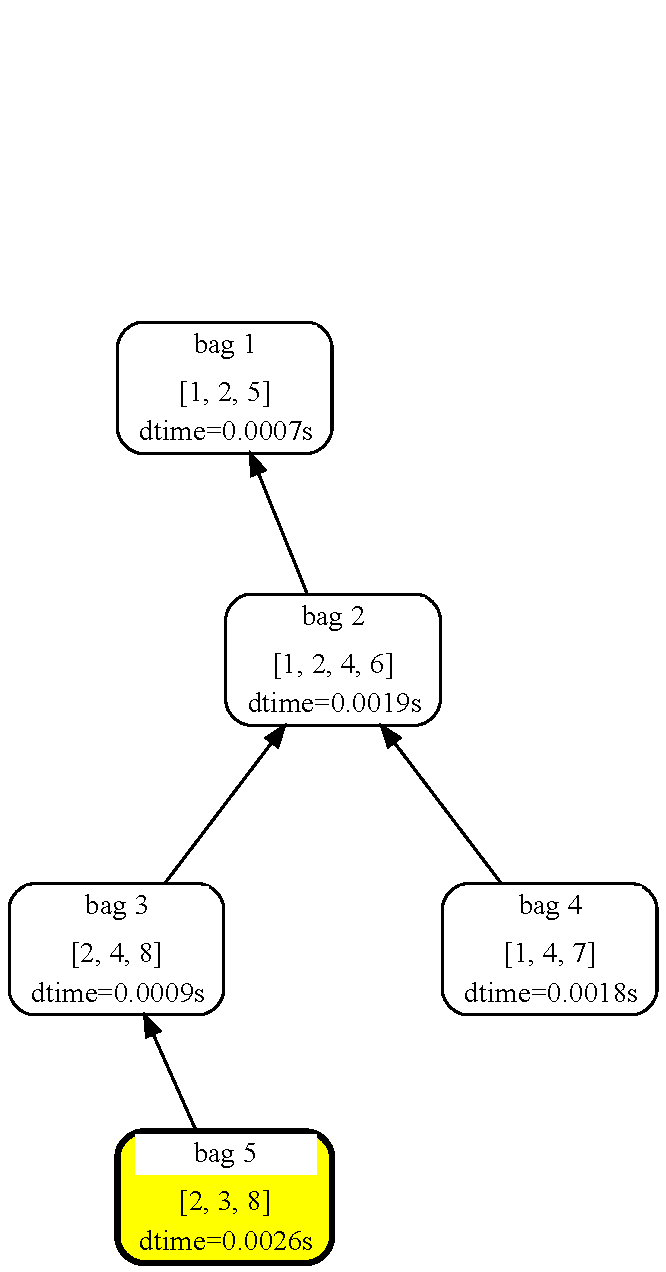
\includegraphics[height=0.5\textheight]{images/DA4SAT/results/TDStep1.pdf}
	\caption[Tree decomposition for SAT step one]{Tree decomposition for solving Example \ref{ex:example41}. \\
		We see a yellow highlighting for the first leaf (bag 5) to solve.}
	\label{fig:DA4SAT_TDStep1}
\end{figure}
\begin{table}\sffamily
\begin{tabular}{l*3{c}}

	2 & 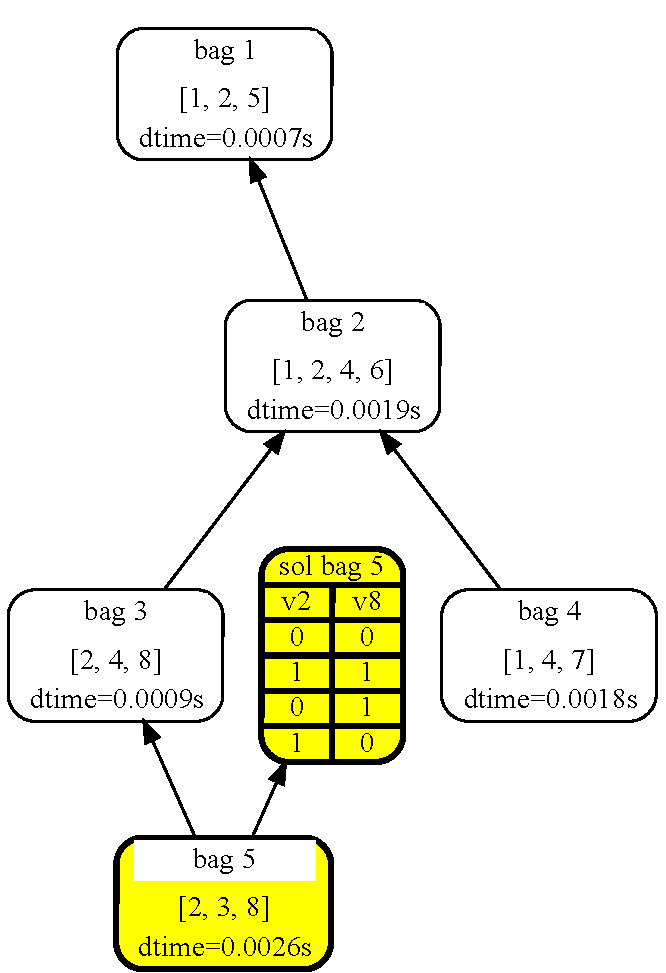
\includegraphics[height=0.46\textheight]{images/DA4SAT/results/TDStep2.pdf} &
	3 & 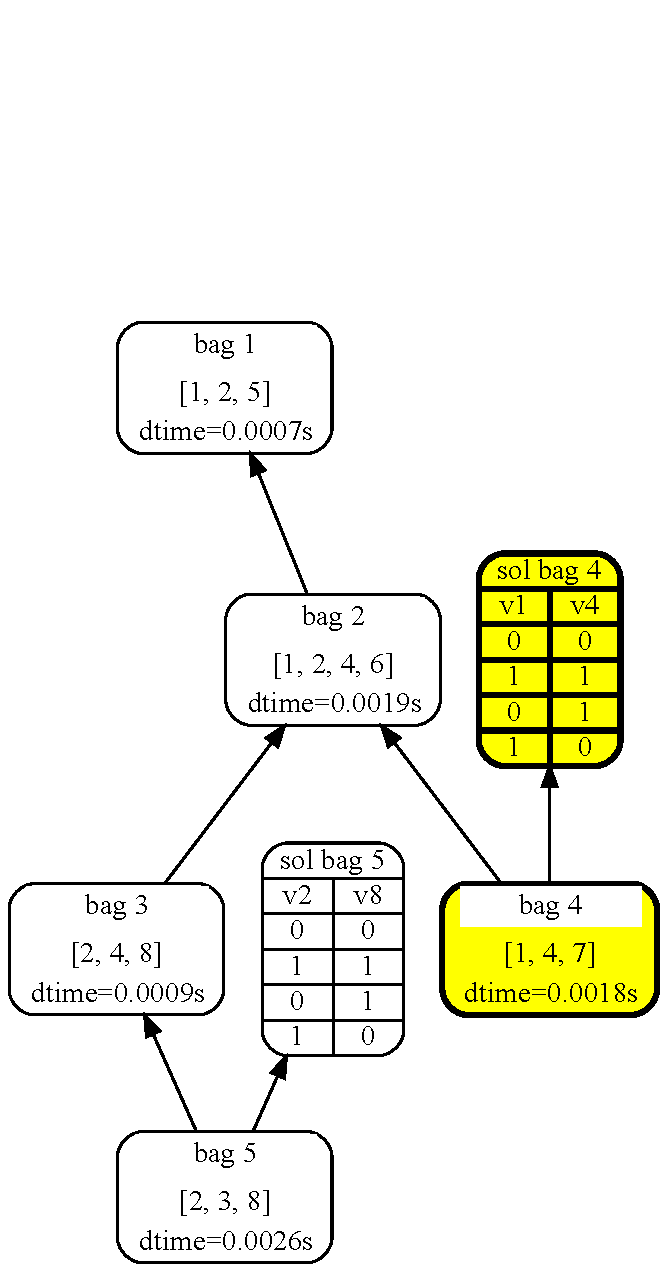
\includegraphics[height=0.46\textheight]{images/DA4SAT/results/TDStep3.pdf} \\ 
	\midrule
	4 & 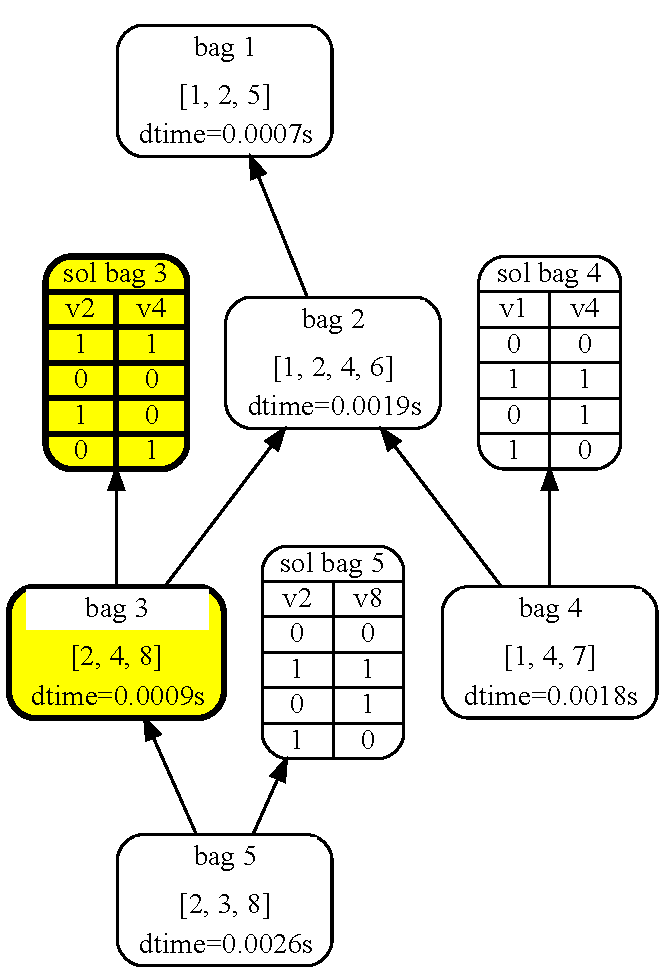
\includegraphics[height=0.46\textheight]{images/DA4SAT/results/TDStep4.pdf} &
	5 & 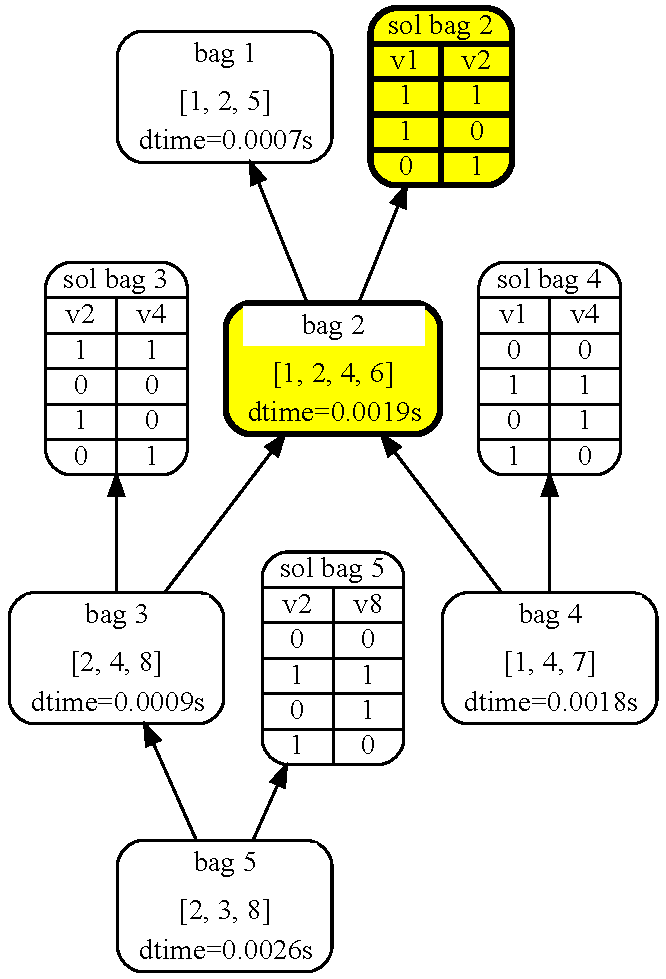
\includegraphics[height=0.46\textheight]{images/DA4SAT/results/TDStep5.pdf}\\
	\bottomrule 
\end{tabular}
\caption[Tree decomposition for SAT, steps 2-5]{Tree decomposition for solving example \ref{ex:example41} . Images for steps two to five as labeled from top left to bottom right.}
\label{tab:DA4SAT_TDStep2345}
\end{table} 

\begin{figure}[H]
	\centering
	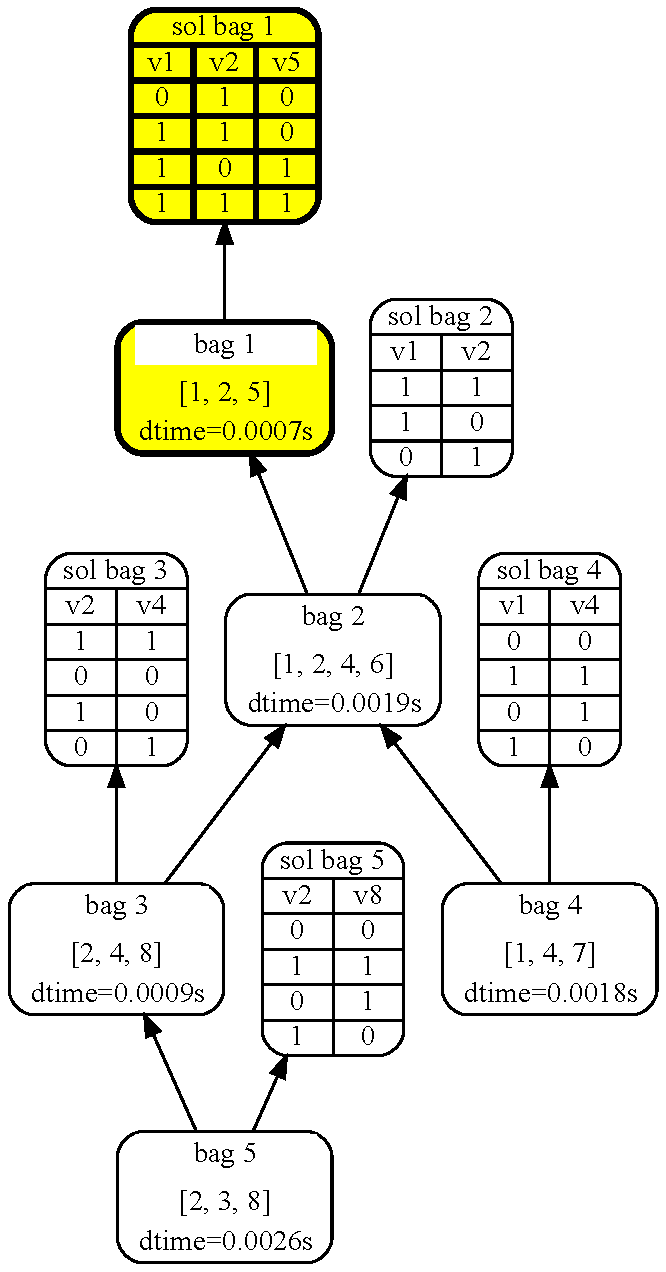
\includegraphics[height=0.6\textheight]{images/DA4SAT/results/TDStep6.pdf}
	\caption[Tree decomposition for SAT final result]{Tree decomposition for solving example \ref{ex:example41} . \\
		Final result with yellow highlighting for the last bag (1) solved.}
	\label{fig:DA4SAT_TDStep6}
\end{figure}
\medskip\noindent
In the Figures~\ref{fig:DA4SATadditional}~and~\ref{fig:DA4SATadditional2} we see the first two visualizations for incidence and primal graph with highlights corresponding to the same run as before. The first step has no highlighting. One could compare the processed Boolean formula indicated with the clauses as nodes sorted on the left-hand side. The edges either are solid lines or starting with a little circle that indicates the negation of the connected variable at the right-hand side in this clause. The nodes in the variables have three ``states". As this run operated on the primal graph, there are only variables collected in the bags. When calculating the solutions we do however need whole clauses to be processed together, so additional variables are emphasized. The three states are 1)\textit{ not included} in any clause needed, 2)\textit{ indirectly included} emphasized with a dotted border and yellow highlighting in the incidence graph, and 3) \textit{ directly included} in the bag emphasized in yellow and solid border. \\
The primal graph is also calculated directly from the Boolean formula and shows one of the same three states for each variable in its own layout.
\begin{figure}[h]
	\setkeys{Gin}{width=\linewidth,height=0.55\textheight,keepaspectratio}
	\begin{tabularx}{\textwidth}{X X }
		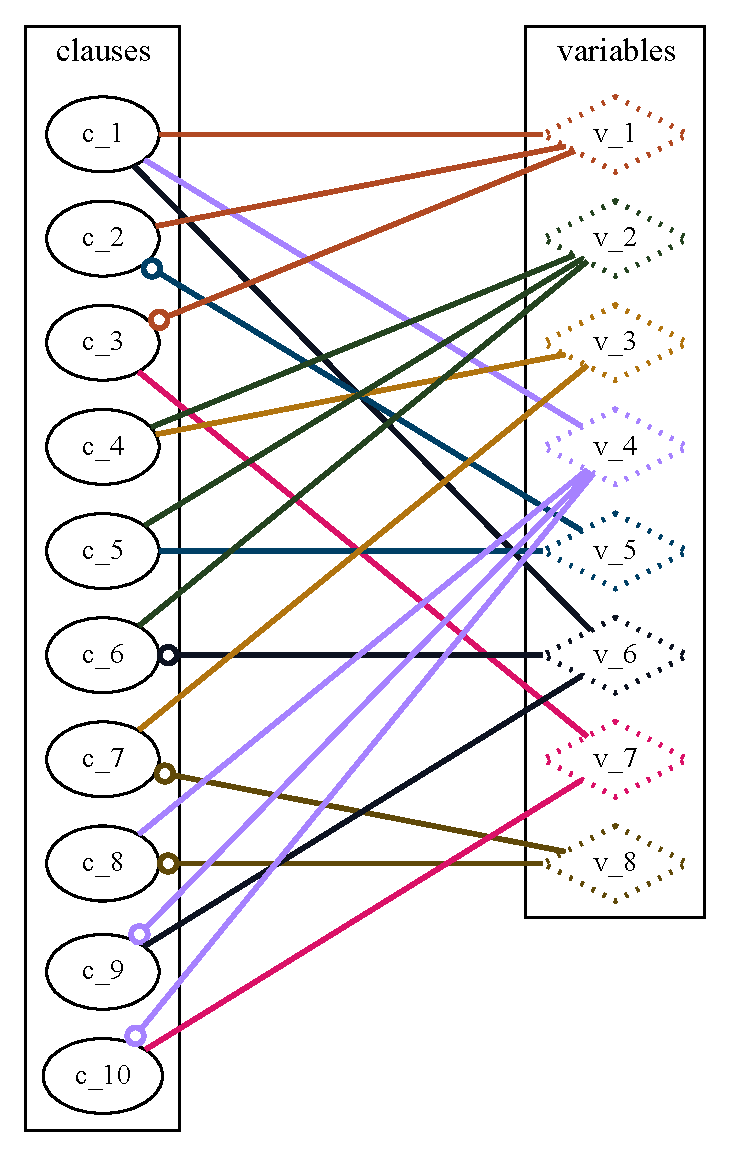
\includegraphics[valign=c]{images/DA4SAT/results/IncidenceGraphStep1.pdf} & 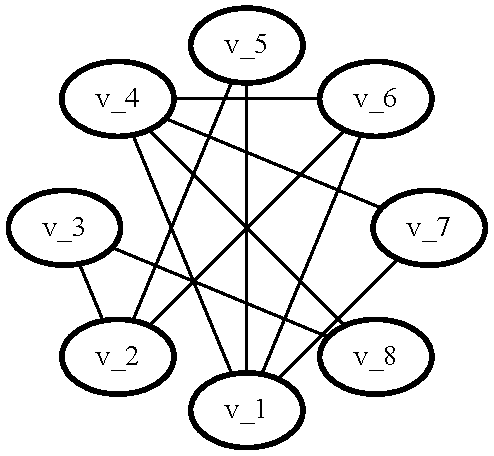
\includegraphics[valign=c]{images/DA4SAT/results/PrimalGraphStep1.pdf}
	\end{tabularx}
	\caption[Incidence graph and primal graph of Example~\ref{ex:example41}]{Incidence graph (left) and primal graph of Example~\ref{ex:example41}.}
	\label{fig:DA4SATadditional}
\end{figure}
\begin{figure}[h]
	\setkeys{Gin}{width=\linewidth,height=0.55\textheight,keepaspectratio}
	\begin{tabularx}{\textwidth}{X X }
		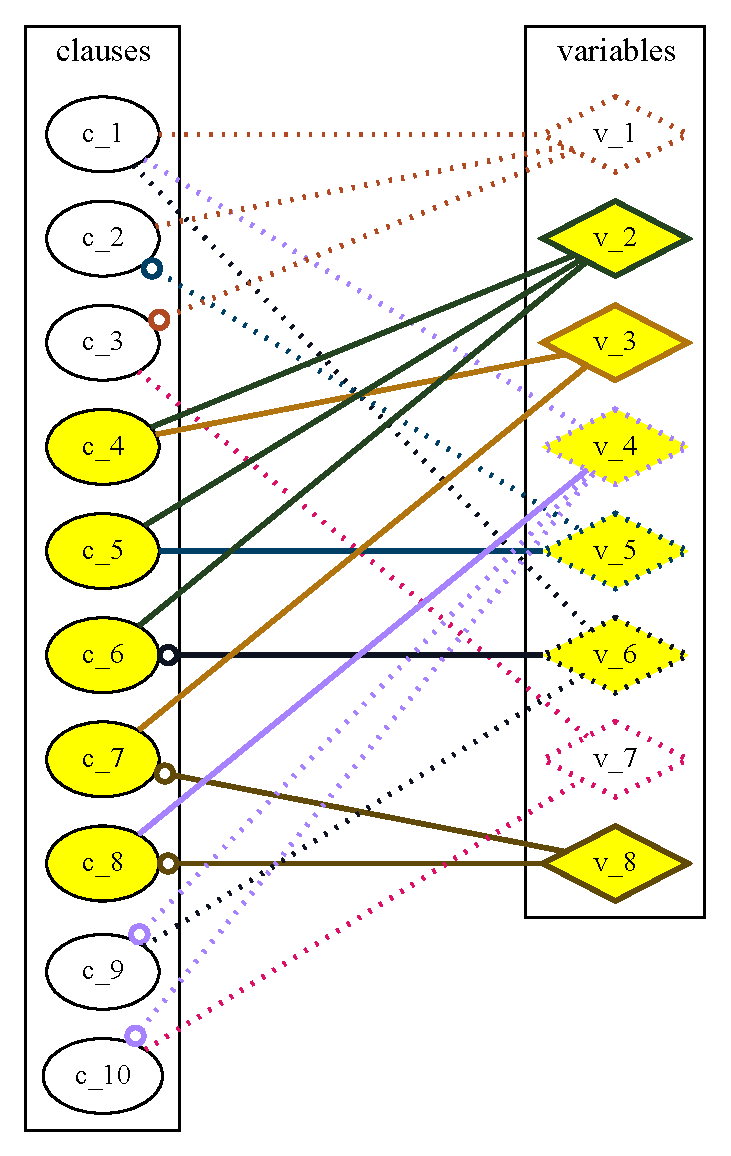
\includegraphics[valign=c]{images/DA4SAT/results/IncidenceGraphStep2.pdf} & 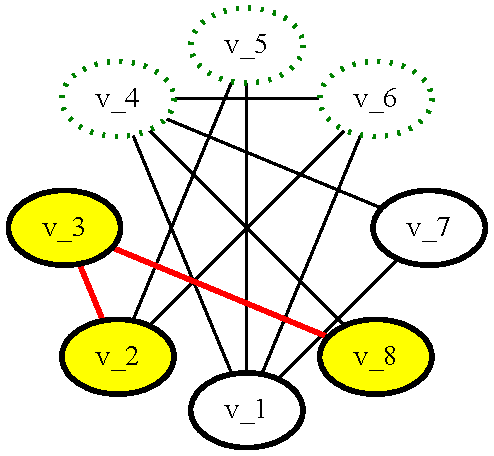
\includegraphics[valign=c]{images/DA4SAT/results/PrimalGraphStep2.pdf} 
	\end{tabularx}
	\caption[Highlighting of some parts of incidence and primal graph of Example~\ref{ex:example41}]{ Highlighting of some parts of incidence graph (left) and primal graph of Example~\ref{ex:example41}.}
	\label{fig:DA4SATadditional2}
\end{figure}
\newpage
% Appl. SharpSat
\subsection{\#SAT Example}\label{sec:applssat}
Like the previous example section we are interested in solutions to example \ref{ex:example41}. This time we want to solve \#SAT and count the number of solutions, that is the number of satisfying assignments. While the tree decomposition and SAT formula stay the same, the solver added one column to our solution-tables and label this column \textit{mc} for "\textit{model-count}", compared to pure SAT solving. It also included a footer with the API to display the sum of all models considered up to this bag. We see two time steps, beginning and end of the run, in Figures~\ref{fig:DA4TDStep2}, \ref{fig:DA4TDStep6}. Again, the empty top of the reserved space is cut out of the images compared to the direct output.
\begin{figure}[H]
	\centering
	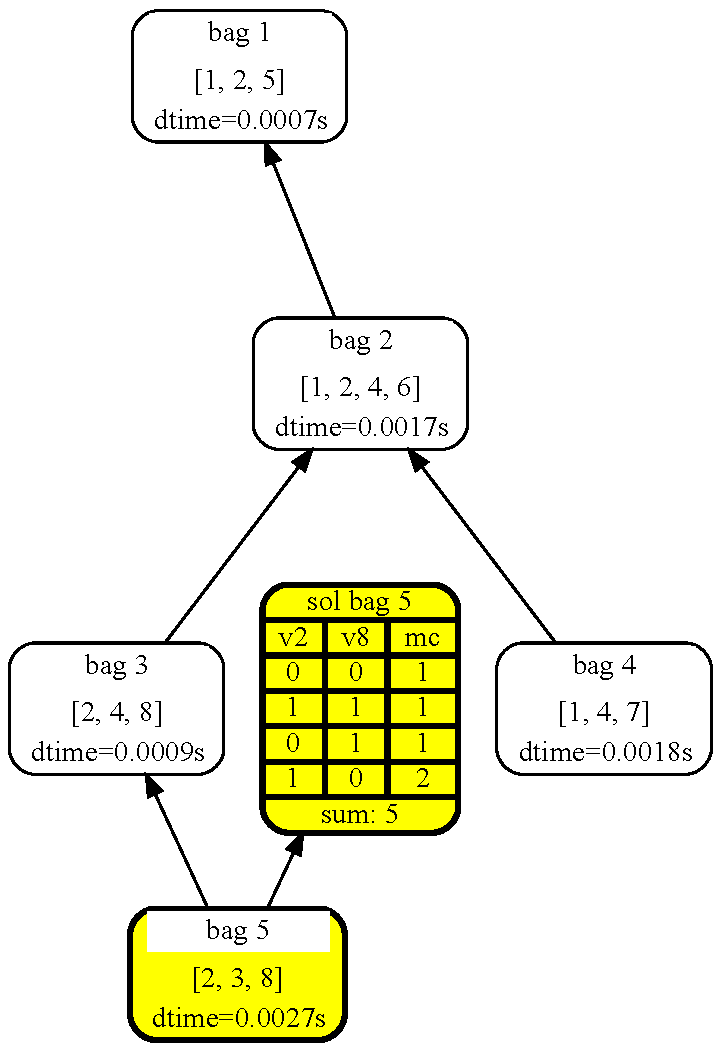
\includegraphics[height=0.6\textheight]{images/DA4/TDStep2.pdf}
	\caption[TD for \#Sat with highlighting]{Tree decomposition for solving example \ref{ex:example41} with yellow highlighting of the solution for the first leaf.}\label{fig:DA4TDStep2}
\end{figure}
\begin{figure}[H]
	\centering
	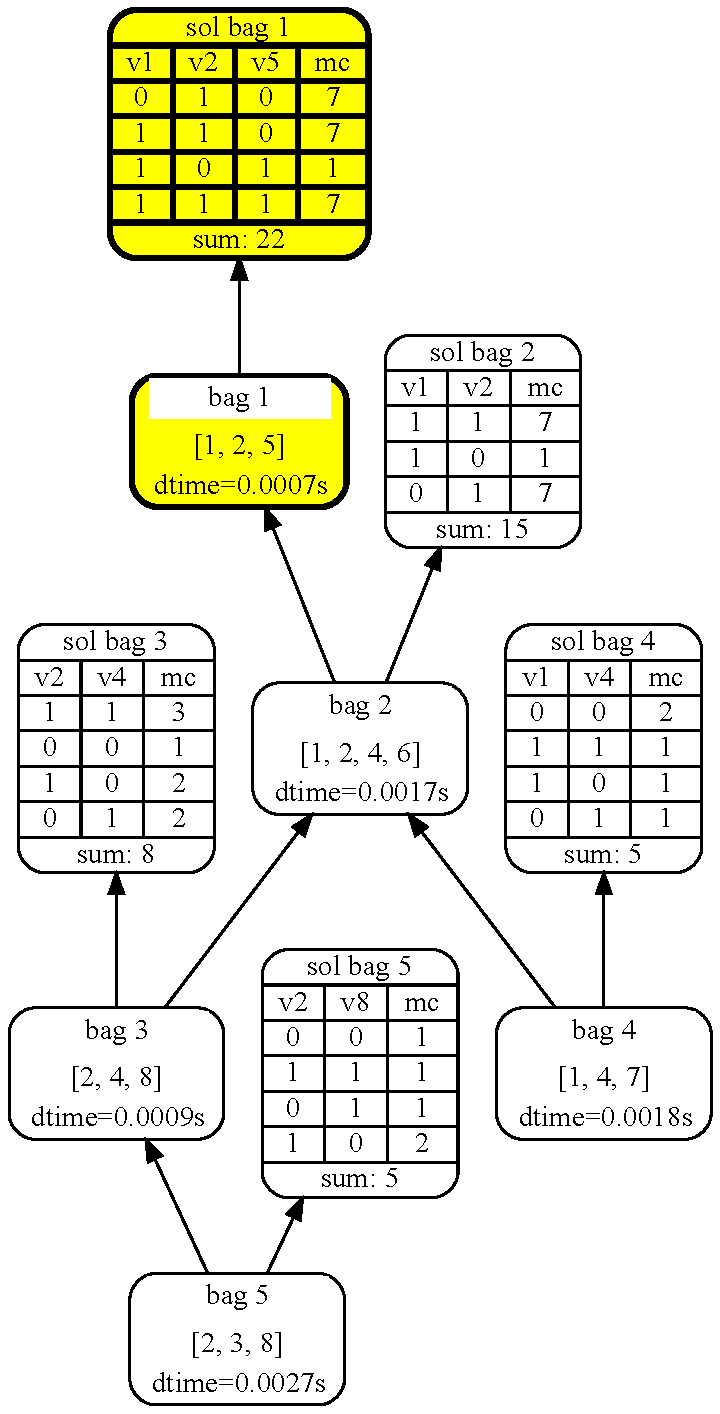
\includegraphics[height=0.9\textheight]{images/DA4/TDStep6.pdf}
	\caption[Result on TD for \#Sat]{Tree decomposition for solving example \ref{ex:example41}. The highlighted bag 1 points to the solution of the problem, containing 22 solutions and satisfying variable assignments for $v_{1},v_{2},v_{5}$ contained in \textit{sol bag 1}.}\label{fig:DA4TDStep6}
\end{figure}
% Appl. VC

\subsection{Vertex Cover Example}\label{sec:minvc}

After showing solutions around Boolean formulas, this chapter discusses a problem that is itself formulated directly on a graph.
As a very small example we will try to solve \textit{minimal vertex cover} for the following graph in Figure \ref{fig:wheelgraph} with edges seen in Listing \ref{lst:wheelgraph}.
%
%Vertex Cover Problem: For a given input graph $G=(V,E)$, a \textit{vertex cover} is a set $C$ of vertices $C \subseteq V$ so that we have $\{u,v\} \cap C \neq \emptyset$ for each edge $\{u,v\}\in E$. The problem \textit{minimal vertex cover} asks to find the minimum cardinality among all vertex covers, i.e. $|C|$ is such that there is no vertex cover $C'$ with $|C'| < |C|$.

%An instance $G=(V,E)$ of \textit{minimal vertex cover} parameterized by treewidth \textit{tw} can be solved in time $\mathcal{O}(2^{tw(G)}|V|)$ \cite{HenningParamAlgo}.

For details on the algorithms used by the solvers see also \cite[Ch. 4.2]{dpdbpadl2020} on MinVC and its Listing 3 for a template for general problems.


\begin{figure}[H]
	\centering
	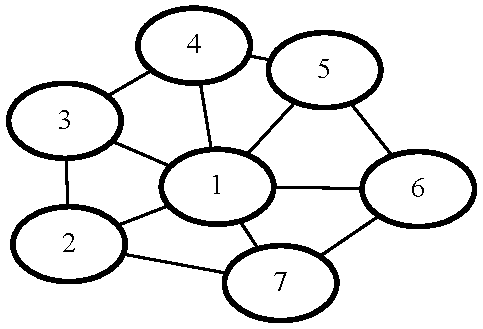
\includegraphics[]{images/WheelGraph7/graph1.pdf}
	\caption{Wheel graph with 7 vertices.}
	\label{fig:wheelgraph}
\end{figure}

The tree decomposition used created four bags with four nodes each.
The images in \ref{fig:wheelgraphc23} and \ref{fig:wheelgraphc45} are documented with the bag solved. The order here is 2, 4, 3, 1.\\
\medskip\noindent
The content in the solution nodes is very similar to the previous example on \#SAT.
The differences are the changed right-most column now reporting the size of the intermediate result if its assignment was used to cover the current graph seen up to this step. The footer now indicates the minimum of those values in each solution.
Again solving \textit{bag 1} contains the answer, this time to the question of MinVC, that the size of the minimal vertex cover is four.\\

To the right of each time step is the currently used subgraph marked with yellow nodes and red edges.


\begin{figure}[H]
	\centering
	\begin{tabular}{c}	
	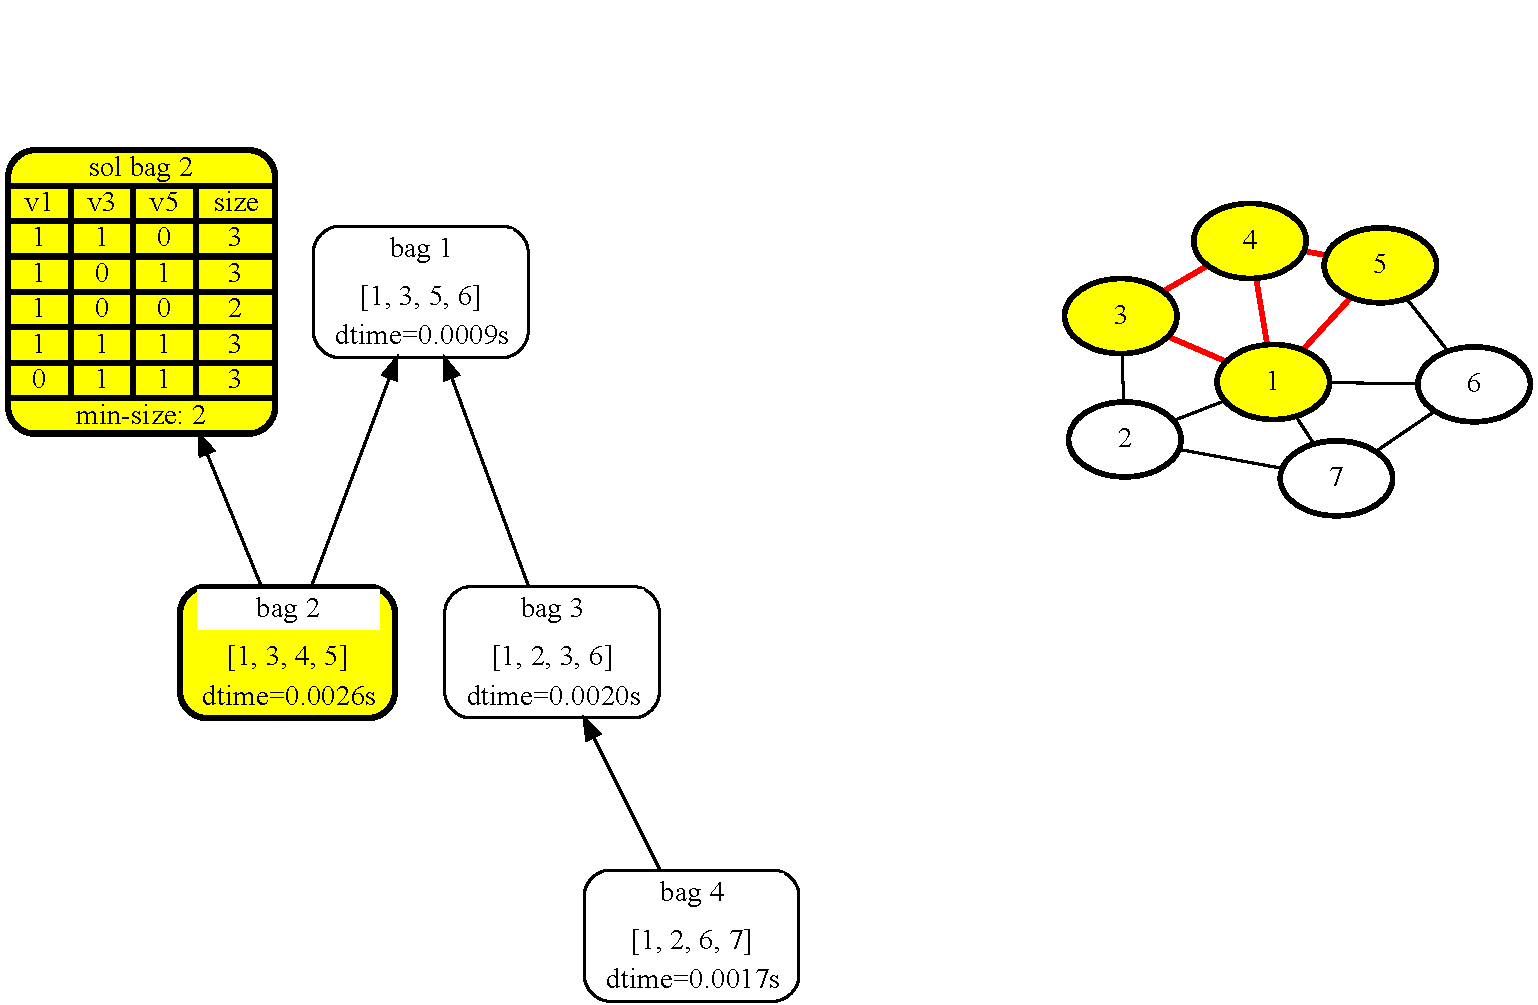
\includegraphics[width=0.99\linewidth]{images/WheelGraph7/combined2.pdf}  \\
	\hline 	\\			
		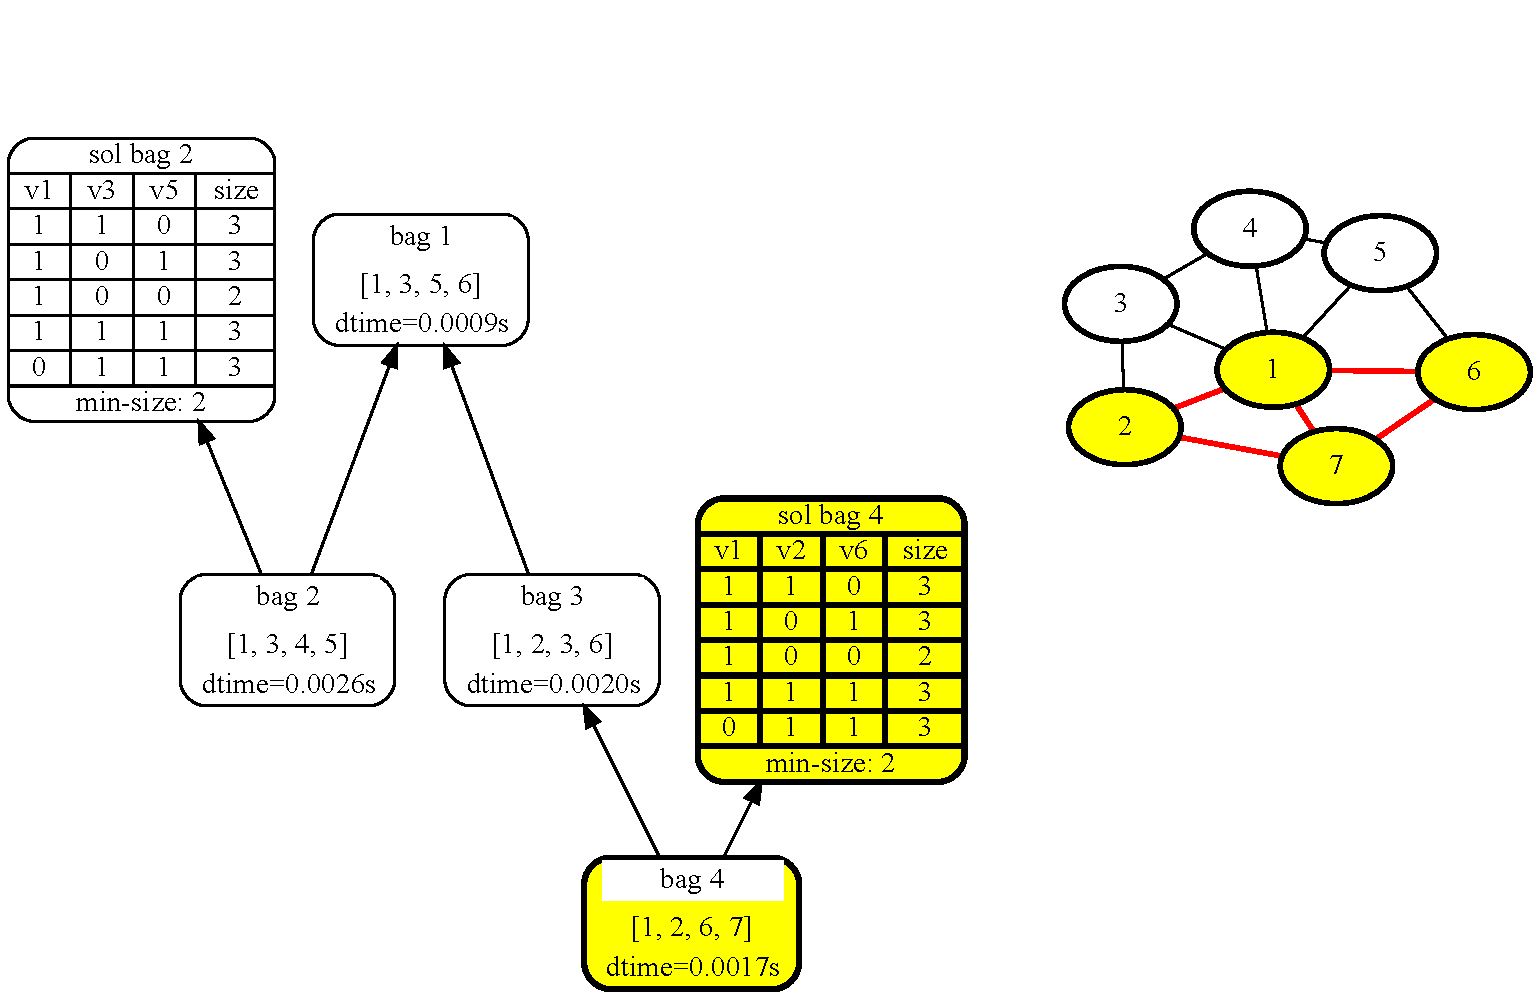
\includegraphics[width=0.99\linewidth]{images/WheelGraph7/combined3.pdf}
	\end{tabular}
	\caption[First steps to solve \textit{minimal vertex cover} for example graph \ref{fig:wheelgraph}]{First steps to solve \textit{minimal vertex cover} for example graph \ref{fig:wheelgraph} on its TD. On the top we see the first step solving \textbf{bag 2}. The lower image shows the second step solving \textbf{bag 4}.}
	\label{fig:wheelgraphc23}
\end{figure}
\begin{figure}[H]
	\centering
	\begin{tabular}{c}
		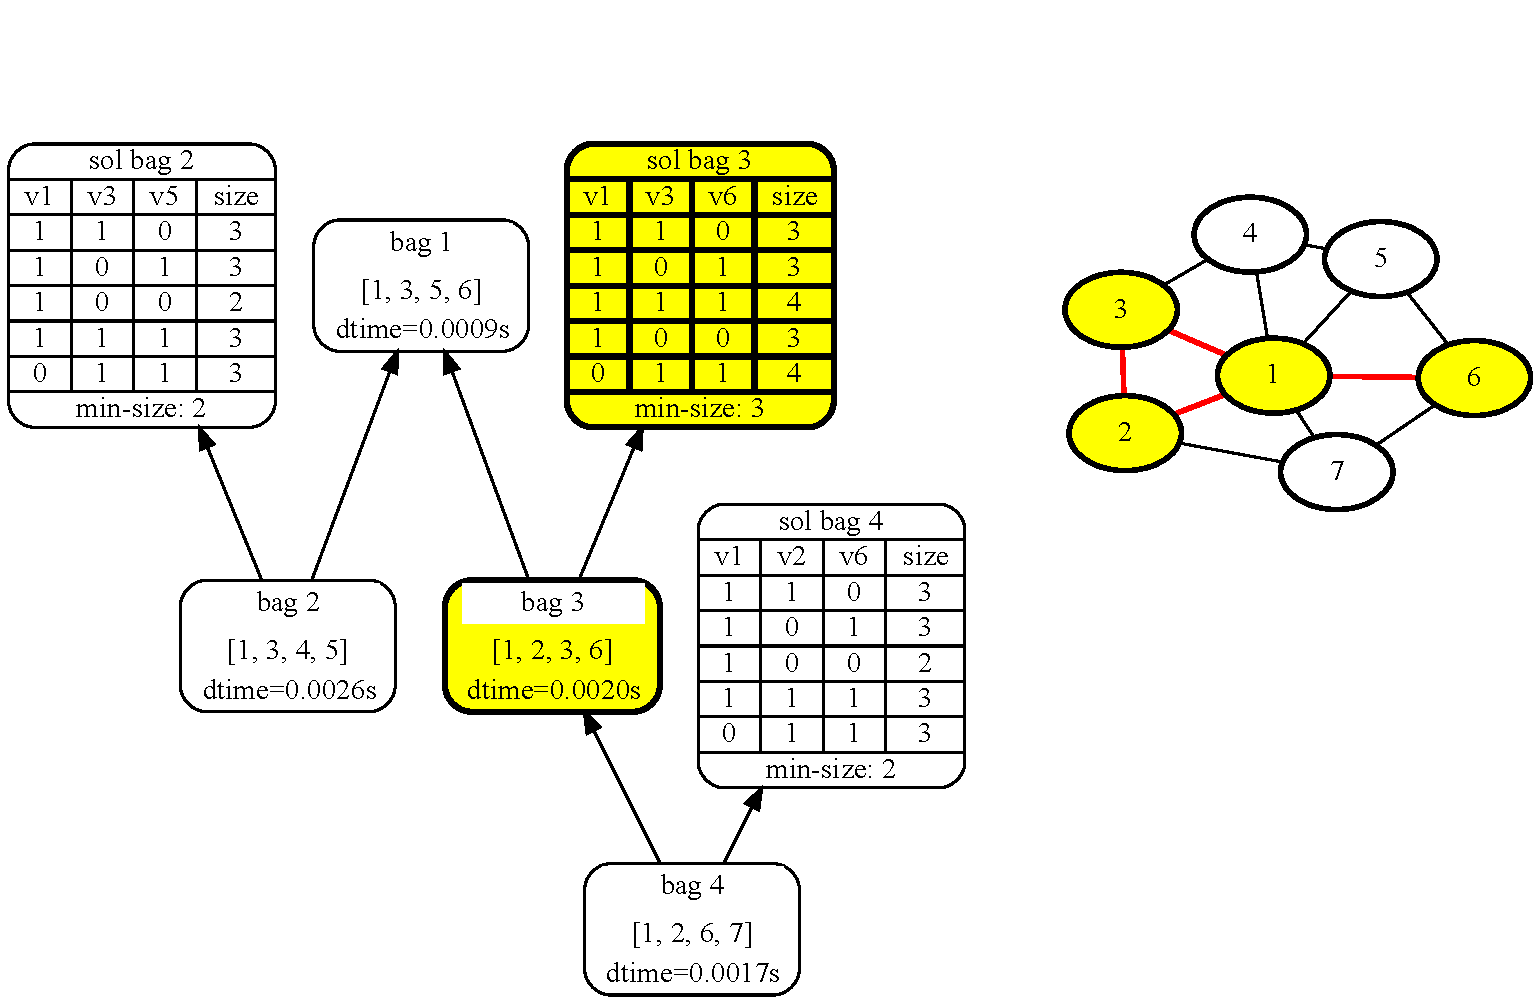
\includegraphics[width=0.99\linewidth]{images/WheelGraph7/combined4.pdf} \\
		\hline 	\\		
		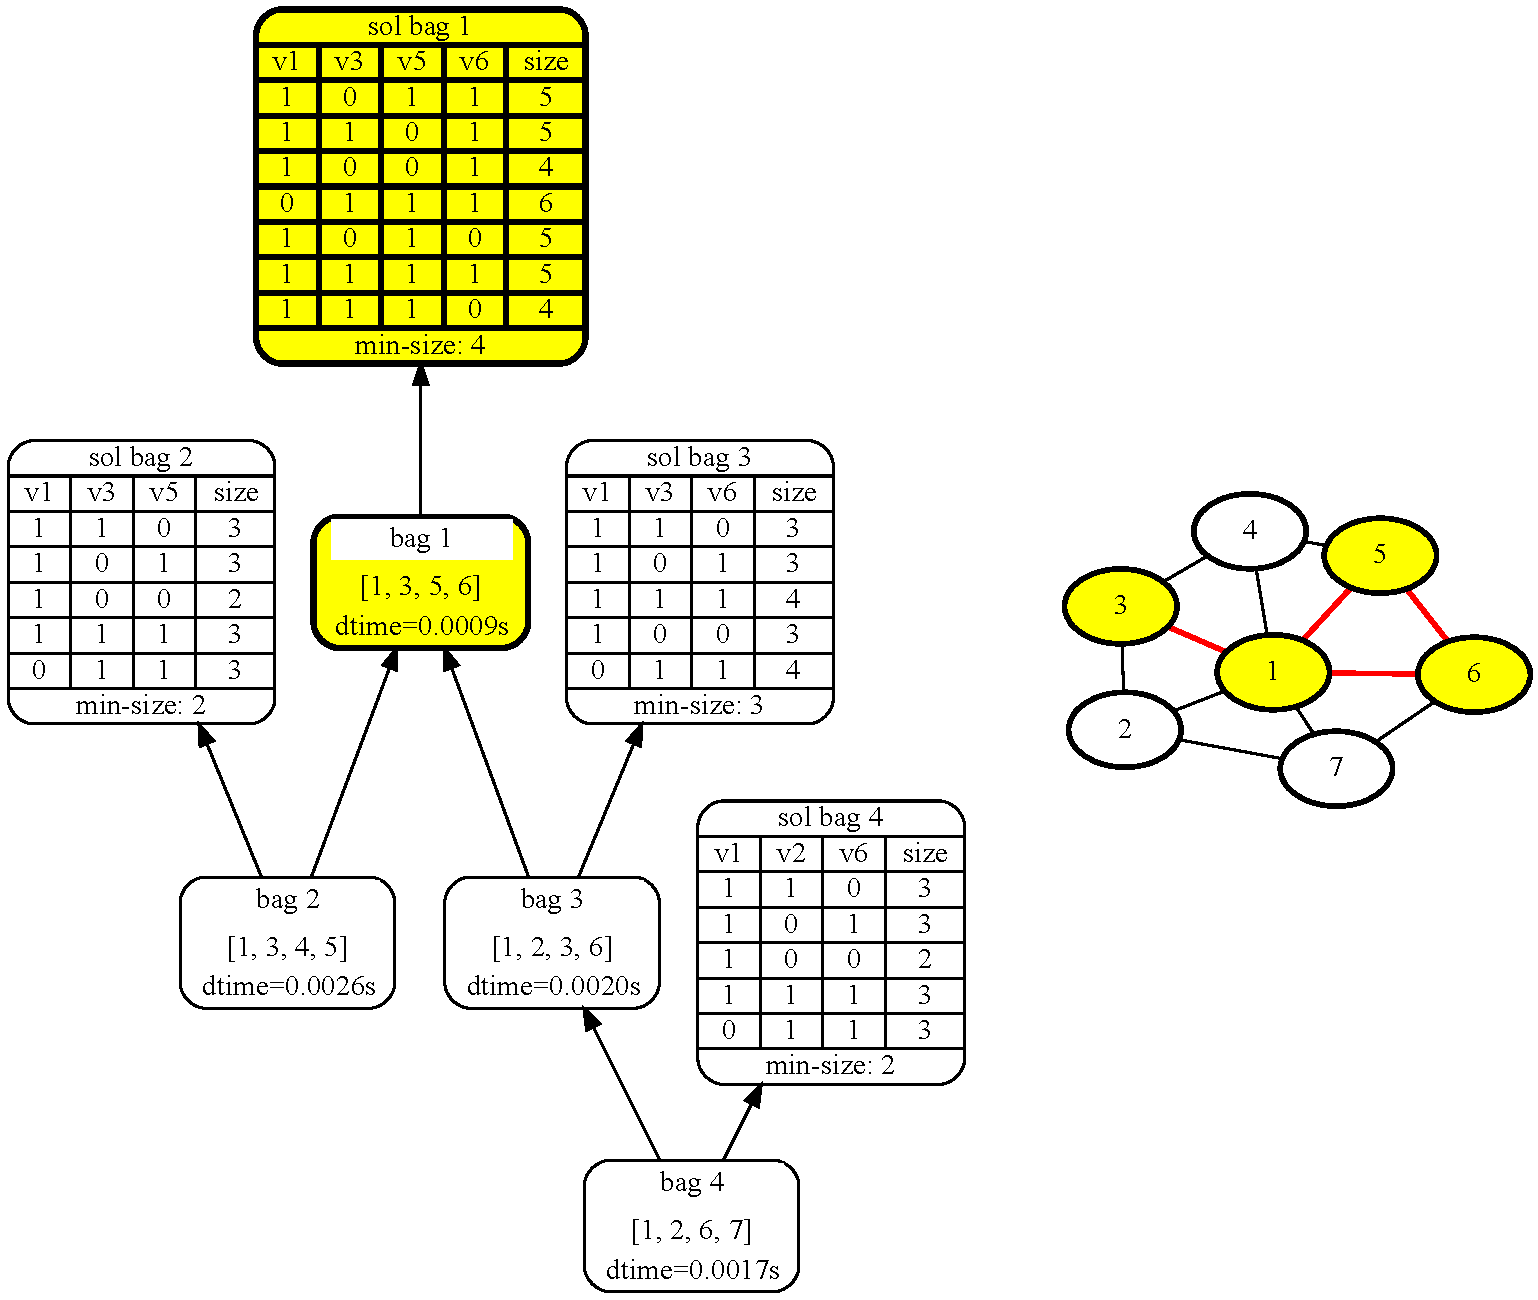
\includegraphics[width=0.95\linewidth]{images/WheelGraph7/combined5.pdf}
	\end{tabular}
	
	\caption[Last steps to solve \textit{minimal vertex cover} for example graph \ref{fig:wheelgraph}]{Last steps, solving \textbf{bag 3} (upper image) and \textbf{bag 1} (lower image), to answer \textit{minimal vertex cover} for our example graph in Fig. \ref{fig:wheelgraph}.}
	\label{fig:wheelgraphc45}
\end{figure}


% Appl. svgjoin with different options
\subsection{SVG Join Example}

After creating several images at each visualization step all images from this step can be automatically combined into one SVG. In this chapter we expand on Section \ref{sec:svgjoin} with some practical applications of this concept.

With the four parameters \textit{padding}, \textit{v\_bottom}, \textit{v\_top} and \textit{scale2} we can specify the order in which images will be placed next to each other. To explain some configurations we will take the generated images from the previous chapter.\\
\noindent
We will first look at some constructed examples using rectangles in the Figures \ref{fig:svgjoinpad0}-\ref{fig:svgjoinscaledbottom}. Then we see some actual applications in Figures~\ref{fig:joindefault}-\ref{fig:join60} at page~\pageref{fig:joindefault}.\noindent\\

\medskip\noindent
Possibilities for joining images with these four parameters include joining with:
\begin{itemize}[label=-, left=40pt]
	\item default \textit{padding}, Fig. \ref{fig:svgjoinpad0}.
	\item \textit{padding} set to 200, Fig. \ref{fig:svgjoinpad200}.
	\item scaling both images to the same size, Fig. \ref{fig:svgjoinscale1}.
	\item aligning both images for vertical centering, Fig. \ref{fig:svgjoinpad0centered}.
	\item uniformly scaling the second image, Fig. \ref{fig:svgjoinscaled}.
	\item scaling and aligning at the bottom edge of the image, Fig. \ref{fig:svgjoinscaledbottom}.
\end{itemize}

\begin{figure}[H]
	\centering
	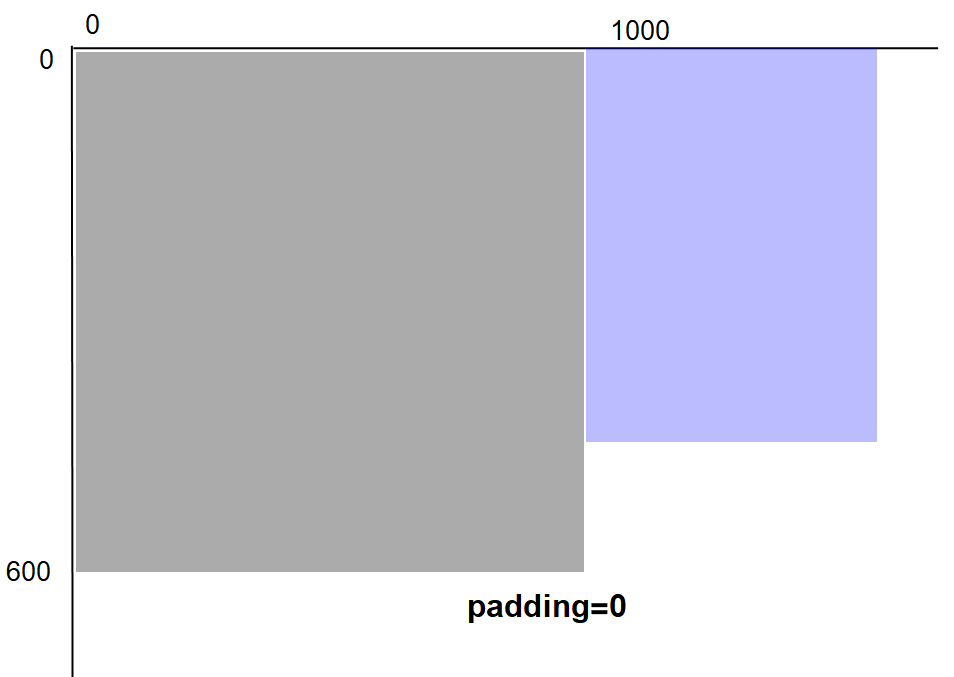
\includegraphics[width=0.6\linewidth]{images/svgjoinpad0nn.png}
	\caption{Example for joining with no \textit{padding}.}
	\label{fig:svgjoinpad0}
\end{figure}

\begin{figure}[H]
	\centering
	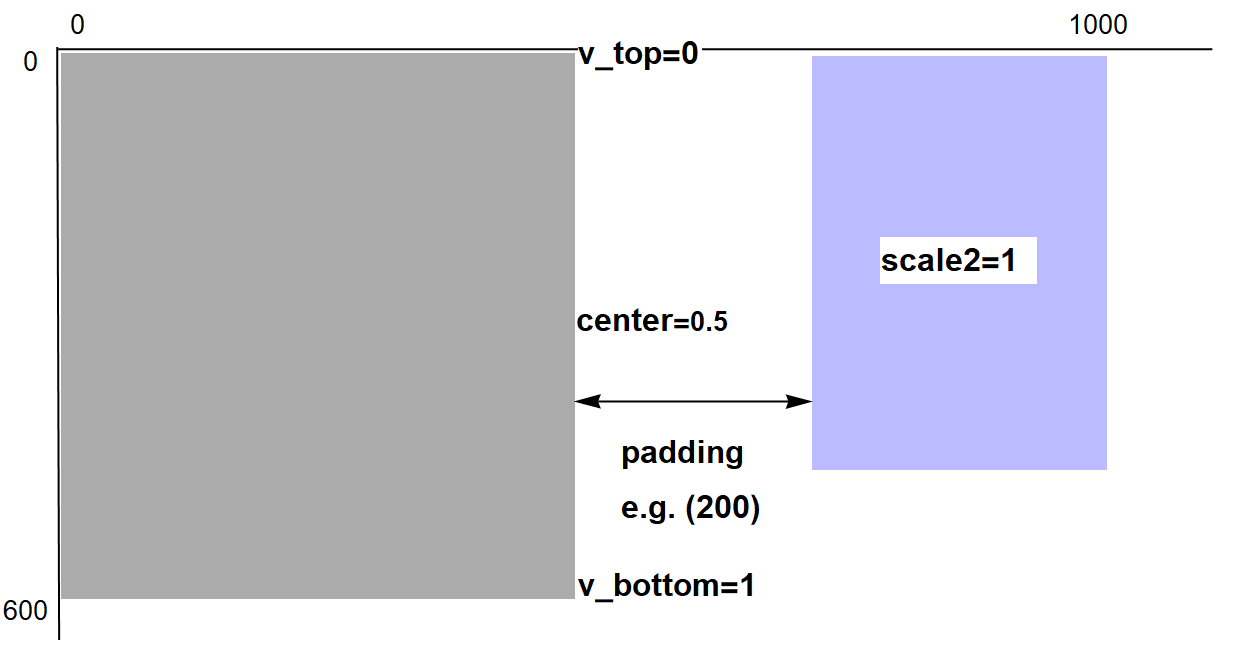
\includegraphics[width=0.8\linewidth]{images/svgjoinpad200nn.png}
	\caption[Joining with padding]{Joining the blue (right side) image to the left gray image with only one parameter \textit{padding} set to 200. We see the default vertical position v\_top=0, and the implied coordinate system with an origin in the top left corner.}
	\label{fig:svgjoinpad200}
\end{figure}

\begin{figure}[H]
	\centering
	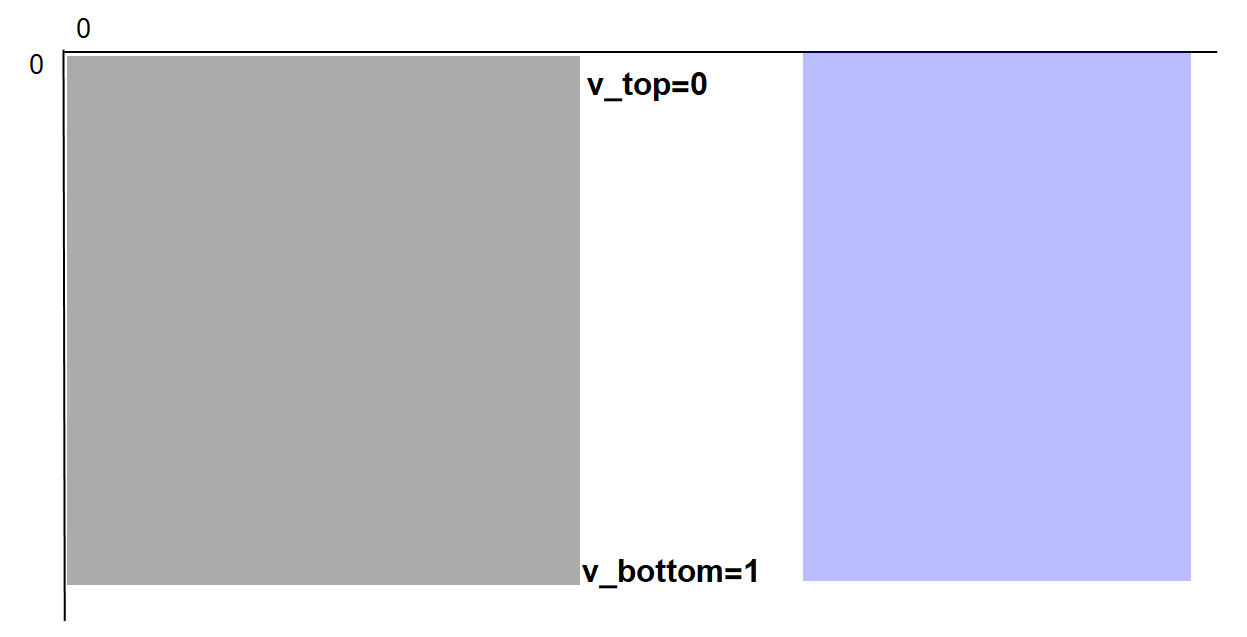
\includegraphics[width=0.8\linewidth]{images/svgjoinscale1nn.png}
	\caption[Joining with same size]{The second image is scaled to the same height as the first image. This can be conveniently achieved by setting \textit{v\_top} to 0 and \textit{v\_bottom} to 1. Parameter \textit{padding} is 200 as hinted.}
	\label{fig:svgjoinscale1}
\end{figure}

\begin{figure}[H]
	\centering
	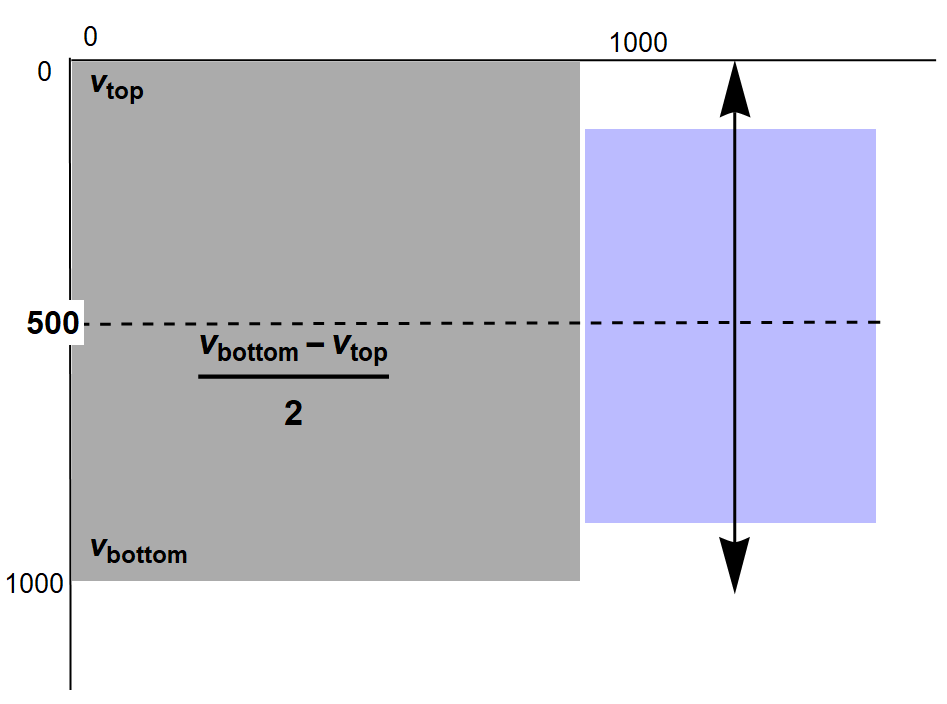
\includegraphics[width=0.8\linewidth]{images/svgjoinpad0centeredn.png}
	\caption[Align both images for vertical centering]{Align both images for vertical centering. \\
		This can be achieved by setting $v\_bottom=v\_top=0.5$.}
	\label{fig:svgjoinpad0centered}
\end{figure}

\begin{figure}[H]
	\centering
	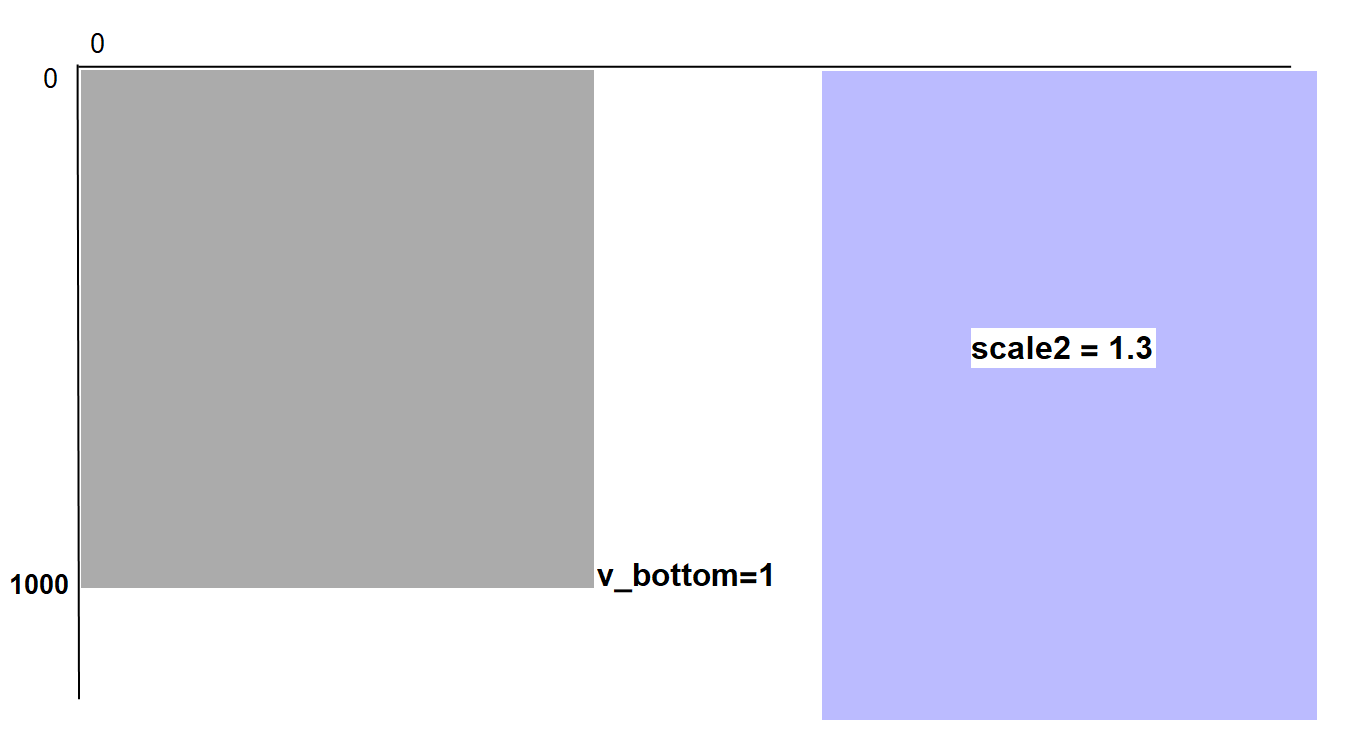
\includegraphics[width=0.8\linewidth]{images/svgjoinscalednn.png}
	\caption[Joining with scaling of $1.3$]{Setting \textit{scale2} to $1.3$ to scale the blue (right) image uniformly. Parameter \textit{padding} is 200 as hinted.}
	\label{fig:svgjoinscaled}
\end{figure}

\begin{figure}[H]
	\centering
	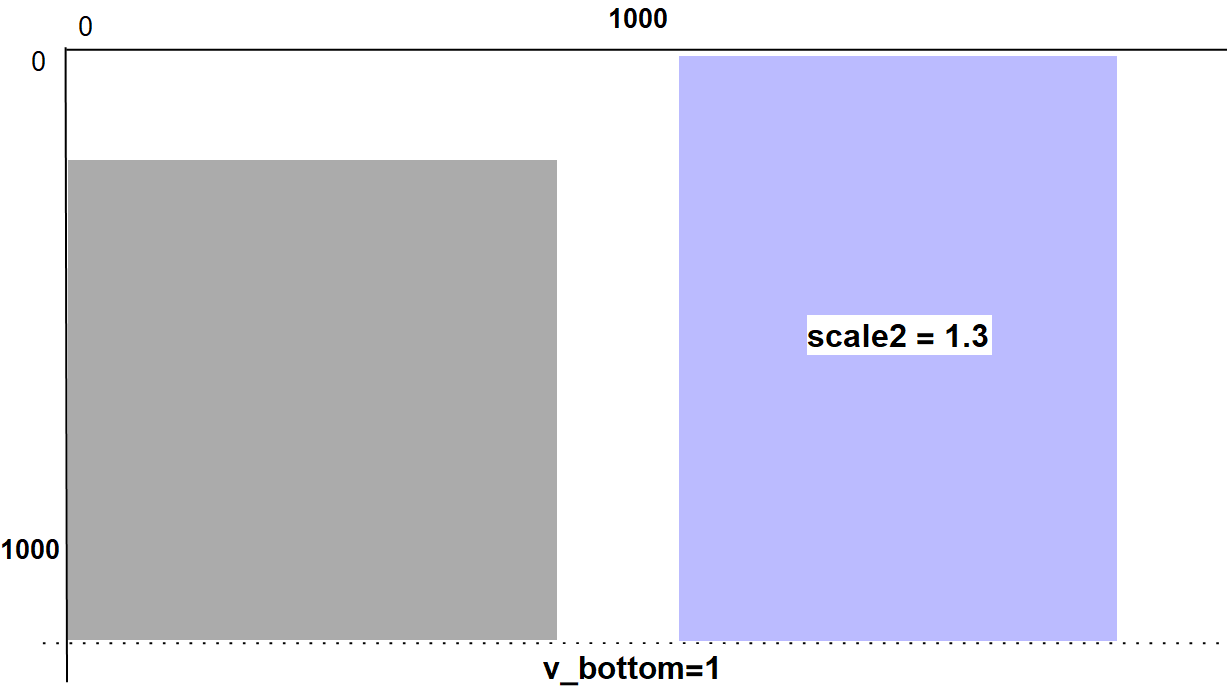
\includegraphics[width=0.8\linewidth]{images/svgjoinscaledbottomnn.png}
	\caption[Joining a scaled image aligned at the bottom edge]{As in figure \ref{fig:svgjoinscaled} we use \textit{scale2} to scale the blue rectangle. To align both images at the bottom edge, we use the value $v\_bottom=1$.}
	\label{fig:svgjoinscaledbottom}
\end{figure}

Now for the applied examples we see in Figure \ref{fig:joindefault} the two images are joined with default values for all parameters, in order (\textit{TDStep, graph}). 

As we can see the solutions for bags other than 2 are hidden in the output but are taken into account in the image size. The right graph is aligned to the upper edge of the left image. With no padding between the images \textit{graph} image is attached to the right edge of the first image visualizing the {tree decomposition}.

\begin{figure}[H]
	\centering
	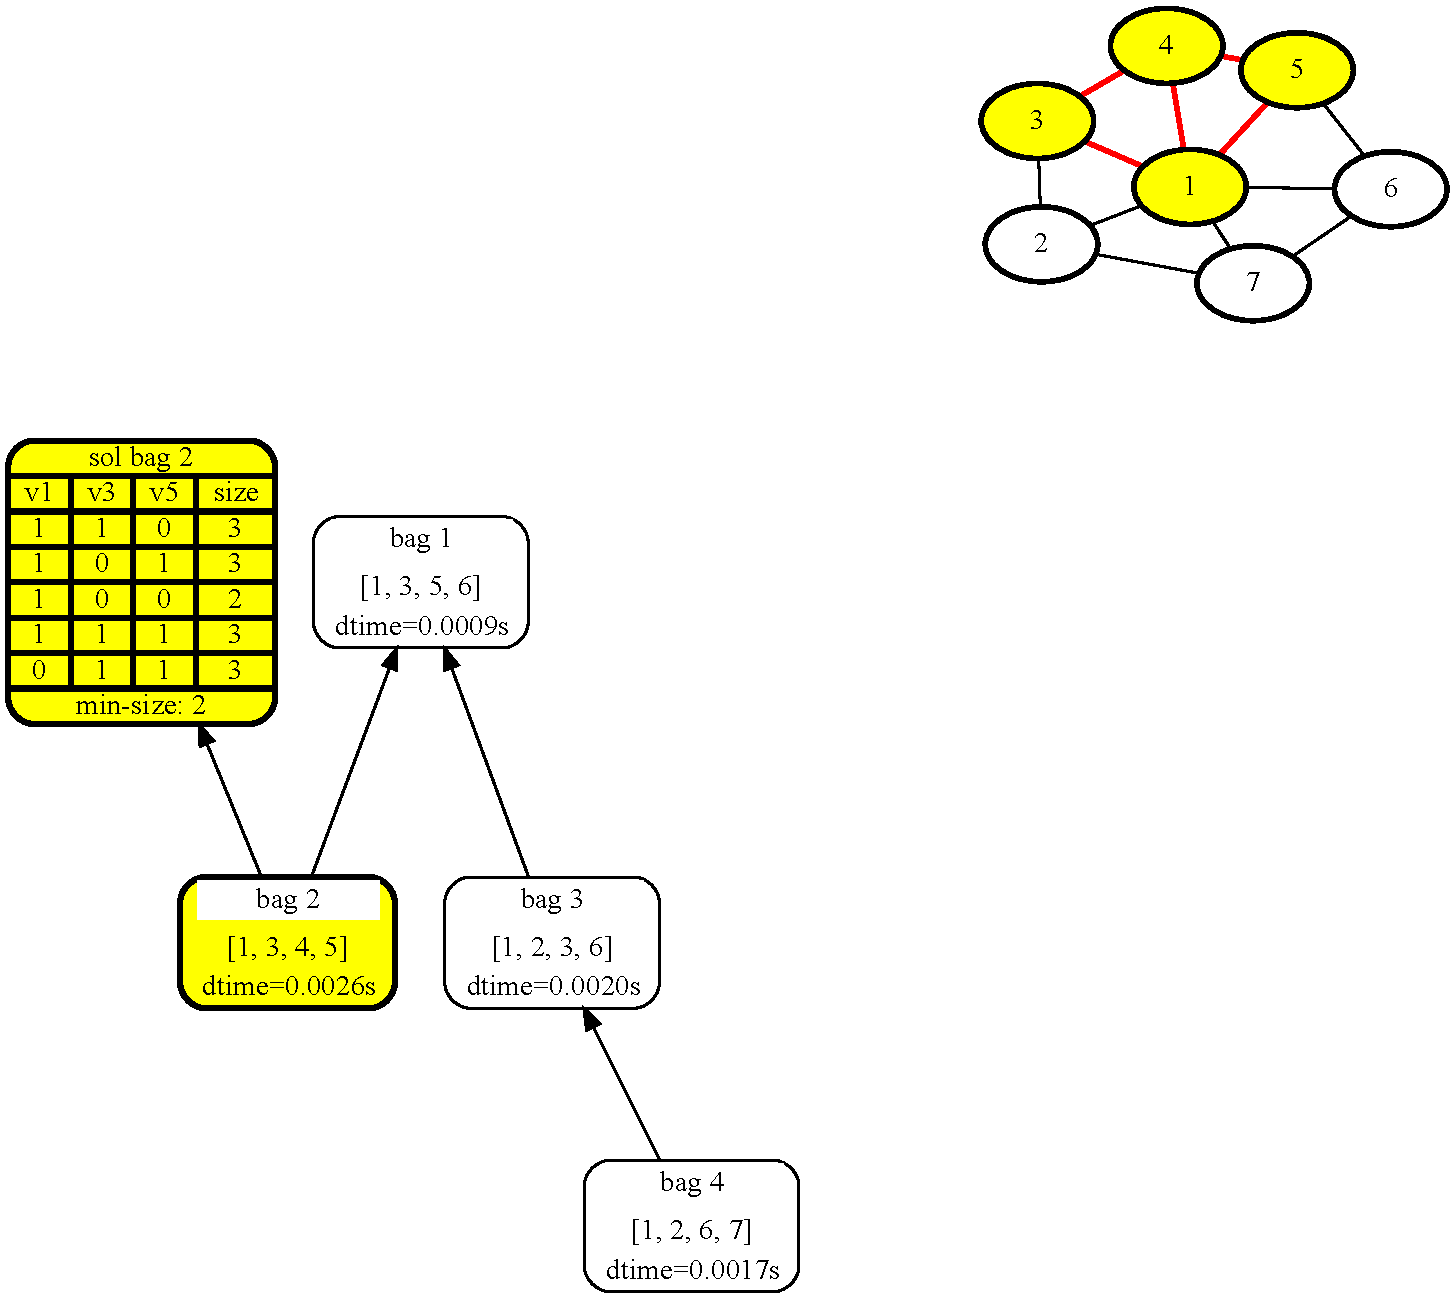
\includegraphics[width=\linewidth,height=0.6\textheight,keepaspectratio]{images/SVGJOIN/default2.pdf}
	\caption[Joining results from Section \ref{sec:minvc} with default parameters at step two]{Joining results from Section \ref{sec:minvc} with default parameters at step two.}
	\label{fig:joindefault}
\end{figure}
%svg_join(['TDStep', 'graph'],
%'Archive/WheelGraph7',
%outname="default_06",
%padding=[0,0,0,40],
%v_bottom=0.6,
%num_images=5)
\begin{figure}[H]
	\centering 
	
	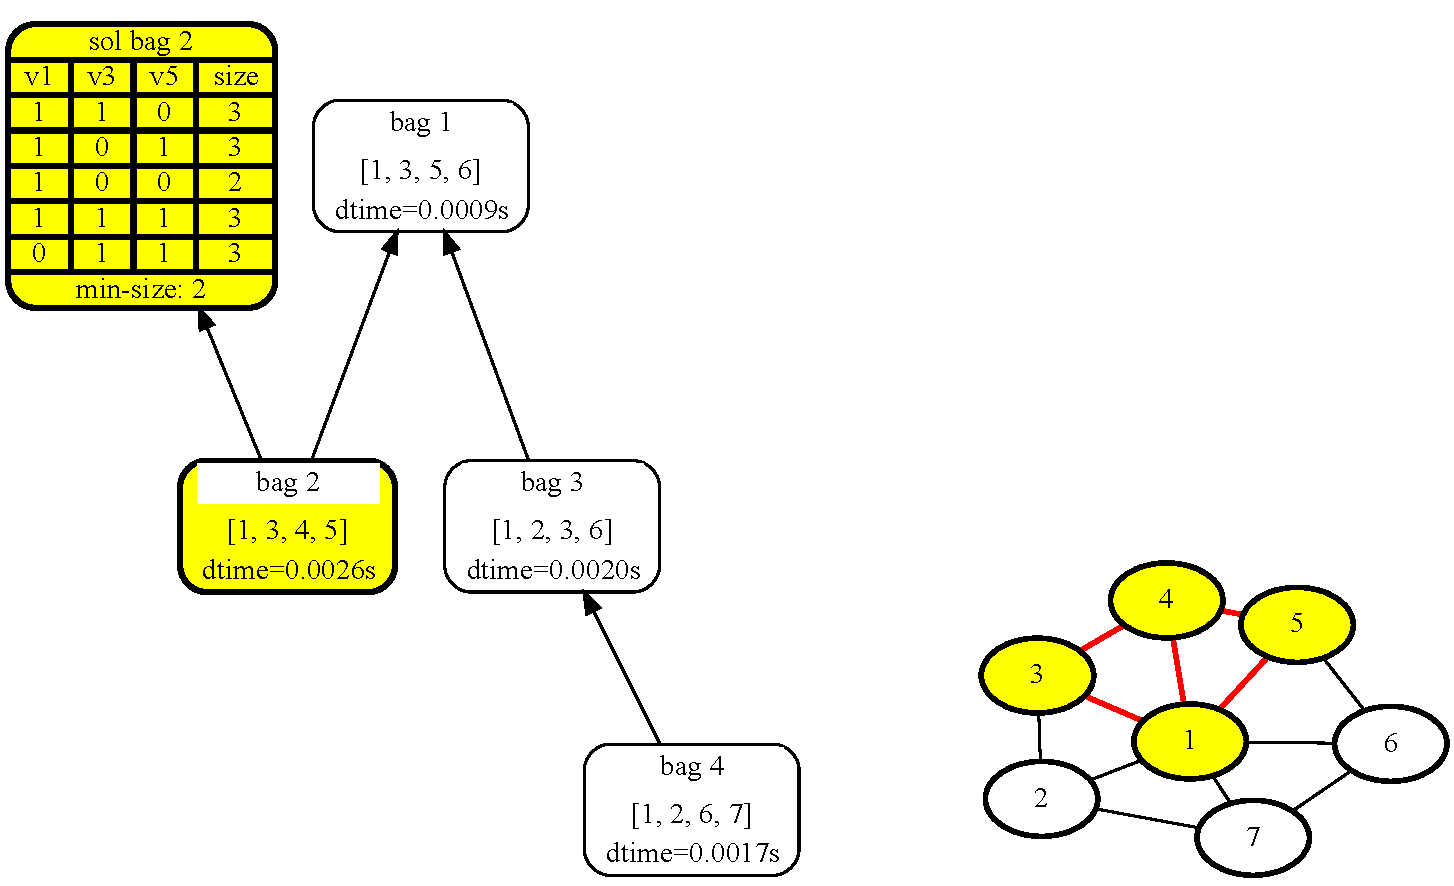
\includegraphics[width=\linewidth]{images/SVGJOIN/default_bottom2.pdf}\\[1.5ex]
	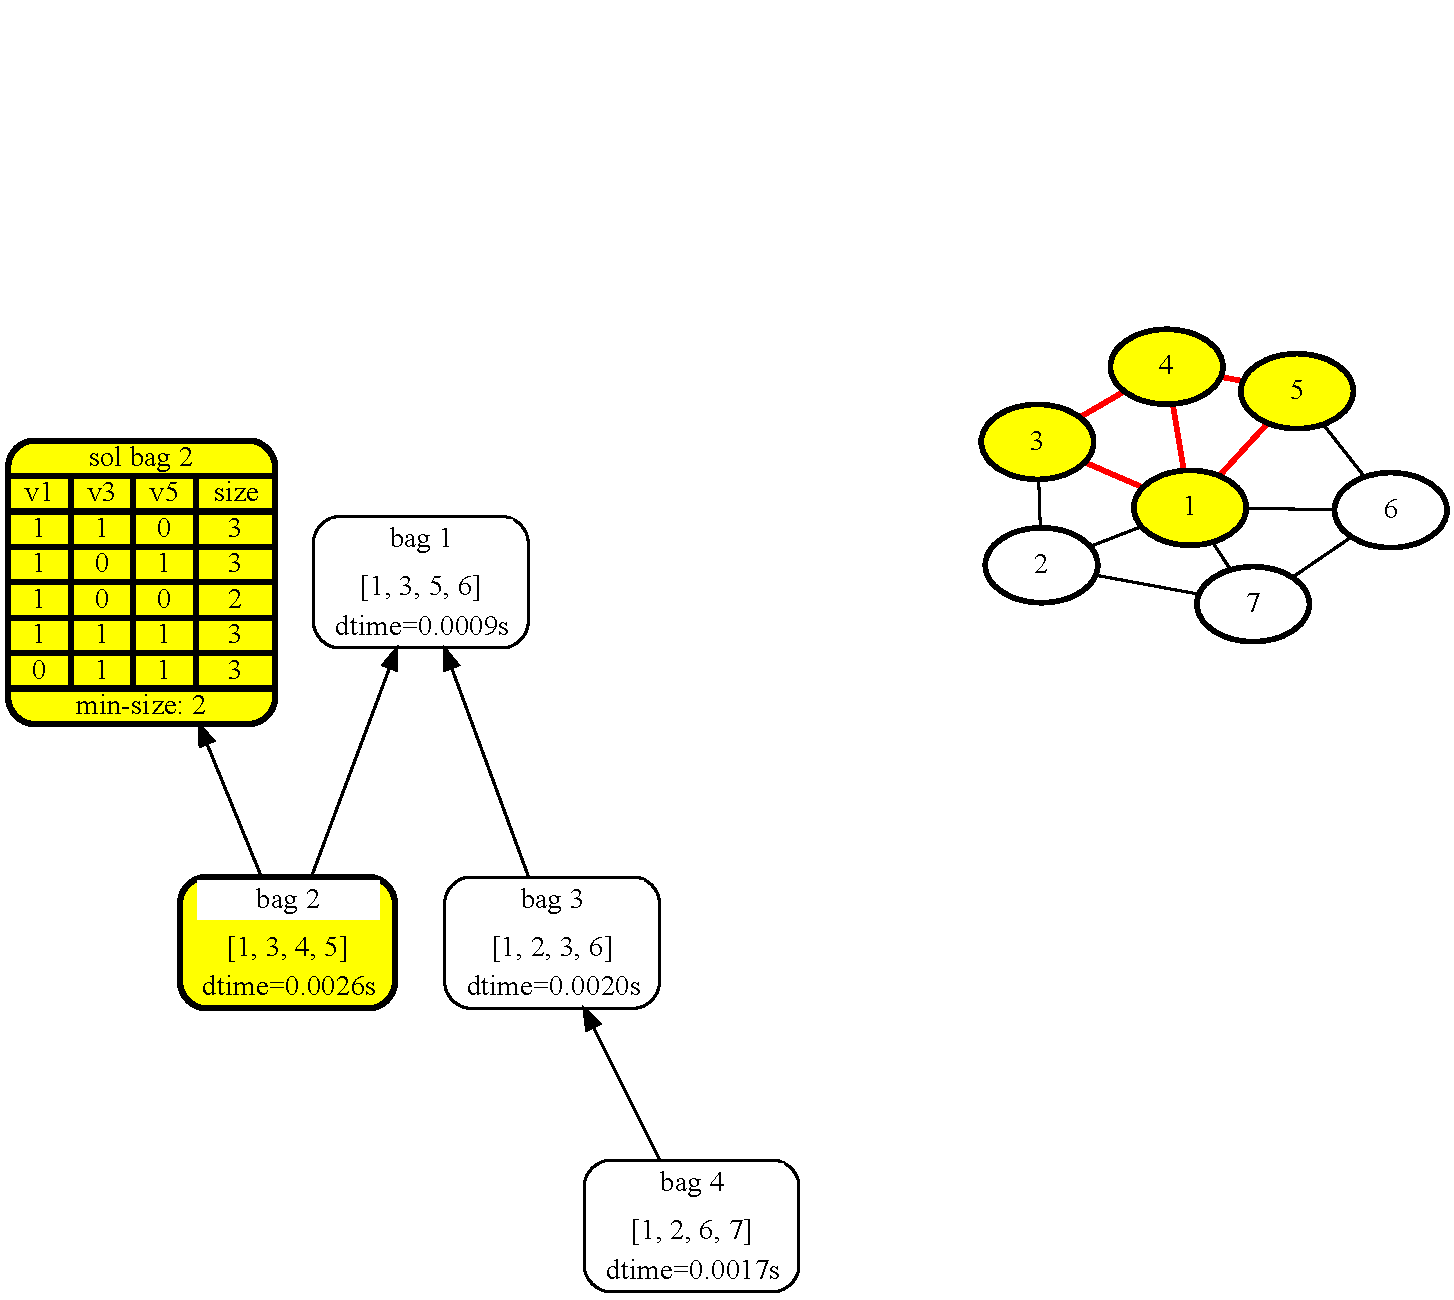
\includegraphics[width=\linewidth]{images/SVGJOIN/default_center2.pdf}
	\caption[Joining results and shifting vertically to bottom and center]{Joining results from Section \ref{sec:minvc} at step two and setting \textit{v\_bottom} to either ``bottom" (upper picture) or ``center" (lower picture). The invisible (empty) parts of the graphics is cropped from the top of each.}
	\label{fig:joinbotcenter}
\end{figure}
\begin{figure}[H]
	\centering
	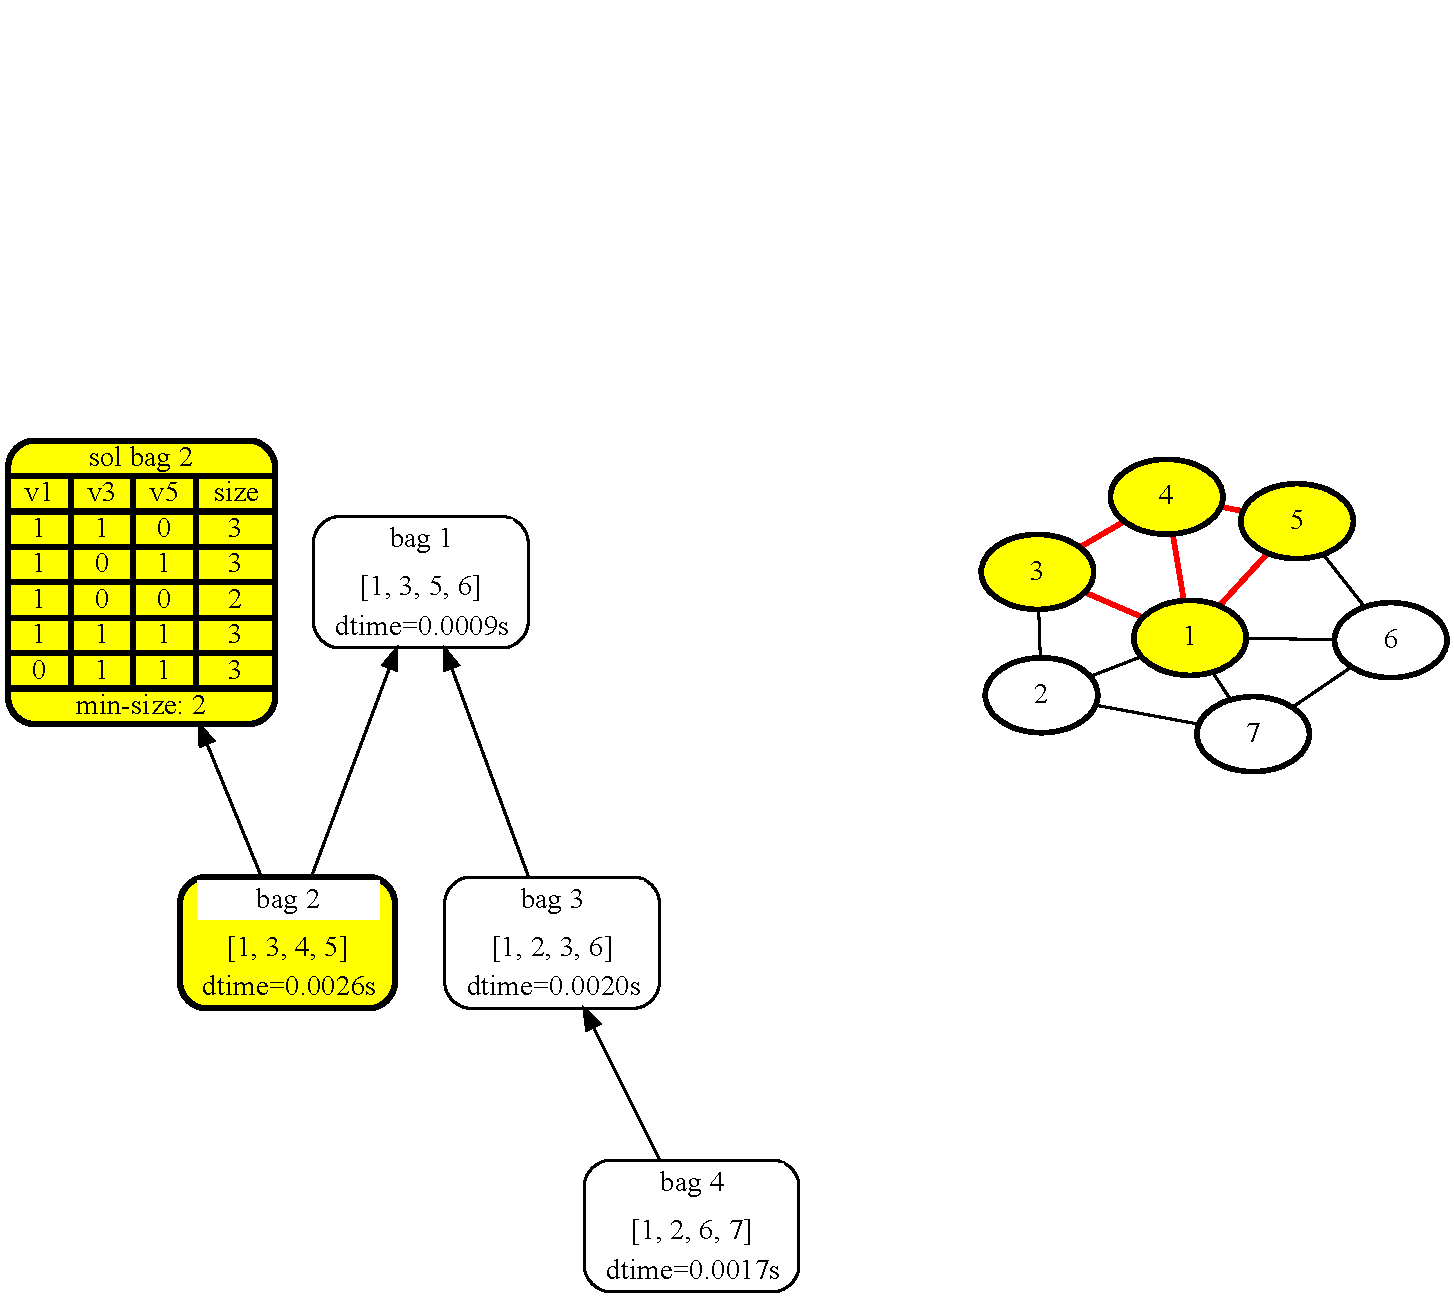
\includegraphics[width=0.9\linewidth,height=0.9\textheight,keepaspectratio]{images/SVGJOIN/default_062.pdf}
	\caption[Joining results and shifting vertically to 60\%]{Joining results from Section \ref{sec:minvc} at step two and shifting bottom edge of second image to $60\%$ height of the first image.}
	\label{fig:join60}
\end{figure}

In Figure \ref{fig:joinbotcenter} the parameter v\_bottom is set to ``bottom" to align both graphics on the bottom edge; set to ``center" elevates the right image to 50\% of the height of the first. It is also possible to provide arbitraty floating-point values for vertical adjustment as presented in Figure \ref{fig:join60} with \textit{v\_bottom = 0.6}.

If we want the right graph a bit larger compared to the default size, we can add additional scaling by providing the argument \textbf{scale2}. In figures \ref{fig:joinscaled1} to \ref{fig:joinscaled5} the complete time series for solving \textit{minimal vertex cover} for example \ref{lst:wheelgraph} with join-parameters
\begin{itemize}
	\item[] padding = [ 0, 0, 0, 40 ],\quad v\_bottom = 0.6,\quad scale2 = 1.5
\end{itemize}
can be seen. \\
To further visualize the progress of the algorithm in the results one could use the option to specify multiple values for all the transformation parameters and for example elevate the second image with the values for
\begin{itemize}
\item[] v\_bottom = [ 1, 0.85, 0.7, 0.55, 0.4 ]
\end{itemize}
 This is done in figures \ref{fig:joinscaledrise1} to \ref{fig:joinscaledrise5} on page~\pageref{fig:joinscaledrise1}.

% Finding a bug using visualization
\subsection{Visualization of Defects}
 
As stated in the introduction, most of the data we visualize is already present in the solvers.
Given the right testing frameworks it is possible to produce a report for structural or even randomly occurring defects in the solver. As the software we used for our experimental visualizations shown in this work does not itself contain a test environment, we were able to produce some undiscovered ``bugs" while using and developing our visualization tool.


 One specific program invocation did not give the expected result solving a \textit{vertex cover} with one hundred nodes. The problem was first found when inspecting the immediate output of the program \textit{dpdb.py}, which did report the wrong result size. The problem could be localized in the tree decomposition, leading to the whole result table being pruned - see the visualization in Figure \ref{fig:starsbag59}. It is obvious that ``bag 59" is disconnected from its parent ``bag 57", even if its nodes occurred in other bags in the tree. This violates our rule $3$ of the TD (``the set of bags that contain the variable v induce a connected sub-graph of T.").  This particular bug only occurred  with a specific seed (zero) and on the Windows operating system (not on the tested Linux systems). 

\begin{figure}
	\centering
	\vspace{1em}
	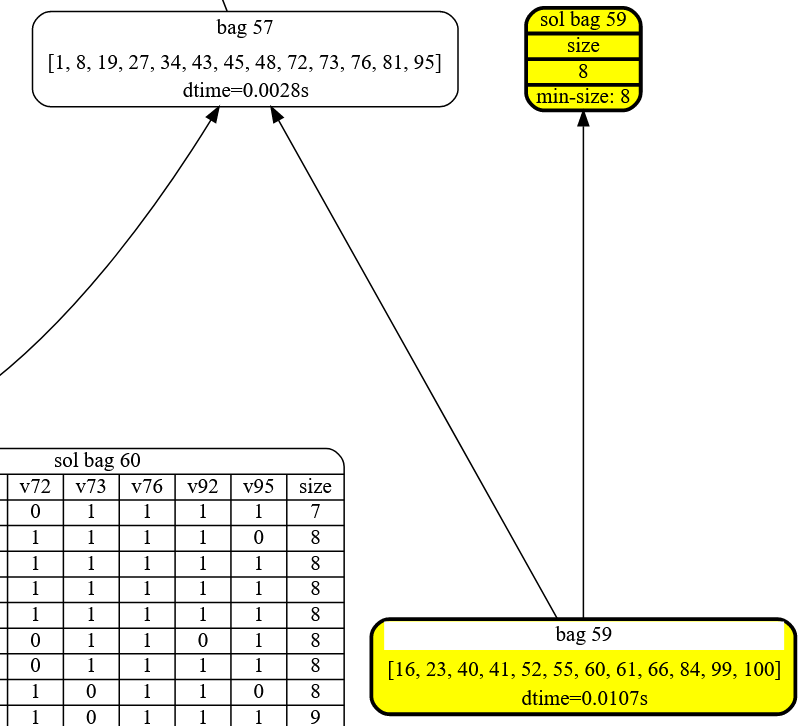
\includegraphics[width=0.8\linewidth,height=0.9\textheight,keepaspectratio
					]{images/starsbag59.png}
		\vspace{1em}
	\caption[Section of interest to find the problem with bag 59 visualized]{Section of interest to find the problem with bag 59 visualized.}
	\label{fig:starsbag59}
\end{figure}

%\begin{figure}[H]
%	\centering
%	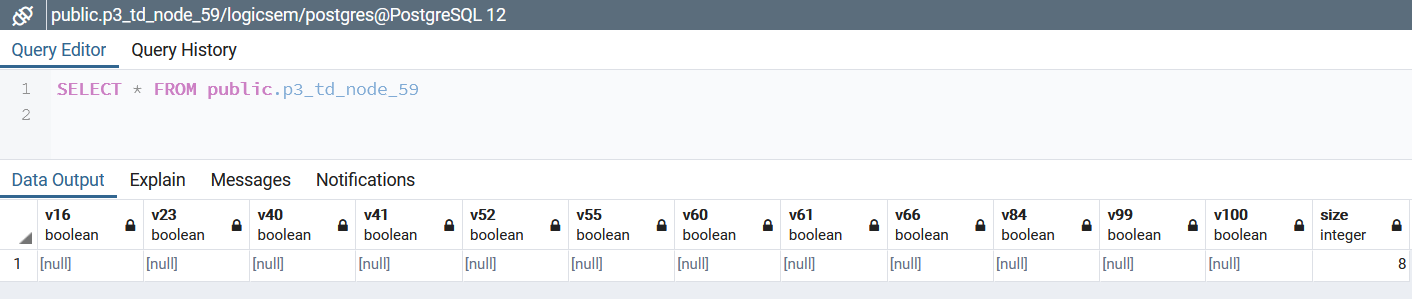
\includegraphics[width=0.9\linewidth,height=0.9\textheight,keepaspectratio]{images/Found bag 59 in stars100 with seed0.png}
%	\caption{Bag 59 in the database table.}
%	\label{fig:bag59visu}
%\end{figure}

The problem was located in the version of \url{github.com/TU-Wien-DBAI/htd} used to create the tree decomposition, which in this instance did not place bag 59 in the right place in the tree-decomposition on our Windows 10 machine. We can see the bags of the tree decomposition in Figure \ref{fig:bag59td}, where the bags containing variable $v_{100}$ are indicated in red. 

\begin{figure}
	\centering
	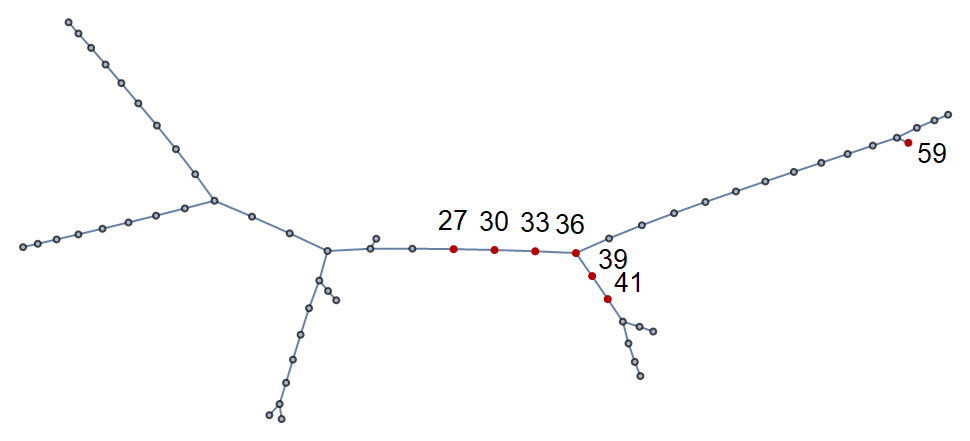
\includegraphics[width=0.9\linewidth,height=0.9\textheight,keepaspectratio]{images/stars100var100.png}
	\caption[Simplified graphic of the TD with bags in red that contain the variable $v_{100}$]{Simplified graphic of the TD with bags in red that contain the variable $v_{100}$. Bag 59 can be seen separated on the far right of the figure.}
	\label{fig:bag59td}
\end{figure}
%==============================================================================
%============== Conclusion ====================================================
%==============================================================================
\section{Conclusion}\label{sec:conclusion}
%What is achieved?
% Open source Assistant for visualizing dynamic programming on tree decompositions
% Small dataformat, highly adaptable svg format
% Two example integrations in actively developed MSO solvers
% Bags do provide the option to add arbitrary many/long labels for different debugging information
\subsection{Summary}
We created a program which can automate the visualization of dynamic programming on tree decompositions. All tree decomposition nodes are prepared to display multiple user-defined strings, which can contain various debugging information about the run.
With SVG we support by default a fast and easily editable image format.\\

The visualization is implemented in two actively developed solvers for the problem types {SAT}, {\#SAT} and {minimal vertex cover}. We have tested the visualization of each problem type with graphs of different sizes - with nodes in the order of $10^{0..2}$ for MinVC and $10^{0..3}$ for SAT and \#SAT.

During the development we could already find some bugs in the solvers.

We have defined a data exchange API to give the visualization the information it needs and provided meaningful default values for most parameters. The API supports the interchange of:
\begin{itemize}
	\item One tree decomposition
	\item Time steps that add solutions to the TD
	\item Incidence graphs for problems on boolean formulas, from which primal and dual graphs can be created automatically
	\item Simple graphs for general graph problems
	\item The merging of several visualizations of a time step into one image
\end{itemize}

\subsection{Future Work}
% Graphs could provide more options to the user
% Generate multiple bipartite and general graphs
% Operate on hypergraphs
% Bring all timesteps into one file, e.g Animations
In the future our graphs could provide even more parameters to the user. \\
Different colors visualizing attributes of each node are a consideration.\\
Show path of various solutions from leaf to bag. \\
The next step would be to expand the API to multiple bipartite or simple graphs, which right now is limited to one each with the option to create primal- and dual-graphs too.\\
One addition would be the inclusion of hypergraphs (graphs where one edge does connect multiple nodes) which could be of great interest for future solvers.\\
Right now even with the \textit{svg-join} tool we need multiple files to represent all time steps. SVG however would be able to only create one file where the time steps will be animated. Animations might get toggled by the user or change over a specified time span.\\

%==============================================================================
%============== APPENDIX ======================================================
%==============================================================================

\appendix
\singlespacing
%============== Images ======================================================
\section{Images}
%\begin{figure}[H]
%	\centering
%	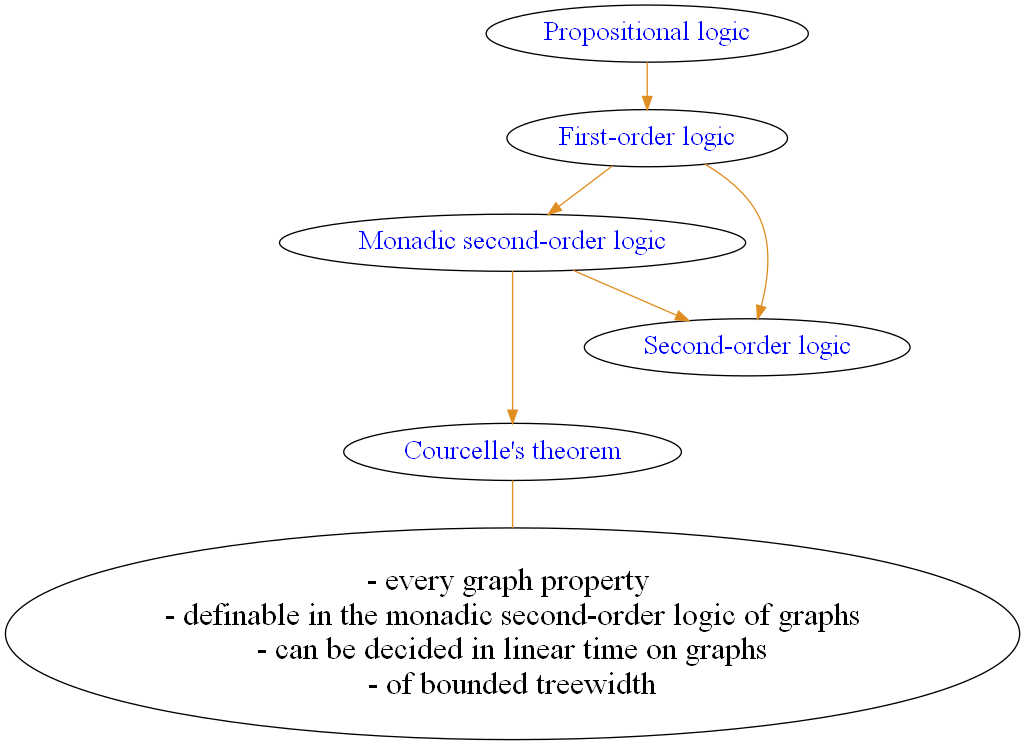
\includegraphics[width=0.8\linewidth]{images/logictheory.png}
%	\caption{From propositional logic to monadic second order logic and Courcelle's Theorem}
%	\label{fig:logictheory}
%\end{figure}
\begin{figure}[H]
	\centering
	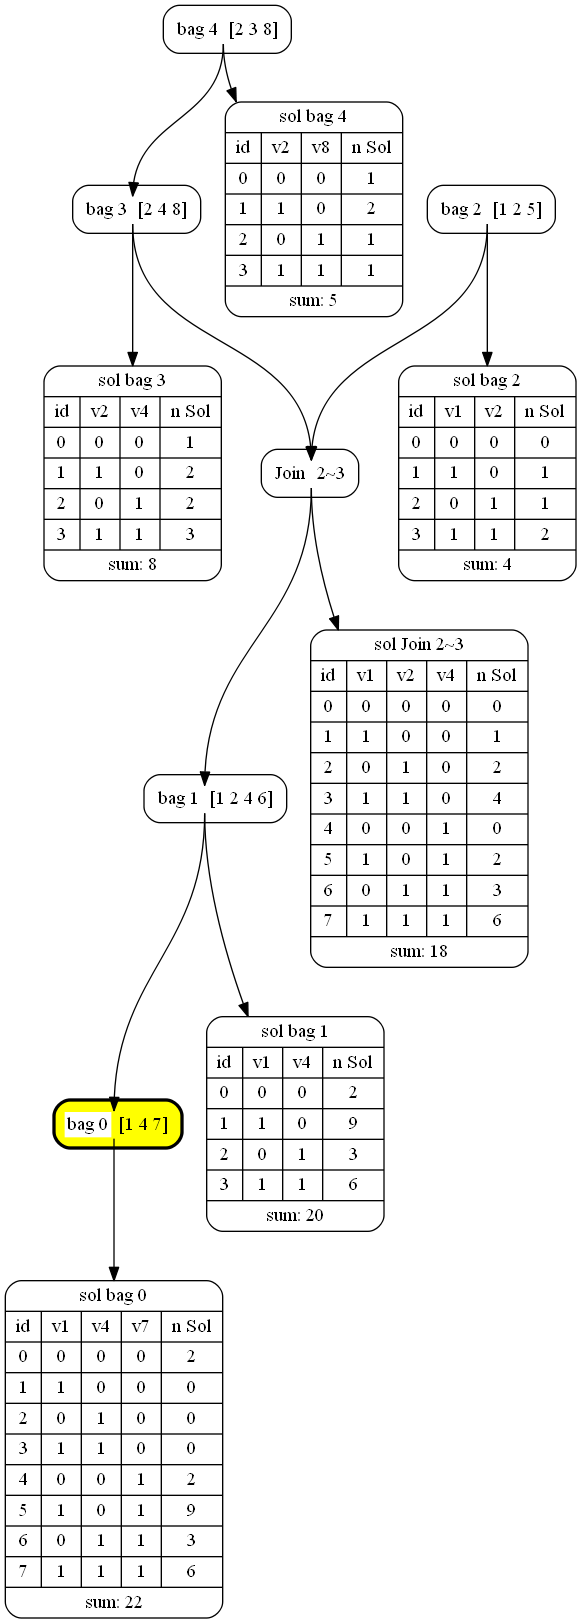
\includegraphics[height=0.93\textheight]{images/g41digraphdot.png}
	\caption{Created scalable-vector-graphic directly from \ref{lst:g41digraphdot}}
	\label{fig:g41Digraph}
\end{figure}

%svg_join(['TDStep', 'graph'],
%'Archive/WheelGraph7',
%outname="default_06sc15",
%padding=[0,0,0,40],
%v_bottom=0.6,
%scale2=1.5,
%num_images=5)


\begin{figure}[H]
	\centering
	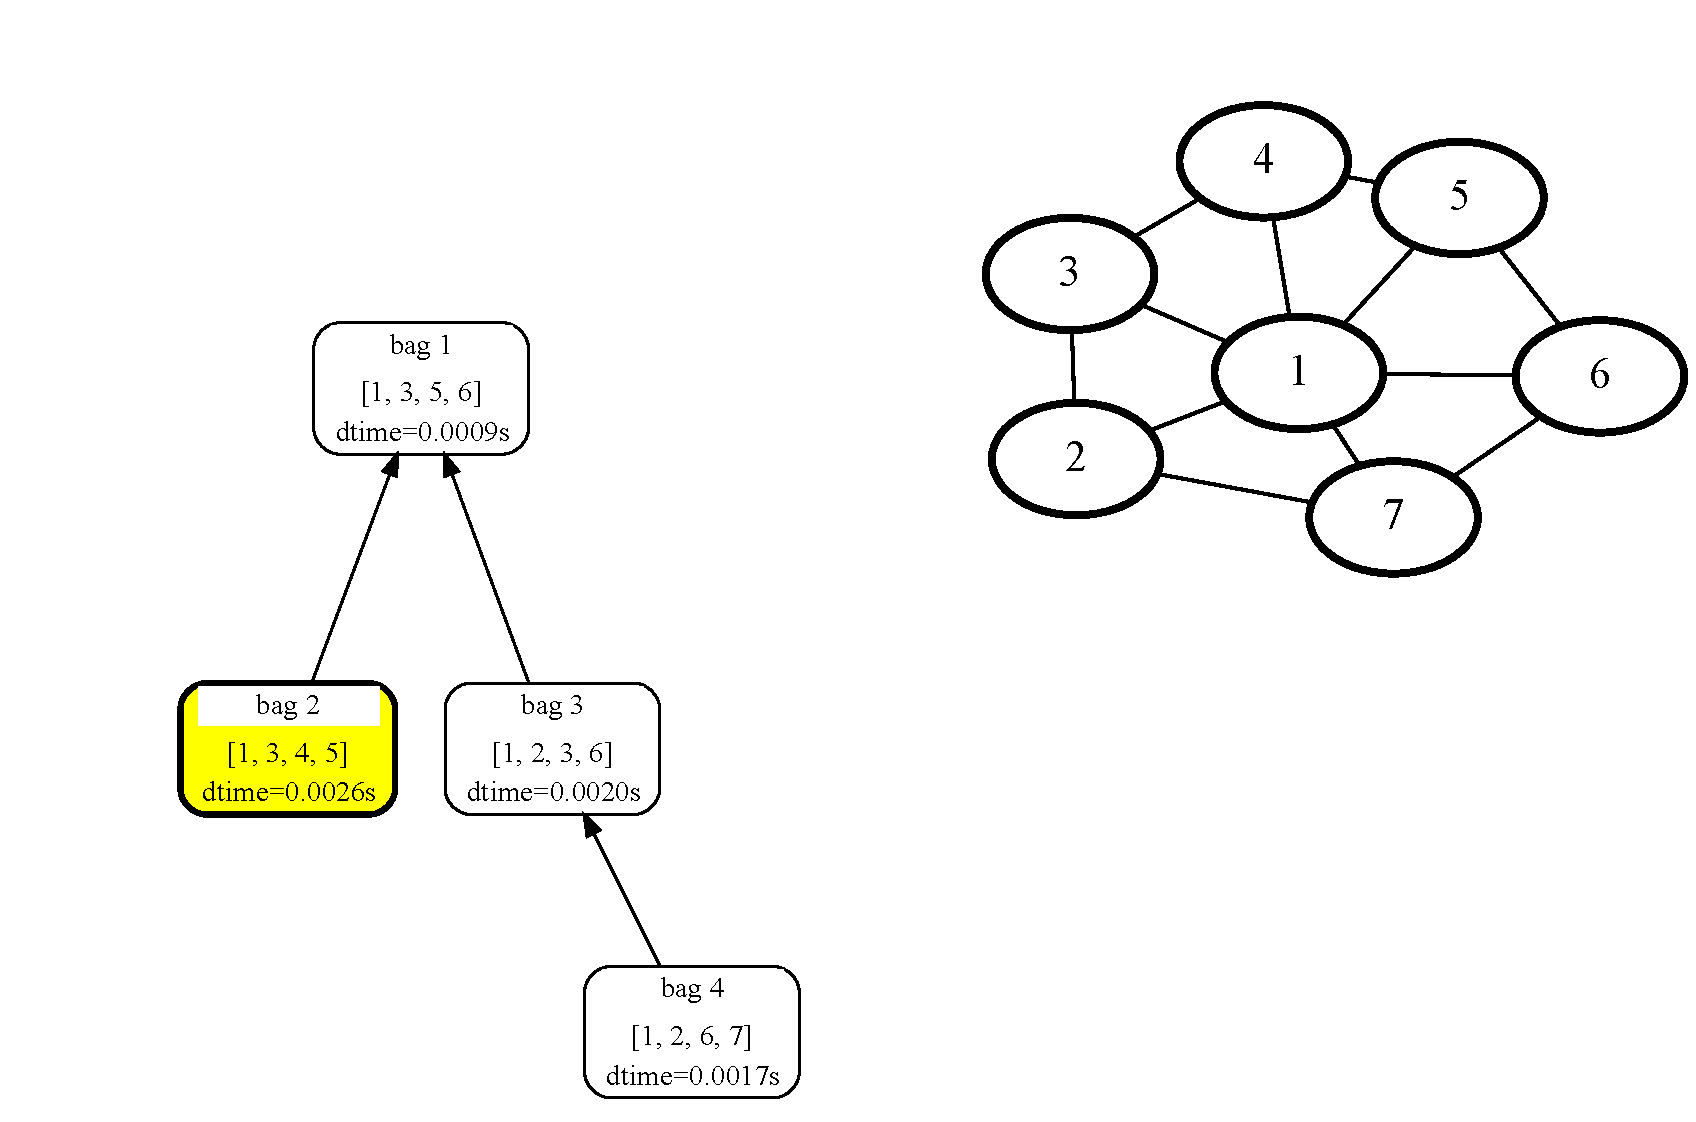
\includegraphics[width=0.9\linewidth,height=0.9\textheight,keepaspectratio]{images/SVGJOIN/default_06sc151.pdf}
	\caption[Joining results from Section \ref{sec:minvc} at step 1/5]{Joining results from Section \ref{sec:minvc} at step 1. Also shifting the second graphic to $40\%$ height of the first image and scaling with scale2 = 1.5 .}
	\label{fig:joinscaled1}
\end{figure}
\begin{figure}[H]
	\centering
	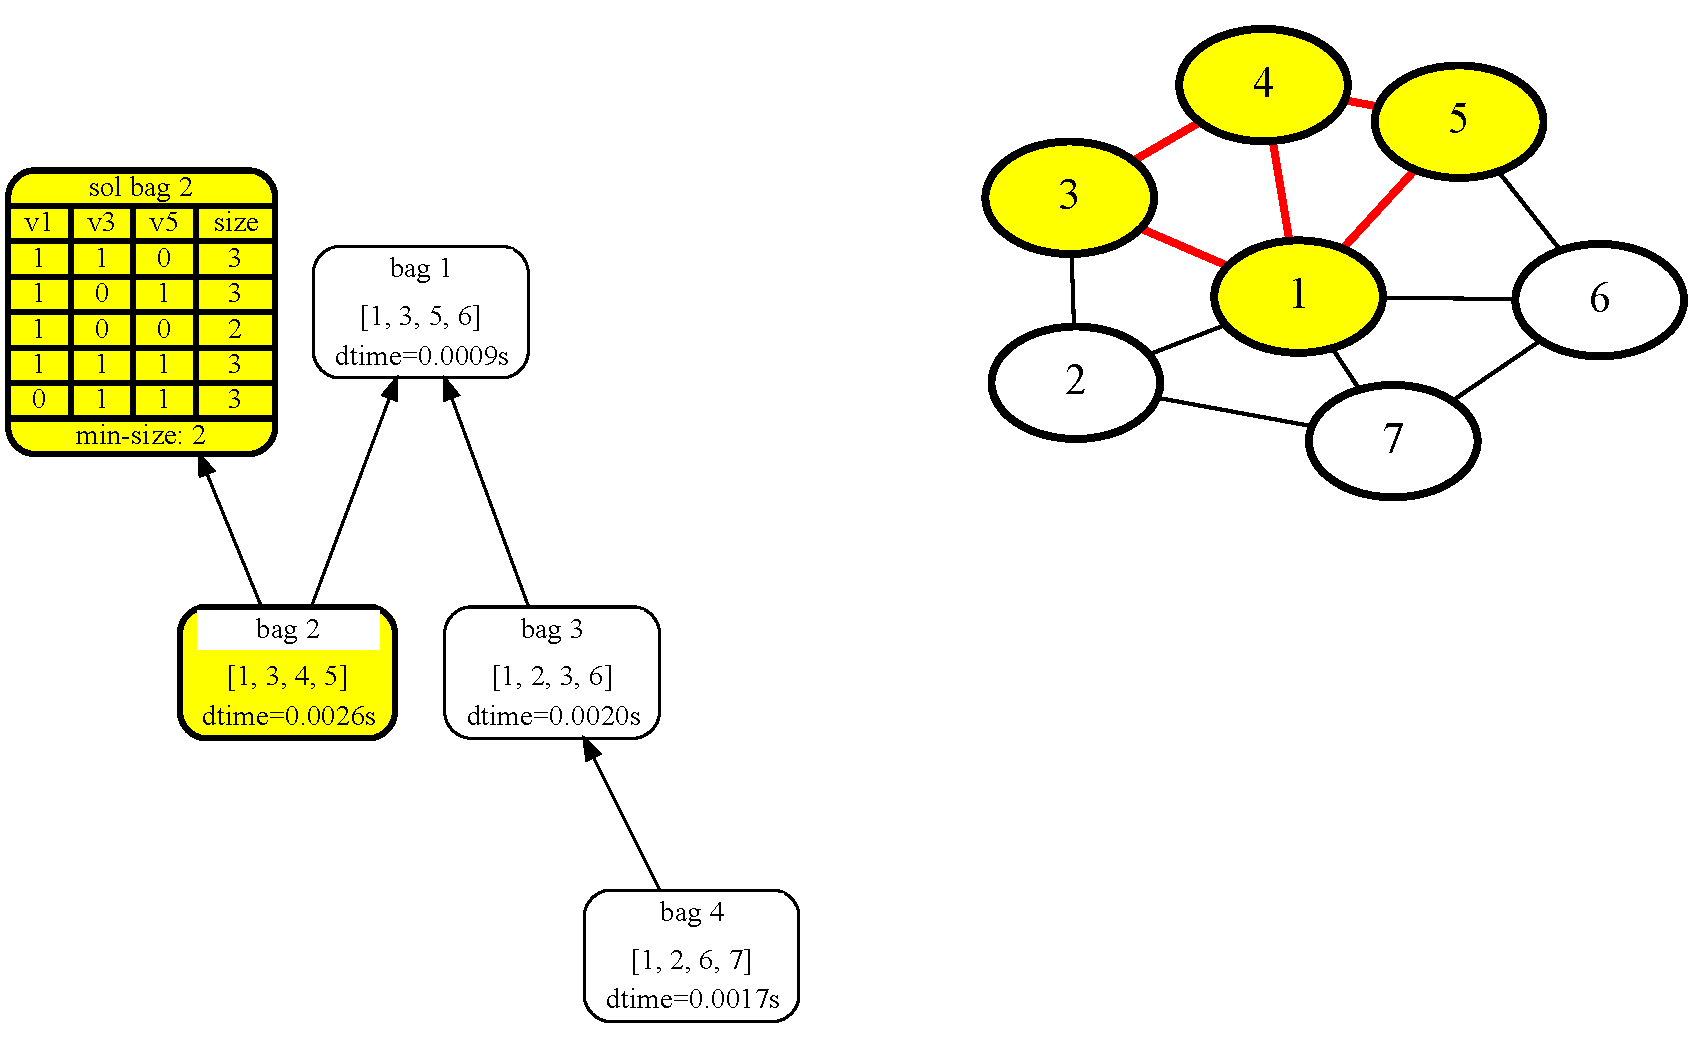
\includegraphics[width=0.9\linewidth,height=0.9\textheight,keepaspectratio]{images/SVGJOIN/default_06sc152.pdf}
	\caption[Joining results from Section \ref{sec:minvc} at step 2/5]{Joining results from Section \ref{sec:minvc} at step two. Also shifting the second graphic to $40\%$ height of the first image and scaling with scale2 = 1.5 .}
	\label{fig:joinscaled2}
\end{figure}
\begin{figure}[H]
	\centering
	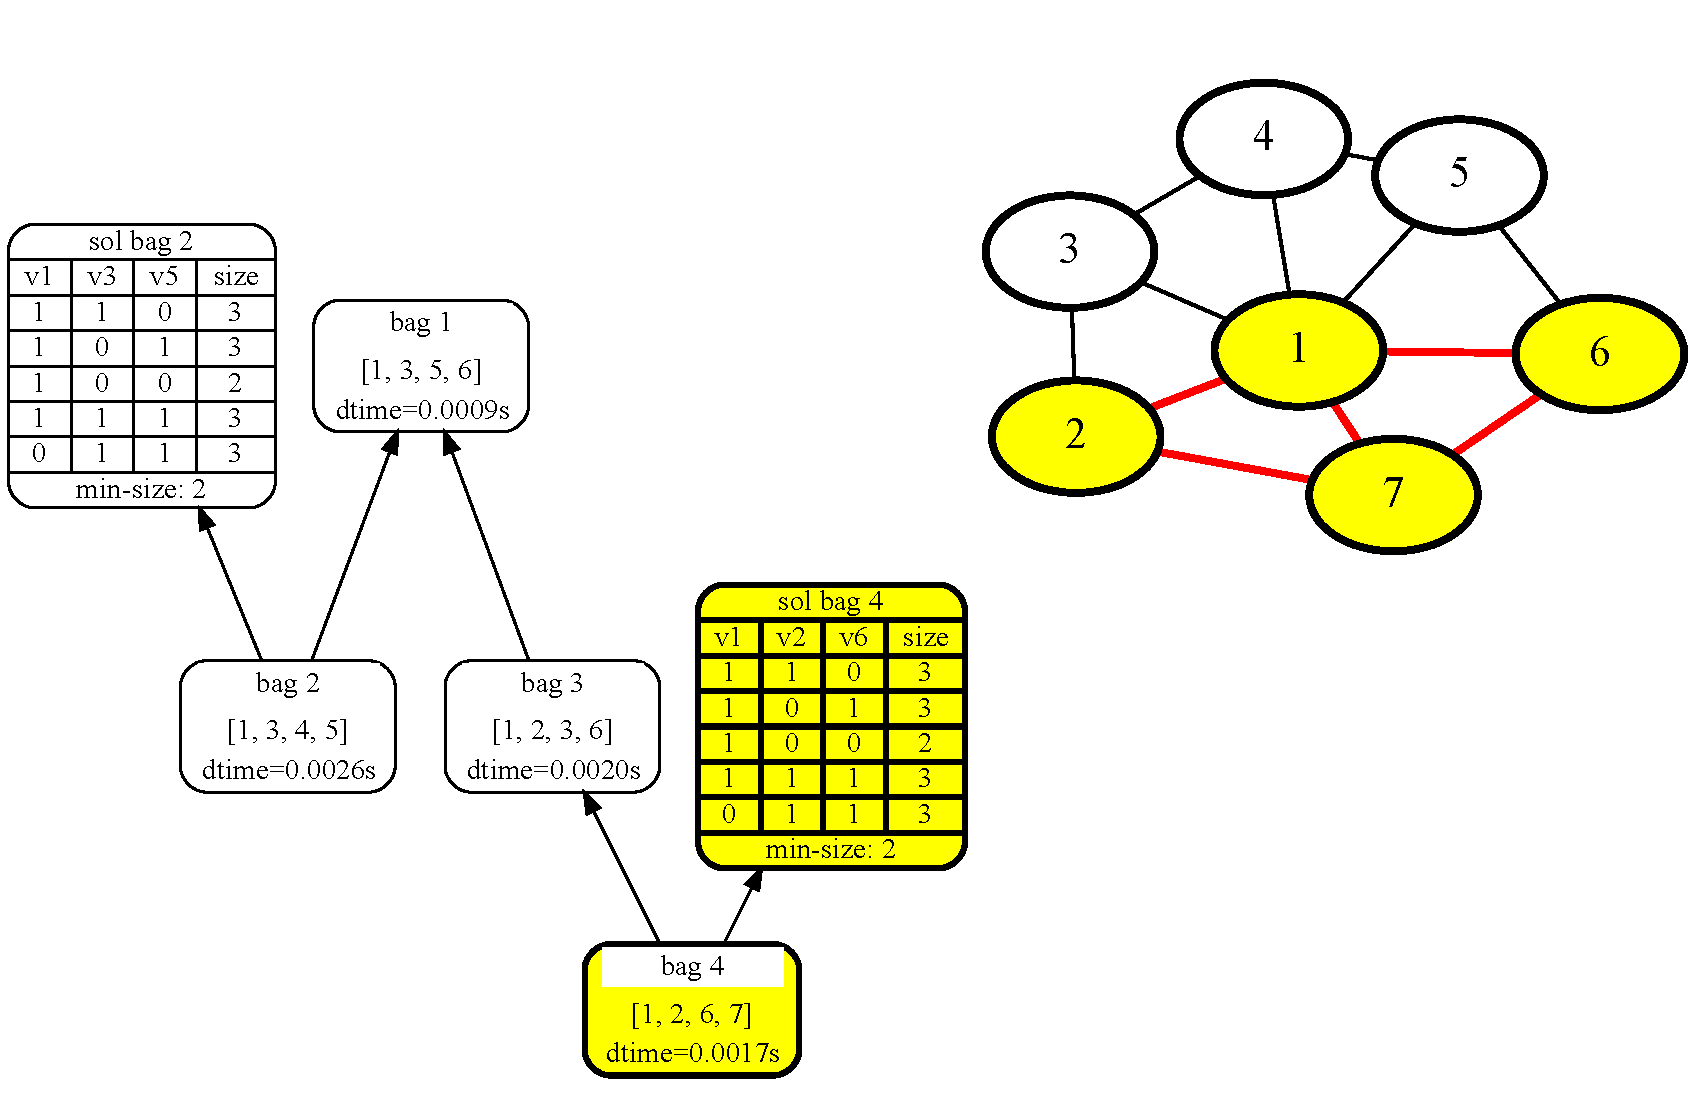
\includegraphics[width=0.9\linewidth,height=0.9\textheight,keepaspectratio]{images/SVGJOIN/default_06sc153.pdf}
	\caption[Joining results from Section \ref{sec:minvc} at step 3/5]{Joining results from Section \ref{sec:minvc} at step 3. Also shifting the second graphic to $40\%$ height of the first image and scaling with scale2 = 1.5 .}
	\label{fig:joinscaled3}
\end{figure}
\begin{figure}[H]
	\centering
	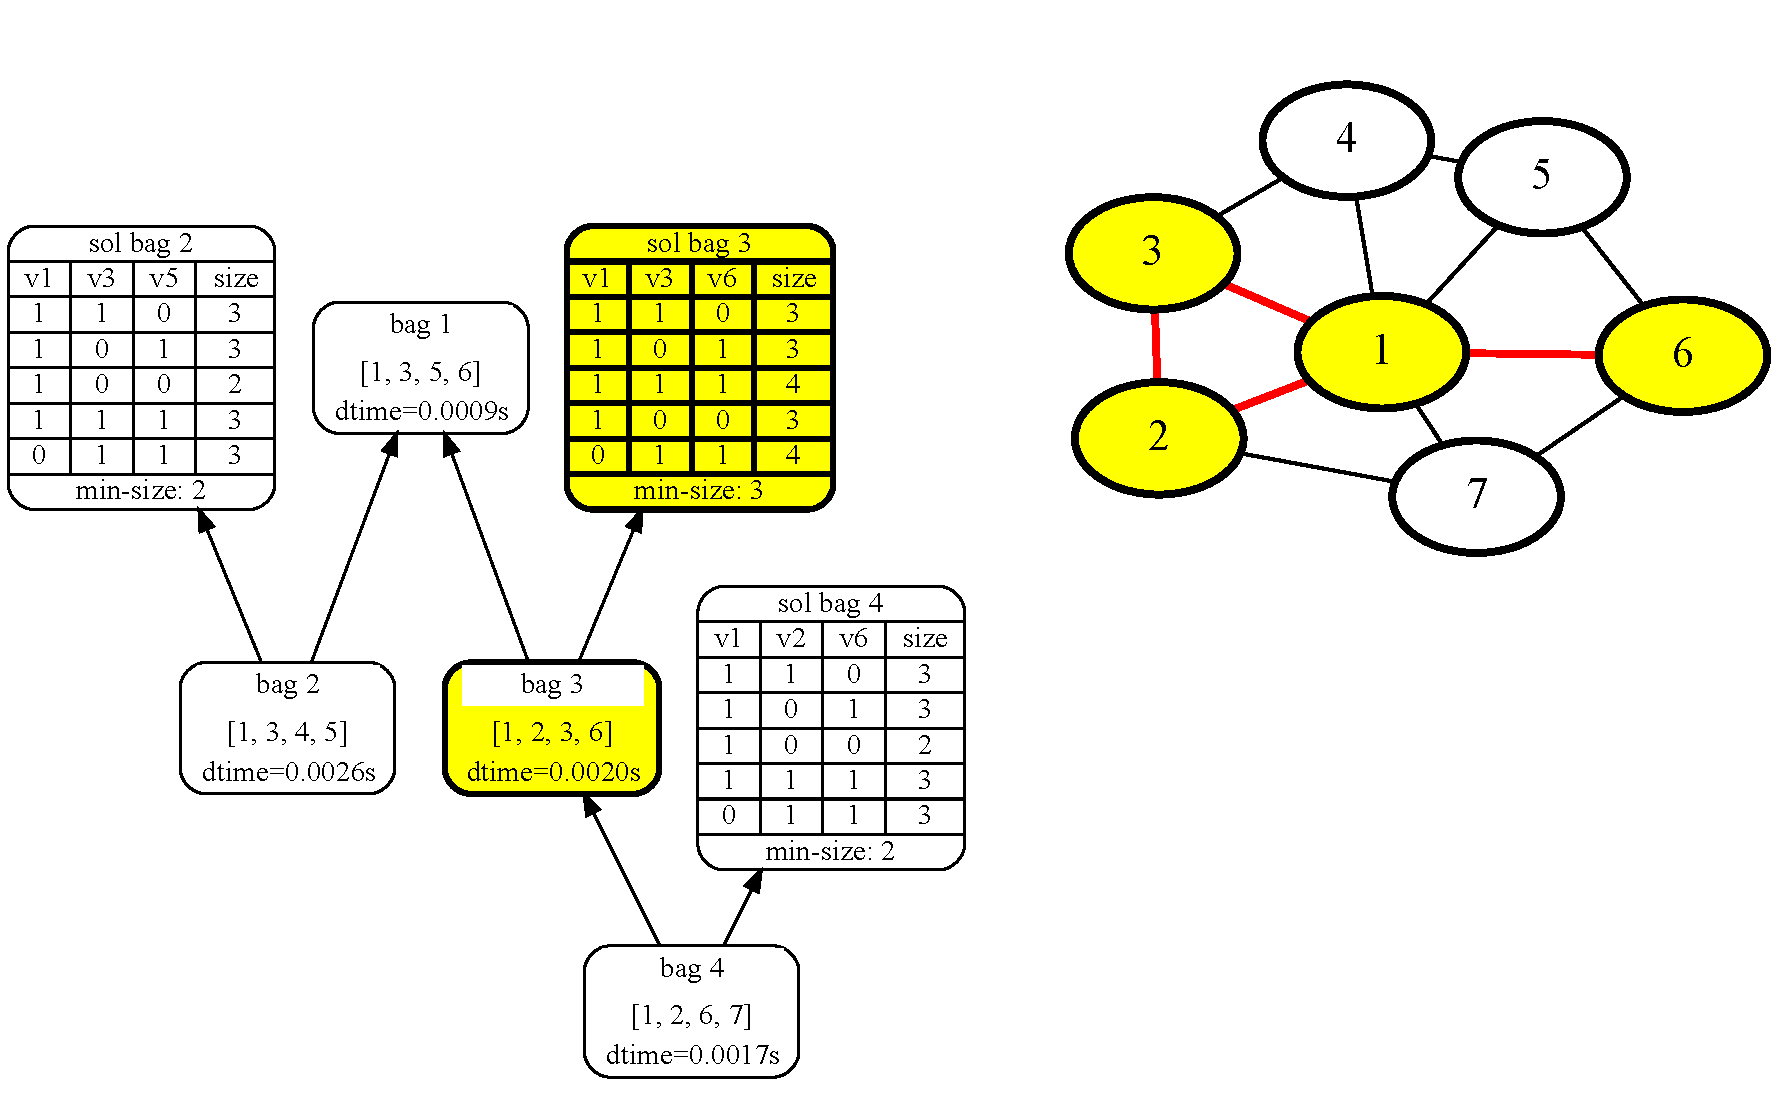
\includegraphics[width=0.9\linewidth,height=0.9\textheight,keepaspectratio]{images/SVGJOIN/default_06sc154.pdf}
	\caption[Joining results from Section \ref{sec:minvc} at step 4/5]{Joining results from Section \ref{sec:minvc} at step 4. Also shifting the second graphic to $40\%$ height of the first image and scaling with scale2 = 1.5 .}
	\label{fig:joinscaled4}
\end{figure}
\begin{figure}[H]
	\centering
	\includegraphics[width=0.9\linewidth,height=0.9\textheight,keepaspectratio]{images/SVGJOIN/default_06sc155.pdf}
	\caption[Joining results from Section \ref{sec:minvc} at step 5]{Joining results from Section \ref{sec:minvc} at step 5. Also shifting the second graphic to $40\%$ height of the first image and scaling with scale2 = 1.5 .}
	\label{fig:joinscaled5}
\end{figure}
%svg_join(['TDStep', 'graph'],
%'Archive/WheelGraph7',
%outname="default_06sc15_rise",
%v_bottom=[1,.85,.7,.55,.4],
%scale2=1.5,
%num_images=5)
\begin{figure}[H]
	\centering
	\includegraphics[width=0.9\linewidth,height=0.9\textheight,keepaspectratio]{images/SVGJOIN/default_06sc15_rise1.pdf}
	\caption[Comprehensive example joining results together step 1/5]{Joining results from Section \ref{sec:minvc} at the first step. Also shifting the second graphic to the bottom edge of the first image and scaling with scale2 = 1.5 .}
	\label{fig:joinscaledrise1}
\end{figure}
\begin{figure}[H]
	\centering
	\includegraphics[width=0.9\linewidth,height=0.9\textheight,keepaspectratio]{images/SVGJOIN/default_06sc15_rise2.pdf}
	\caption[Comprehensive example joining results together step 2/5]{Joining results from Section \ref{sec:minvc} at the second step. Also shifting the second graphic to $15\%$ of the height of the first image and scaling with scale2 = 1.5 .}
	\label{fig:joinscaledrise2}
\end{figure}
\begin{figure}[H]
	\centering
	\includegraphics[width=0.9\linewidth,height=0.9\textheight,keepaspectratio]{images/SVGJOIN/default_06sc15_rise3.pdf}
	\caption[Comprehensive example joining results together step 3/5]{Joining results from Section \ref{sec:minvc} at the third step. Also shifting the second graphic to $30\%$ of the height of the first image and scaling with scale2 = 1.5 .}
	\label{fig:joinscaledrise3}
\end{figure}
\begin{figure}[H]
	\centering
	\includegraphics[width=0.9\linewidth,height=0.9\textheight,keepaspectratio]{images/SVGJOIN/default_06sc15_rise4.pdf}
	\caption[Comprehensive example joining results together step 4/5]{Joining results from Section \ref{sec:minvc} at the fourth step. Also shifting the second graphic to $45\%$ of the height of the first image and scaling with scale2 = 1.5 .}
	\label{fig:joinscaledrise4}
\end{figure}
\begin{figure}[H]
	\centering
	\includegraphics[width=0.9\linewidth,height=0.9\textheight,keepaspectratio]{images/SVGJOIN/default_06sc15_rise5.pdf}
	\caption[Comprehensive example joining results together final image]{Joining results from Section \ref{sec:minvc} at the final step. Also shifting the second graphic to to $60\%$ of the height of the first image and scaling with scale2 = 1.5 .}
	\label{fig:joinscaledrise5}
\end{figure}

%============== Code Snippets ======================================================
\newpage
\section{Code Snippets}

\lstinputlisting[caption={A description of the JSON format used to describe MSO visualization on tree decompositions. See also the formal \textit{TDVisu.schema.json} in \textit{tdvisu}.}, label={lst:jsonapi}]{includes/JsonAPI.txt}

{\lstinputlisting[caption={Tree decomposition in DIMACS format for Figure \ref{fig:tdweelgraph7}},language=json,xleftmargin=5.5cm,xrightmargin=5.8cm,label={lst:wheelgraphtd},numbers=none]{images/WheelGraph7/wheelgraph7.td}}

\begin{lstlisting}[style=custompy, caption={Initializing a Visualization object}, label={lst:visuinit}]
def __init__(self, infile, outfolder) -> None:
	"""Copy needed fields from arguments and create VisualizationData.
	"""
	self.data: VisualizationData = self.inspect_json(infile)
	self.outfolder = outfolder

	self.tree_dec_digraph = None

def inspect_json(self, infile) -> VisualizationData:
	"""Read and preprocess the needed data from the infile into 
	VisualizationData.
	"""
	LOGGER.debug("Reading from: %s", infile)
	visudata = read_json(infile)
	LOGGER.debug("Found keys: %s", visudata.keys())
	
	try:
		_incid = visudata['incidenceGraph']
		_general_graph = visudata['generalGraph']
		_svg_join = visudata.get('svg_join', None)
		
		incid_data: IncidenceGraphData = None
		if _incid:
		_incid['edges'] = [[x['id'], x['list']]
		for x in _incid['edges']]
		incid_data = IncidenceGraphData(**_incid)
		visudata.pop('incidenceGraph')
		general_graph_data: GeneralGraphData = None
		if _general_graph:
		general_graph_data = GeneralGraphData(**_general_graph)
		visudata.pop('generalGraph')
		svg_join_data: SvgJoinData = None
		if _svg_join:
		svg_join_data = SvgJoinData(**_svg_join)
		if 'svg_join' in visudata:
		visudata.pop('svg_join')
		
		self.timeline = visudata['tdTimeline']
		visudata.pop('tdTimeline')
		self.tree_dec = visudata['treeDecJson']
		self.bagpre = self.tree_dec['bagpre']
		self.joinpre = self.tree_dec.get('joinpre', 'Join %d~%d')
		self.solpre = self.tree_dec.get('solpre', 'sol%d')
		self.soljoinpre = self.tree_dec.get('soljoinpre', 'solJoin%d~%d')
		visudata.pop('treeDecJson')
	except KeyError as err:
		raise KeyError(f"Key {err} not found in the input Json.")
	return VisualizationData(incidence_graph=incid_data,
			general_graph=general_graph_data,
			svg_join=svg_join_data,
			**visudata)

\end{lstlisting}\pagebreak

\begin{lstlisting}[style=custompy, caption={SvgJoinData}, label={lst:svgjoindataclass}]
@dataclass
class SvgJoinData:
	"""Class holding different parameters to join the results."""
	base_names: Union[str, Iterable[str]]
	folder: Optional[str] = None
	outname: str = 'combined'
	suffix: str = '%d.svg'
	preserve_aspectratio: str = 'xMinYMin'
	num_images: int = 1
	padding: Union[int, Iterable[int]] = 0
	scale2: Union[float, Iterable[float]] = 1.0
	v_top: Union[None, float, str, 
	Iterable[Union[None, float, str]]] = None
	v_bottom: Union[None, float, str, 
	Iterable[Union[None, float, str]]] = None	
\end{lstlisting}

\begin{lstlisting}[style=custompy, caption={IncidenceGraphData}, label={lst:incidencedata}]
@dataclass
class IncidenceGraphData:
"""Class holding different parameters for the incidence graph."""
	edges: list
	subgraph_name_one: str = 'clauses'
	subgraph_name_two: str = 'variables'
	var_name_one: str = ''
	var_name_two: str = ''
	infer_primal: bool = False
	infer_dual: bool = False
	primal_file: str = 'PrimalGraphStep'
	inc_file: str = 'IncidenceGraphStep'
	dual_file: str = 'DualGraphStep'
	fontsize: int = 16
	penwidth: float = 2.2
	second_shape: str = 'diamond'
	column_distance: float = 0.5
\end{lstlisting}\pagebreak

\begin{lstlisting}[style=custompy, caption={GeneralGraphData}, label={lst:gengraphdata}]
@dataclass
class GeneralGraphData:
	"""Class holding different parameters for the general graph."""
	edges: list
	extra_nodes: Optional[list] = None
	graph_name: str = 'graph'
	file_basename: str = 'graph'
	var_name: str = ''
	sort_nodes: bool = False
	need_adj_nodes: bool = False
	fontsize: int = 20
	first_color: str = 'yellow'
	first_style: str = 'filled'
	second_color: str = 'green'
	second_style: str = 'dotted,filled'
\end{lstlisting}

\begin{lstlisting}[style=custompy, caption={Construct\_dpdb\_visu.py}, label={lst:create-json}]
def create_json(problem: int, tw_file=None, intermed_nodes=False):
	"""Create the JSON for the specified problem instance."""
	with connect() as connection:
		# get type of problem
		with connection.cursor() as cur:
				cur.execute("SELECT name,type,num_bags FROM "
				"public.problem WHERE id=%s", (problem,))
				(name, ptype, num_bags) = cur.fetchone()	
		# select the valid constructor for the problem
		constructor: IDpdbVisuConstruct
		
		if ptype == 'Sat':
			constructor = DpdbSatVisu(
				connection, problem, intermed_nodes)
		elif ptype == 'SharpSat':
			constructor = DpdbSharpSatVisu(
				connection, problem, intermed_nodes)
		elif ptype == 'VertexCover':
			constructor = DpdbMinVcVisu(
				connection, problem, intermed_nodes, tw_file)
		return constructor.construct()
	return {} 
\end{lstlisting}

\begin{lstlisting}[style=custompy, caption={forward\_iterate\_tdg}, label={lst:forward-iterate}]
def forward_iterate_tdg(self, joinpre, solpre, soljoinpre) -> None:
"""Create the final positions of all nodes with solutions."""
	tdg = self.tree_dec_digraph                 # shorten name
	
	for i, node in enumerate(self.timeline):
		if len(node) > 1:
			# solution to be displayed
			id_inv_bags = node[0]
			if isinstance(id_inv_bags, int):
				last_sol = solpre % id_inv_bags
				tdg.node(last_sol, solution_node(
				*(node[1])), shape='record')	
				tdg.edge(self.bagpre % id_inv_bags, last_sol)
			
			else:    # joined node with 2 bags
				suc = self.timeline[i + 1][0]   # get the joined bags
				
				LOGGER.debug('joining %s to %s ', node[0], suc)
				
				id_inv_bags = tuple(id_inv_bags)
				last_sol = soljoinpre % id_inv_bags
				tdg.node(last_sol, solution_node(
				*(node[1])), shape='record')
				
				tdg.edge(joinpre % id_inv_bags, last_sol)
				# edges
				for child in id_inv_bags:  # basically "remove" current
					tdg.edge(
							self.bagpre % child
							if isinstance(child, int) else joinpre % child,
							self.bagpre % suc
							if isinstance(suc, int) else joinpre % suc,
							style='invis',
							constraint='false')
					tdg.edge(self.bagpre % child if isinstance(child, int)
					         else joinpre % child,
					         joinpre % id_inv_bags)
				tdg.edge(joinpre % id_inv_bags, self.bagpre % suc
					if isinstance(suc, int) else joinpre % suc)
\end{lstlisting}

\begin{lstlisting}[style=custompy, caption={backwards\_iterate\_tdg}, label={lst:backward-iterate}]
def backwards_iterate_tdg(self, joinpre, solpre, soljoinpre,
                          view=False) -> None:
	"""Cut the single steps back and update emphasis acordingly."""
	tdg = self.tree_dec_digraph     # shorten name
	last_sol = ""
	
	for i, node in enumerate(reversed(self.timeline)):
		id_inv_bags = node[0]
		LOGGER.debug("%s: Reverse traversing on %s", i, id_inv_bags)
		
		if i > 0:
			# Delete previous emphasis
			prevhead = self.timeline[len(self.timeline) - i][0]
			bag = (self.bagpre % prevhead if isinstance(prevhead,int) 
					else joinpre % tuple(prevhead))
			base_style(tdg, bag)
			if last_sol:
				style_hide_node(tdg, last_sol)
				style_hide_edge(tdg, bag, last_sol)
				last_sol = ""
		
		if len(node) > 1:
			# solution to be displayed
			if isinstance(id_inv_bags, int):
				last_sol = solpre % id_inv_bags
				emphasise_node(tdg, last_sol)
				tdg.edge(self.bagpre % id_inv_bags, last_sol)
			else:  # joined node with 2 bags
				id_inv_bags = tuple(id_inv_bags)
				last_sol = soljoinpre % id_inv_bags
				emphasise_node(tdg, last_sol)
			
		emphasise_node(tdg,
			self.bagpre % id_inv_bags if isinstance(id_inv_bags, int) else 
			joinpre % id_inv_bags)
		_filename = self.outfolder + self.data.td_file + '%d'
		tdg.render(
			view=view, format='svg', filename=_filename %
			(len(self.timeline) - i))

\end{lstlisting}

\begin{lstlisting}[style=custompy, caption={SvgJoinData}, label={lst:svgjoindata}]
@dataclass
class SvgJoinData:
	"""Class for holding different parameters to join the results."""
	base_names: Union[str, Iterable[str]]
	folder: Optional[str] = None
	outname: str = 'combined'
	suffix: str = '%d.svg'
	preserve_aspectratio: str = 'xMinYMin'
	num_images: int = 1
	padding: Union[int, Iterable[int]] = 0
	scale2: Union[float, Iterable[float]] = 1.0
	v_top: Union[None, float, str, 
	             Iterable[Union[None, float, str]]] = 'top'
	v_bottom: Union[None, float, str, 
	                Iterable[Union[None, float, str]]] = None
\end{lstlisting}

%============== Input Examples ======================================================
\section{More Examples}\label{app:input}


\begin{table}[H]
	\centering
	
	\begin{tabular}{|l||c|c|c|c|c|c|c|c|}
		
		\hline
		&$v_{1}$ & $v_{2}$ & $v_{3}$ & $v_{4}$ & $v_{5}$ & $v_{6}$ & $v_{7}$ & $v_{8}$ \\
		\hline 
		1&1 & 1 & 1 & 1 & 1 & 1 & 1 & 1 \\
		2&1 & 1 & 1 & 1 & 1 & 1 & 1 & 0 \\
		3&1 & 1 & 1 & 1 & 0 & 1 & 1 & 1 \\
		4&1 & 1 & 1 & 1 & 0 & 1 & 1 & 0 \\
		5&1 & 1 & 1 & 0 & 1 & 1 & 1 & 0 \\
		6&1 & 1 & 1 & 0 & 1 & 0 & 1 & 0 \\
		7&1 & 1 & 1 & 0 & 0 & 1 & 1 & 0 \\
		8&1 & 1 & 1 & 0 & 0 & 0 & 1 & 0 \\
		9&1 & 1 & 0 & 1 & 1 & 1 & 1 & 0 \\
		10&1 & 1 & 0 & 1 & 0 & 1 & 1 & 0 \\
		11&1 & 1 & 0 & 0 & 1 & 1 & 1 & 0 \\
		12&1 & 1 & 0 & 0 & 1 & 0 & 1 & 0 \\
		13&1 & 1 & 0 & 0 & 0 & 1 & 1 & 0 \\
		14&1 & 1 & 0 & 0 & 0 & 0 & 1 & 0 \\
		15&1 & 0 & 1 & 0 & 0 & 0 & 1 & 0 \\
		16&0 & 1 & 1 & 1 & 0 & 1 & 1 & 1 \\
		17&0 & 1 & 1 & 1 & 0 & 1 & 1 & 0 \\
		18&0 & 1 & 1 & 0 & 0 & 1 & 1 & 0 \\
		19&0 & 1 & 1 & 0 & 0 & 1 & 0 & 0 \\
		20&0 & 1 & 0 & 1 & 0 & 1 & 1 & 0 \\
		21&0 & 1 & 0 & 0 & 0 & 1 & 1 & 0 \\
		22&0 & 1 & 0 & 0 & 0 & 1 & 0 & 0 \\
		\hline
	\end{tabular}
\caption{The satisfying assignments for the formula from Example~\ref{ex:example41}.}
\label{tab:ex41tabx}
\end{table}

\begin{lstlisting}[caption={CNF clauses from example 4.1 in \cite{DiplomarbeitZisser} page 27}, label={lst:clausesDA41},language=json,xleftmargin=5.5cm,xrightmargin=5.8cm]
p cnf 8 10
1 4 6 0
1 -5 0
-1 7 0
2 3 0
2 5 0
2 -6 0
3 -8 0
4 -8 0
-4 6 0
-4 7 0
\end{lstlisting}
\begin{lstlisting}[caption={CNF clauses from random example with 12 units},label={lst:example18-24},language=json,xleftmargin=5.5cm,xrightmargin=5.8cm]
p cnf 18 24
-1 0
-2 0
-3 0
-4 0
-5 0
-6 0
-7 0
-8 0
-9 0
-10 0
-11 0
-12 0
-13 -14 -15 0
-13 -14 16 0
-13 -15 -16 -18 0
-13 -15 -17 0
13 14 16 -17 18 0
13 15 -16 -18 0
-14 -15 16 17 0
-14 15 -17 18 0
-14 15 17 -18 0
-15 -16 -17 18 0
15 -16 -17 -18 0
15 16 17 -18 0
\end{lstlisting}
\lstinputlisting[caption={Edges for example \ref{fig:wheelgraph}}, label={lst:wheelgraph},language=json,xleftmargin=5.5cm,xrightmargin=5.8cm]{images/WheelGraph7/wheelgraph7.tw}
\lstinputlisting[caption={DOT source for visualization of example 4.1}, label={lst:g41digraphdot}]{includes/g41digraphdot}\pagebreak
\lstinputlisting[caption={Small GML output from class \textit{Graphoutput}, Section \ref{sec:chagraphoutput}}, label={lst:g41digraphgml},,language=json,xleftmargin=4.cm,xrightmargin=4cm]{includes/graphml.gml}
\lstinputlisting[caption={Console output by modified \textit{gpusat} with full debugging enabled.}, label={lst:outputgpusat}]{includes/outputGpusatshort.txt}
%==============================================================================
%============== BIBLIOGRAPHY ==================================================
%==============================================================================
\newpage
\listoffigures
\newpage
\listoftables
\renewcommand{\lstlistlistingname}{Listings}
\lstlistoflistings
\newpage
\printbibliography
%\bibliography{bibtex}{}
%\bibliographystyle{ieeetr}
\end{document}
